%

%Note: LaTeX Beamer taken from the website: https://www.sharelatex.com/templates/presentations/conference-presentation
%Note: to find out the RGB code for dolphin: https://tex.stackexchange.com/questions/66465/how-to-get-actual-values-of-colour-theme-colours-in-beamer
%Note: to convert eps files to pdf: https://docupub.com/pdfconvert/

\documentclass[xcolor=table]{beamer}
\usepackage{appendixnumberbeamer}

\usepackage{subcaption}

% Change the margin
%\setbeamersize{text margin left = 2pt, text margin right = 2pt}

\setbeamertemplate{footline}[frame number]
\setbeamertemplate{headline}{}
% There are many different themes available for Beamer. A comprehensive
% list with examples is given here:
% http://deic.uab.es/~iblanes/beamer_gallery/index_by_theme.html
% You can uncomment the themes below if you would like to use a different
% one:
%\usetheme{AnnArbor}
%\usetheme{Antibes}
%\usetheme{Bergen}
%\usetheme{Berkeley}
%\usetheme{Berlin}
%\usetheme{Boadilla}
%\usetheme{boxes}
%\usetheme{CambridgeUS}
%\usetheme{Copenhagen}
%\usetheme{Darmstadt}
\usetheme{default}
%\usetheme{Frankfurt}
%\usetheme{Goettingen}
%\usetheme{Hannover}
%\usetheme{Ilmenau}
%\usetheme{JuanLesPins}
%\usetheme{Luebeck}
%\usetheme{Madrid}
%\usetheme{Malmoe}
%\usetheme{Marburg}
%\usetheme{Montpellier}
%\usetheme{PaloAlto}
%\usetheme{Pittsburgh}
%\usetheme{Rochester}
%\usetheme{Singapore}
%\usetheme{Szeged}
%\usetheme{Warsaw}
\makeatletter
\definecolor{beamer@blendedblue}{RGB}{164, 92, 92} % changed this

%\setbeamercolor{normal text}{fg=black,bg=white}
%\setbeamercolor{alerted text}{fg=red}
%\setbeamercolor{example text}{fg=green!50!black}

\setbeamercolor{structure}{fg=beamer@blendedblue}
%\useinnertheme{rounded}

%\renewcommand{\labelitemi}{$\bullet$}
%\renewcommand{\labelitemii}{$\cdot$}
%\renewcommand{\labelitemiii}{$\diamond$}
%\renewcommand{\labelitemiv}{$\ast$}

%colors
\usecolortheme{dolphin}
\usepackage{color}
\definecolor{mycolor1}{RGB}{184, 184, 184}
\definecolor{mycolor2}{RGB}{252, 196, 108}
\definecolor{mycolor3}{RGB}{164, 92, 92}
\definecolor{mycolor4}{RGB}{76, 60, 52}
\definecolor{mycolor5}{RGB}{164, 248, 208}
\definecolor{mycolor6}{RGB}{116, 112, 112}
\definecolor{mycolor7}{RGB}{116, 116, 52}

\usepackage{fnpct}

\usepackage{subcaption}

\usepackage{newpxtext}


%fonts
\usefonttheme{professionalfonts}

%Other packages
\usepackage{bm}
\setbeamercovered{transparent}
\usepackage[section]{placeins}
\usepackage{epstopdf}
\usepackage[table]{xcolor}
\usepackage{graphicx} %Useful to resize large tables into the frame using \resizebox 
\usepackage{grffile} %Documentation: http://ctan.sharelatex.com/tex-archive/macros/latex/contrib/oberdiek/grffile.pdf
\usepackage{marvosym}
\usepackage[style=british]{csquotes}
\def\signed #1{{\leavevmode\unskip\nobreak\hfil\penalty50\hskip2em
		\hbox{}\nobreak\hfill #1
		\parfillskip=0pt \finalhyphendemerits=0 \endgraf}}

\newsavebox\mybox
\newenvironment{aquote}[1]
{\savebox\mybox{#1}\begin{quote}}
	{\vspace*{1mm}\signed{\usebox\mybox}\end{quote}}

\usepackage{verse}
\newcommand{\attrib}[1]{
	\nopagebreak{\raggedleft\footnotesize #1\par}}

%for checkmarks
\usepackage{tikz}

%For equations
\usepackage{amsmath, amssymb}
\usepackage{bbm}

	%Tables
	\usepackage{tabularx}
	\usepackage{multirow}
	\usepackage{multicol} 
	\usepackage{booktabs}%\usepackage{booktabs, calc} %This is the package to use to have nice-looking tables. More documentation on the tables in LateX: https://www.tug.org/pracjourn/2007-1/mori/mori.pdf
	\usepackage{threeparttable}  
	\usepackage[table]{xcolor}
	\usepackage{colortbl}
	\usepackage{lmodern}
	\usepackage{booktabs}
	\usepackage{pgfplots}

% Count slides
\setcounter{MaxMatrixCols}{10}

\graphicspath{{../figuras/}}
%\graphicspath{{../tablas/}}

% Commands -
\newcommand{\extractRGB}[1]{\extractcolorspecs{#1}{\model}{\dolphin} \convertcolorspec{\model}{\dolphin}{RGB}\printcol \printcol}
\setbeamertemplate{caption}{\raggedright\insertcaption\par} %to prevent beamer from putting "figure" in front of a caption
\setbeamertemplate{navigation symbols}{}

%Code to create sections with title pages in Beamer slides
\AtBeginSection[]{
	\begin{frame}[plain]
		\vfill
		\centering
		\begin{beamercolorbox}[sep=8pt,center,shadow=true,rounded=true]{title}
			\usebeamerfont{title}\insertsectionhead\par%
		\end{beamercolorbox}
		\vfill
	\end{frame}
}

\title{Sala Situacional COVID-19, Región Cusco\footnote{Análisis con información de la región hasta el 11 de Junio del 2022}}
\author{Fátima Concha \& Joel Sumerente} 
\institute{Dirección de Epidemiología e Investigación \\ \textbf{\color{mycolor3}DEIS, GERESA - Cusco}}
\date{Semana Epidemiológica 23, 2022}

\begin{document}
	%------------------------------------------------------------------------------------------------------------------------------------------------------------------------------------------------------------------------------------------
	% TITLE PAGE 
	%------------------------------------------------------------------------------------------------------------------------------------------------------------------------------------------------------------------------------------------
	\setbeamercovered{invisible}
	\begin{frame}[plain]
		\titlepage
	\end{frame}

	%------------------------------------------------------------------------------------------------------------------------------------------------------------------------------------------------------------------------------------------
	% INTRODUCTION 
	%------------------------------------------------------------------------------------------------------------------------------------------------------------------------------------------------------------------------------------------
	
	\setcounter{subsection}{1}
	\begin{frame}[label=indice]
		\frametitle{Índice}
		\vspace{-.5cm}
		\begin{itemize}
			\item Indicadores epidemiológicos.
			\begin{itemize}
				\item Nacional: Variantes, cobertura vacuna, mortalidad, RT, ocupación de camas UCI y no UCI a nivel regional. \hyperlink{epi_nacional}{\beamergotobutton{epi. nacional.}}
				\item Regional: Curva epidémica, incidencia, tasa de positividad, variantes ( \hyperlink{variantes}{\beamergotobutton{variantes}}), defunciones, RT por distrito, exceso de defunciones, letalidad, mortalidad, y mortalidad por grupos de edad e hitos de vacunación.  \hyperlink{epi_cusco}{\beamergotobutton{epi. cusco.}} 
			\end{itemize} 
			\item Cobertura de Vacunación ( \hyperlink{cobertura_vacuna}{\beamergotobutton{cobertura}}). 
			\item Indicadores de gestión hospitalaria.
			\begin{itemize}
				\item Ocupación camas UCI y no UCI a nivel regional y por hospital. \hyperlink{camas}{\beamergotobutton{camas hosp.}} 
			\end{itemize}
			\item Indicadores por provincias.
			\begin{itemize}
				\item Incidencia, tasa de mortalidad, tasa de letalidad, tasa de positividad PCR, AG, y exceso de mortalidad. \hyperlink{provincias}{\beamergotobutton{provincias}}
			\end{itemize}
			\item Resumen y recomendaciones. \hyperlink{resumen}{\beamergotobutton{resumen}} \hyperlink{recomendaciones}{\beamergotobutton{recomendaciones}}
			\item Links útiles. \hyperlink{links}{\beamergotobutton{links}} \hfill \hyperlink{vacunas_60}{\beamergotobutton{apendice}}
		\end{itemize}
	\end{frame}
	
	%------------------------------------------------------------------------------------------------------------------------------------------------------------------------------------------------------------------------------------------
	% SECCIÓN 1: Indicadores Epidemiológicos, Nivel Nacional
	%------------------------------------------------------------------------------------------------------------------------------------------------------------------------------------------------------------------------------------------
	\section{Indicadores Epidemiológicos, Nivel Nacional}
%	
%	\begin{frame}[label=epi_nacional]
%	\frametitle{Tendencia de Variantes en Lima y la Sierra Selva Sur}
%	\vspace{-.5cm}
%	\begin{figure}
%		\centering
%		\begin{subfigure}[b]{0.40\textwidth}
%			\centering
%			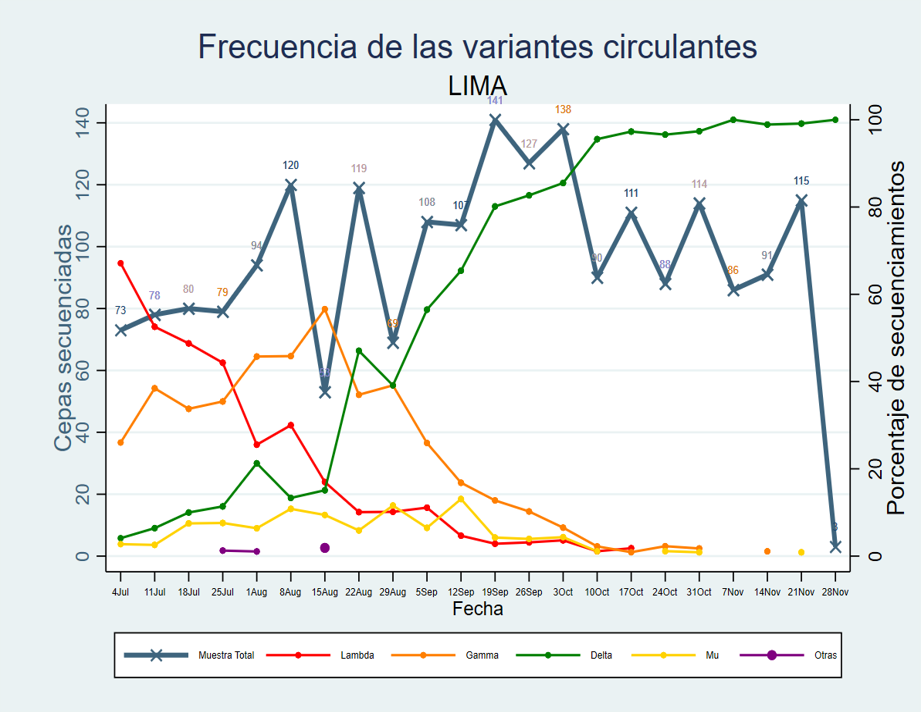
\includegraphics[width=\textwidth]{../sala_nacional/variantes_lima.png}
%			\caption{Lima}
%			%\label{fig:}
%		\end{subfigure}
%		\hfill
%		\begin{subfigure}[b]{0.42\textwidth}
%			\centering
%			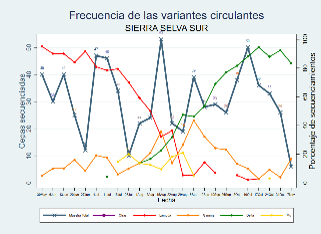
\includegraphics[width=\textwidth]{../sala_nacional/variantes_sierra_sur.png}
%			\caption{Sierra Selva Sur}
%			%\label{fig:70 a 79 años}
%		\end{subfigure}
%	\end{figure}
%	{\tiny Fuente: Lescano, Orellana, Fano, Pino, y Flores. Situación Epidemiológica de la COVID-19 al 26 de Febrero del 2022.\\} 
%	\vspace{0.01cm}
%	$\rightarrow$ 100\% ómicron en Lima y Callao en la SE05, 33 y 8 muestras respectivamente.\\
%	$\rightarrow$ Omicrón detectada en Lima: 3/90 muestras.\\
%	$\rightarrow$ Resultados de 2-3 semanas atrás. Vacíos en 10 regiones.\\	
%\end{frame}
%
%\begin{frame}[label=epi_nacional]
%	\frametitle{Casos nacionales bajan 36.7\%, cuarta caída fuerte?}
%	\vspace{.1cm}
%	\begin{figure}
%		\centering
%		\begin{subfigure}[b]{0.35\textwidth}
%			\centering
%			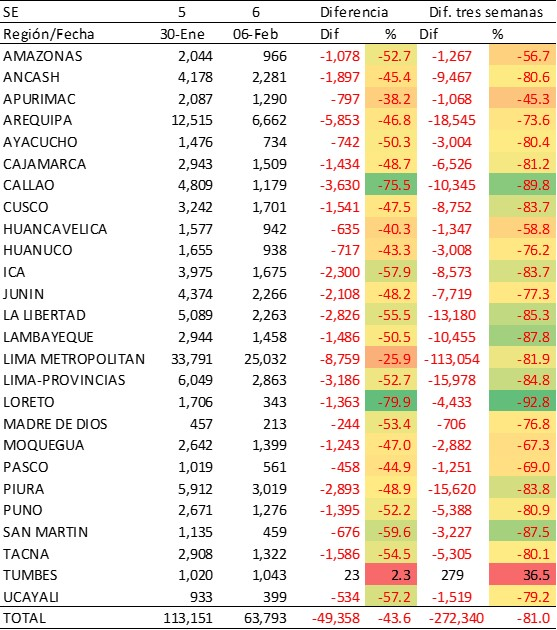
\includegraphics[width=\textwidth]{../sala_nacional/Casos_Nacionales_3ra_ola.jpg}
%			%\label{fig:}
%		\end{subfigure}
%		\begin{tikzpicture}[overlay]
%		\draw[mycolor2, thick] (-2.05,2.73) circle [x radius=2.5cm, y radius=.15cm, rotate=0];
%		\end{tikzpicture}
%		\hfill
%		\begin{subfigure}[b]{0.55\textwidth}
%			\centering
%			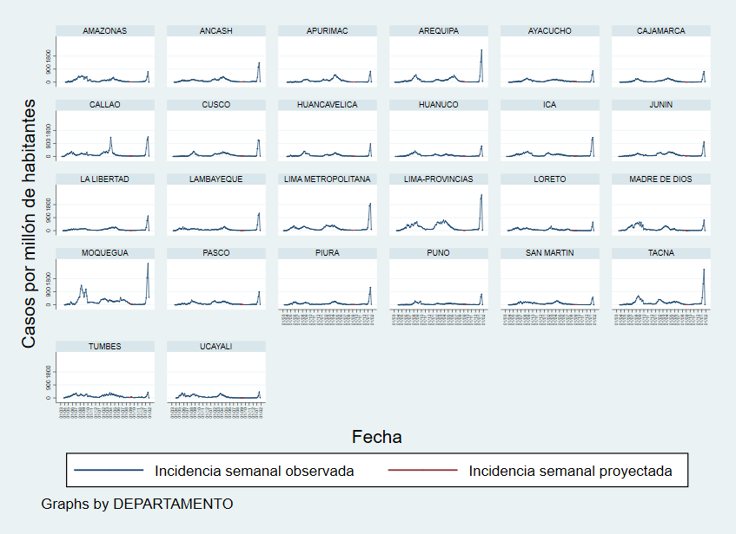
\includegraphics[width=\textwidth]{../sala_nacional/Casos_Nacionales_3ra_ola_02.jpg}
%			%\label{fig:70 a 79 años}
%		\end{subfigure}
%		\begin{tikzpicture}[overlay]
%		\draw[mycolor2, ultra thick] (-4.30,3.20) circle [x radius=.47cm, y radius=.47cm, rotate=0];
%		\end{tikzpicture}
%	\end{figure}
%	{\tiny Fuente: Lescano, Orellana, Fano, Pino, y Flores. Situación Epidemiológica de la COVID-19 al 19 de Febrero del 2022.\\} 
%	\vspace{0.01cm}
%	$\rightarrow$ Sólo sube Tumbes, 139\%, crece nueve semanas.\\
%	$\rightarrow$ La costa norte y Centro caen menos fuertemente.\\
%	$\rightarrow$ Todas las regiones menos Tumbes crecen >22\%.\\
%	$\rightarrow$ Casos caen masiva, simultanea y proporcionalmente en multiples regiones.\\
%\end{frame}
%
%\begin{frame}[label=epi_nacional]
%	\frametitle{Positividad antigénica cae 7.20\%, cuarta y fuerte baja}
%	\vspace{-.1cm}
%	\begin{figure}
%		\centering
%		\begin{subfigure}[b]{0.35\textwidth}
%			\centering
%			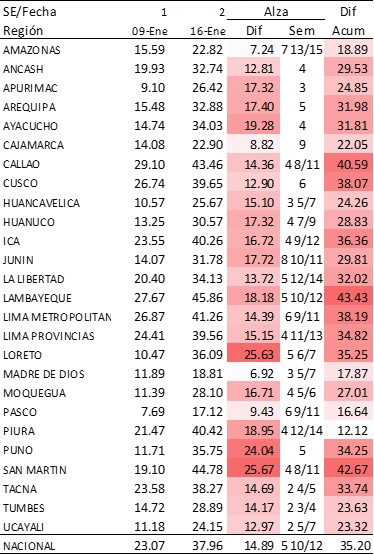
\includegraphics[width=\textwidth]{../sala_nacional/Positividad_Antigenica_3ra_ola.jpg}
%			%\label{fig:}
%		\end{subfigure}
%		\begin{tikzpicture}[overlay]
%			\draw[mycolor2, thick] (-2.10,4.45) circle [x radius=2.4cm, y radius=.15cm, rotate=0];
%		\end{tikzpicture}
%		\hfill
%		\begin{subfigure}[b]{0.60\textwidth}
%			\centering
%			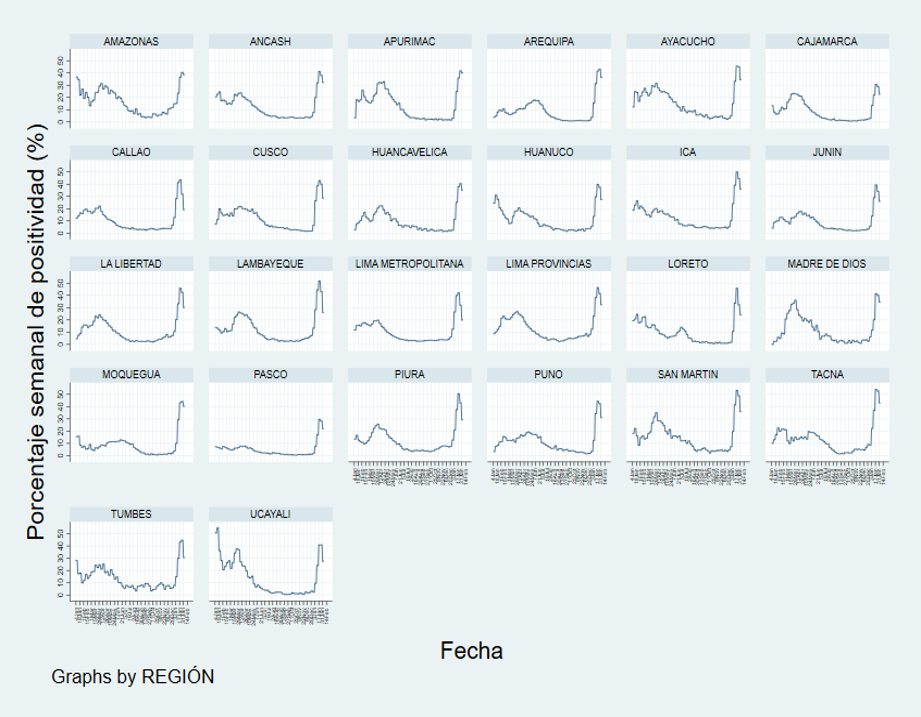
\includegraphics[width=\textwidth]{../sala_nacional/Porcentaje_Positivos_3ra_ola_regiones.jpg.png}
%			%\label{fig:70 a 79 años}
%		\end{subfigure}
%		\begin{tikzpicture}[overlay]
%			\draw[mycolor2, ultra thick] (-4.70,3.60) circle [x radius=.50cm, y radius=.50cm, rotate=0];
%		\end{tikzpicture}
%	\end{figure}
%	{\tiny Fuente: Lescano, Orellana, Fano, Pino, y Flores. Situación Epidemiológica de la COVID-19 al 19 de Febrero del 2022.\\} 
%	\vspace{0.01cm}
%		$\rightarrow$ Todas las regiones bajan por al menos tres semanas.\\
%\end{frame}

\begin{frame}
	\frametitle{Vacunación COVID 19 en el Perú}
	\vspace{-.5cm}
	\begin{center}
		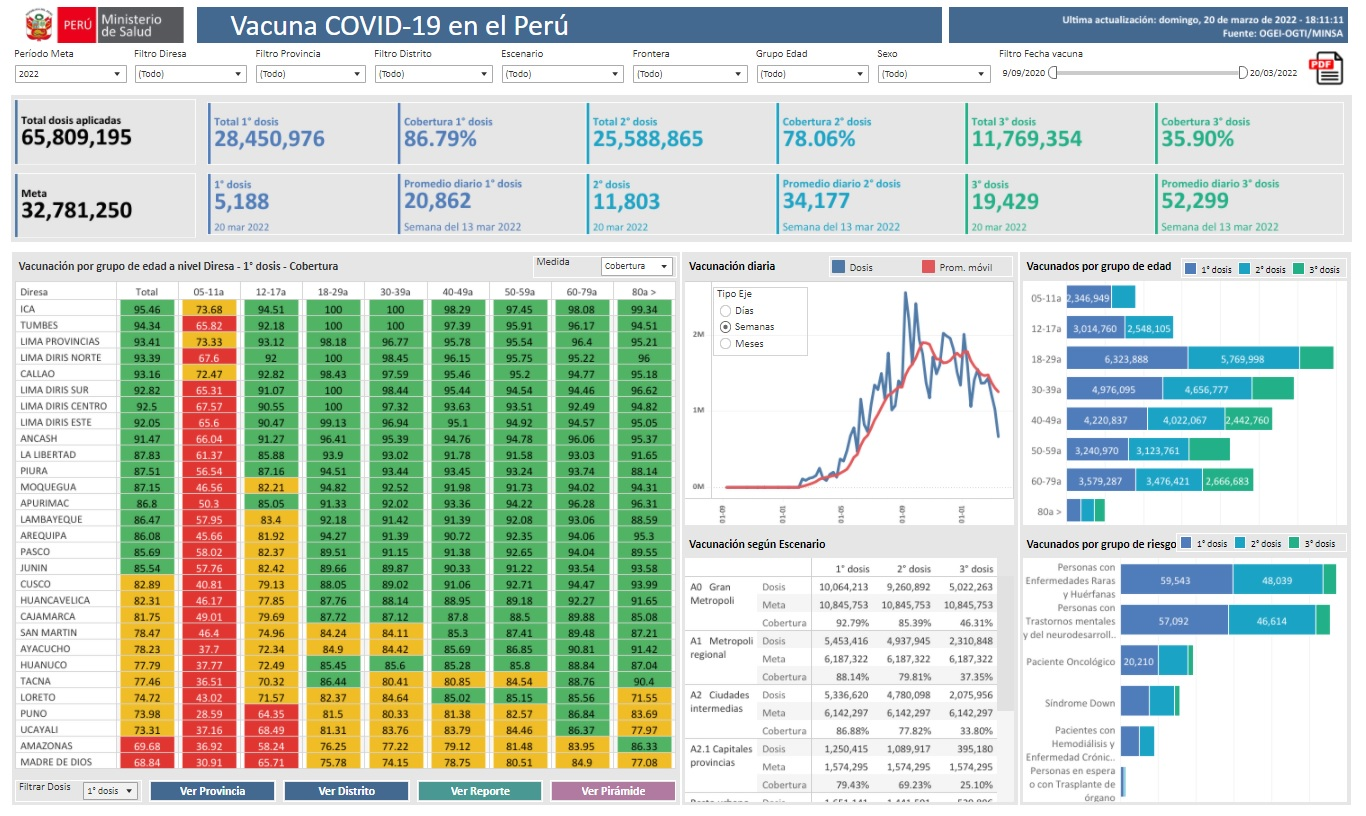
\includegraphics[width=1\linewidth]{../sala_nacional/vacunas_nacional.jpeg} 
	\end{center}

%	\begin{tikzpicture}[overlay]
%		\draw[mycolor5, very thick] (9.5,3.40) circle [x radius=3.0cm, y radius=.58cm, rotate=90];
%	\end{tikzpicture}
	{\tiny Fuente:REUNIS (Repositorio Único Nacional de Información en Salud). Consultado el 11 de Junio del 2022.\\} 
	\vspace{0.01cm}
%	$\searrow$ Cusco pasa al puesto 15.
\end{frame}

\begin{frame}
		\frametitle{Mortalidad por Regiones}
		\vspace{-.2cm}
		\begin{center}
			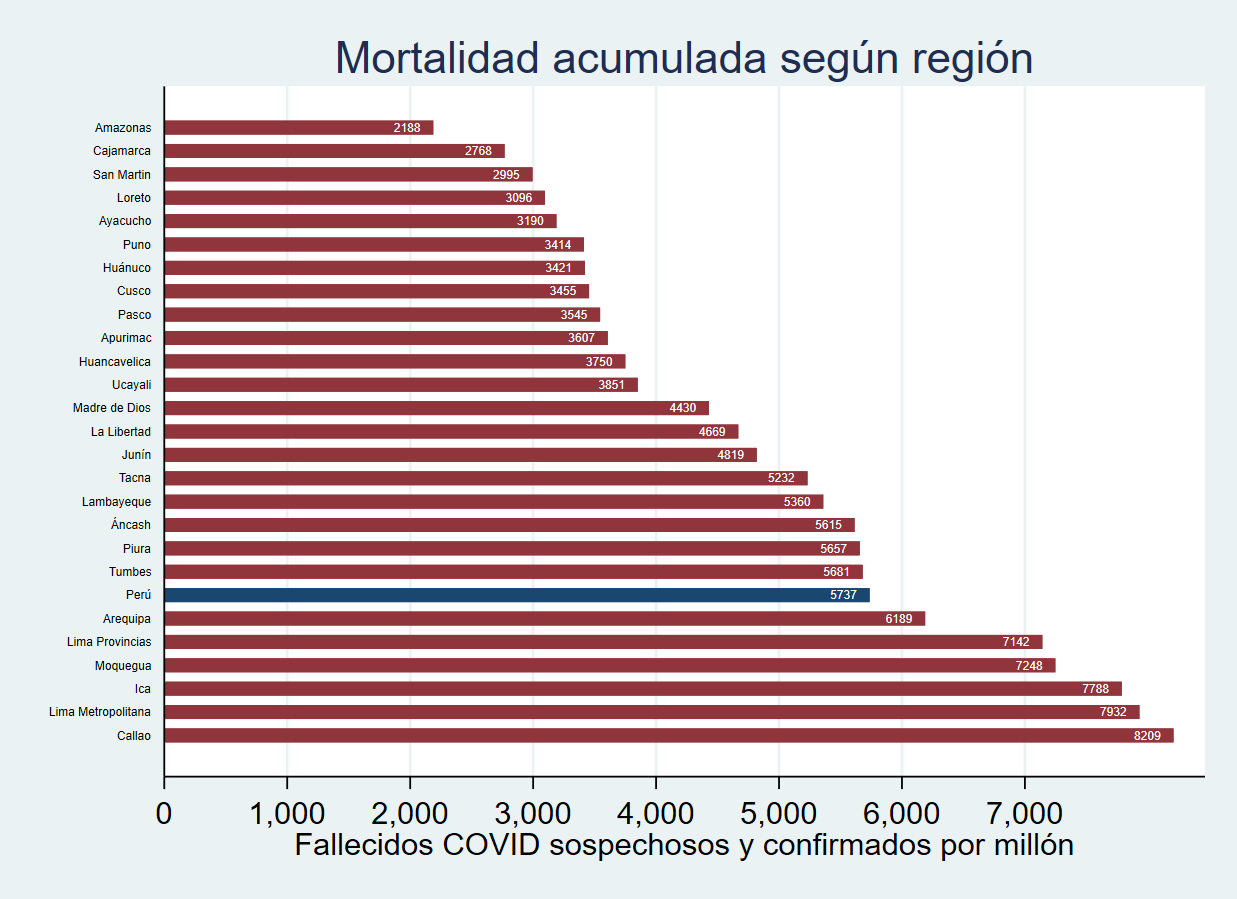
\includegraphics[width=0.75\linewidth]{../sala_nacional/mortalidad_regional.png}
		\end{center}
		\begin{tikzpicture}[overlay]
		\draw[mycolor2, thick] (3.5,4.55) circle [x radius=2.cm, y radius=.13cm, rotate=0];
		\end{tikzpicture}
		{\tiny Fuente: Lescano, Orellana, Fano, Pino, y Flores. Situación Epidemiológica de la COVID-19 al 11 de Junio del 2022.\\}
\vspace{0.01cm}
$\nearrow$ Cusco se mantiene en el puesto 8, con $ 3,450 $ defunciones por COVID-19 por millón de habitantes. \\
\end{frame}

\begin{frame}
	\frametitle{Defunciones Semanales por Regiones}
\vspace{-.2cm}
\begin{center}
	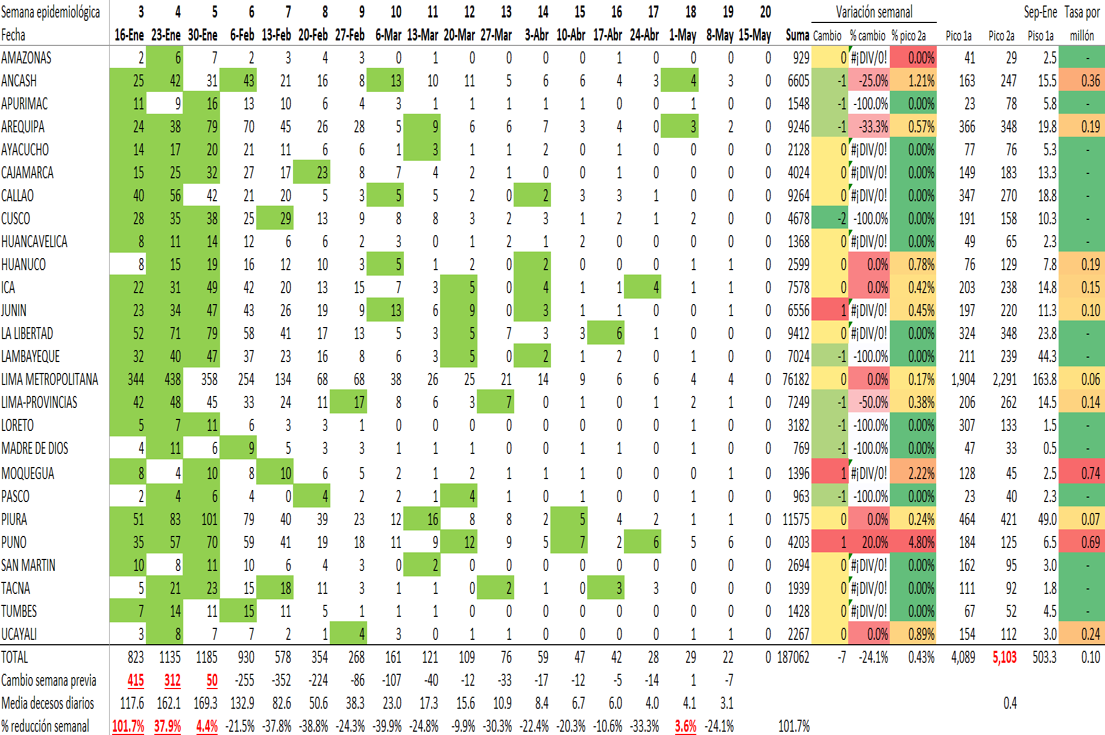
\includegraphics[width=0.55\linewidth]{../sala_nacional/defunciones_regional.png}
\end{center}
\begin{tikzpicture}[overlay]
	\draw[mycolor2, ultra thick] (5.2,3.35) circle [x radius=3.8cm, y radius=.1cm, rotate=0];
\end{tikzpicture}
{\tiny Fuente: Lescano, Orellana, Fano, Pino, y Flores. Situación Epidemiológica de la COVID-19 al 11 de Junio del 2022.\\
%Nota 1: Sube Piura. \\
%Nota 2: Mayor valor en 21 semanas.\\	
\textbf{Riesgos}:\\
			Más fallecidos en seis semanas.\\
			Lima metropolitana incrementa 8 fallecidos, crece dos semanas.\\
			DIRIS Lima Centro y Este suben 3-5 fallecidos.\\
			Costa centro incrementa en 53.3\%.\\
			>25 años aumentan >4 fallecidos, menos el grupo de 70-79 años.\\
\textbf{Menor Riesgo}: \\
			Todas las macro-regiones menos Costa centro disminuyen o se estancan.\\	
			}
\vspace{0.01cm}
$\rightarrow$ {\color{mycolor5}Cusco}: Las defunciones representan un $0.63\% $ del pico de la segunda ola.\\
\end{frame}
	
	\begin{frame}
		\frametitle{Número Reproductivo Efectivo por Regiones}
		\vspace{-.5cm}
		\begin{center}
			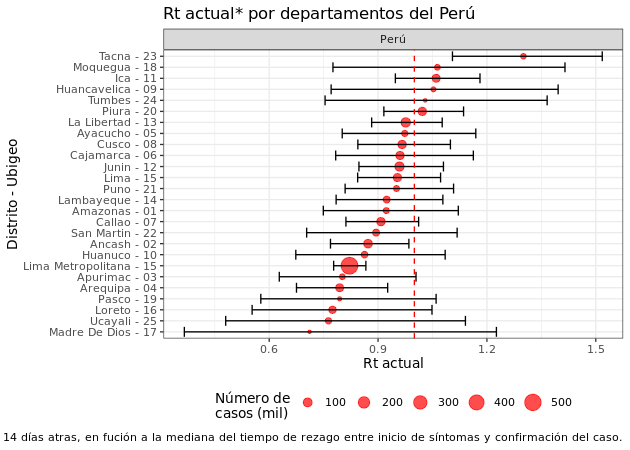
\includegraphics[width=0.71\linewidth]{../sala_nacional/rt_regional.png}
		\end{center}
		\begin{tikzpicture}[overlay]
		\draw[mycolor2, ultra thick] (5.35,3.87) circle [x radius=3.4cm, y radius=.18cm, rotate=0];
		\end{tikzpicture}
	{\tiny Fuente: CDC MINSA. Reporte de Vigilancia COVID-19, Perú 2022. Actualización: 2022-06-11.\\}
	\vspace{0.01cm}
	$\rightarrow$ El número reproductivo efectivo (RT) indica la dinámica de la enfermedad; si es menor a $ 1 $, existe control de la epidemia. \\
	$\nearrow$ Cusco se encuentra a la posición 12 con un RT de $0.80$ $ [0.75-0.85]$.

	\end{frame}

  \begin{frame}
	\frametitle{Ocupación de Camas UCI Comparativo por Regiones}
	\vspace{-.2cm}
	\begin{center}
		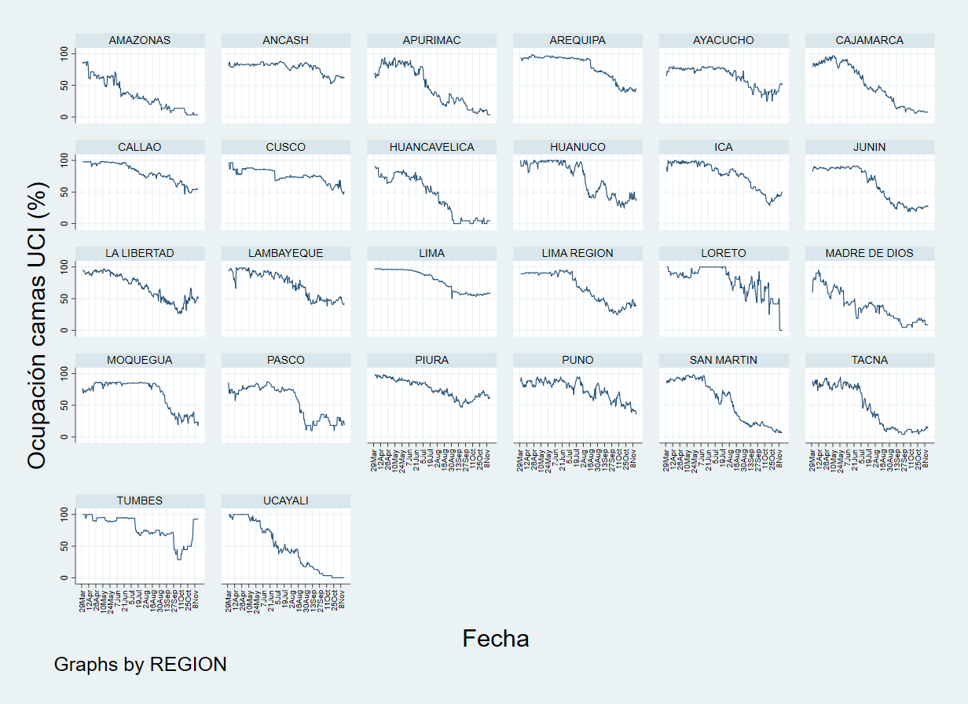
\includegraphics[width=0.60\linewidth]{../sala_nacional/camas_regional.png}
	\end{center}
	\begin{tikzpicture}[overlay]
	\draw[mycolor2, ultra thick] (4.08,3.75) circle [x radius=.50cm, y radius=.50cm, rotate=0];
	\end{tikzpicture}
	{\tiny Fuente: Lescano, Orellana, Fano, Pino, y Flores. Situación Epidemiológica de la COVID-19 al 11 de Junio del 2022. \\
	\textbf Perú: 990 camas libres, baja 5.1\% -  Lima: 380 camas libres, bajo 3.1\%. \\
	\textbf Suben*: \\
	Costa: Tumbes, Piura, Lambayeque, Ancash, Callao y Arequipa.\\
	Otros: San Martin.\\
	\textbf Cuatro regiones suben>1 semana: \\
	Ancash sube 13.1\% en 2 sem.\\
	Arequipa sube 6.7\% en 2 sem.\\
	Piura sube 2.1\% en 2 sem.\\
	Tumbes sube 16.7\% sube en 2 sem.\\
	\textbf >Que media: \\
	La Libertad (52.0\%), Tumbes (50.0\%), Ancash (49.0\%), Arequipa (23.8\%), Piura (21.6\%), Lima metropolitana (11.9\%), Moquegua (11.8\%) y Callao (11.7\%).
	Cinco de estas ocho regiones suben esta semana.\\
	El número de camas UCI ocupadas esta semana sube en Ancash y Callao, y no baja en Piura.\\
} 
	\vspace{0.01cm}
%	$\nearrow$ Solo tres de estas 13 regiones suben.
	
\end{frame}
	\begin{frame}
	\frametitle{Ocupación de Camas UCI por Regiones}
	\vspace{-.5cm}
	\begin{center}
		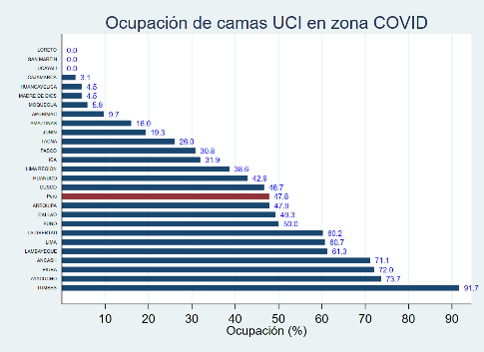
\includegraphics[width=0.75\linewidth]{../sala_nacional/uci_regional.png}
	\end{center}
	\begin{tikzpicture}[overlay]
	\draw[mycolor2, thick] (5.6,3.18) circle [x radius=3.9cm, y radius=.15cm, rotate=0];
\end{tikzpicture}
	{\tiny Fuente: Lescano, Orellana, Fano, Pino, y Flores. Situación Epidemiológica de la COVID-19 al 11 de Junio del 2022.\\}
	\vspace{0.1cm}
	$\searrow$ Cusco se mantiene en la posición 17.
\end{frame}
	
	\begin{frame}
		\frametitle{Ocupación de Camas No UCI por Regiones}
		\vspace{-.5cm}
		\begin{center}
			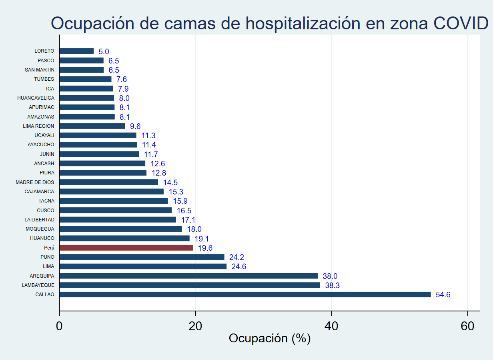
\includegraphics[width=0.75\linewidth]{../sala_nacional/nouci_regional.png} 
		\end{center}
		\begin{tikzpicture}[overlay]
		\draw[mycolor2, thick] (3.8,3.35) circle [x radius=2.8cm, y radius=.15cm, rotate=0];
		\end{tikzpicture}
		{\tiny Fuente: Lescano, Orellana, Fano, Pino, y Flores. Situación Epidemiológica de la COVID-19 al 11 de Junio del 2022. \\} 
		\vspace{0.01cm}
		$\nearrow$ Cusco baja a la posición 16.	
		\hyperlink{indice}{\beamergotobutton{Índice}} 
	\end{frame}


	%------------------------------------------------------------------------------------------------------------------------------------------------------------------------------------------------------------------------------------------
% SECCIÓN 2: Indicadores Epidemiológicos, Región Cusco
%------------------------------------------------------------------------------------------------------------------------------------------------------------------------------------------------------------------------------------------
\section{Indicadores Epidemiológicos, Región Cusco}
	\begin{frame}
		\frametitle{Curva de Sintomáticos y Asintomáticos Semanales}
		\vspace{-.5cm}
		\begin{center}
			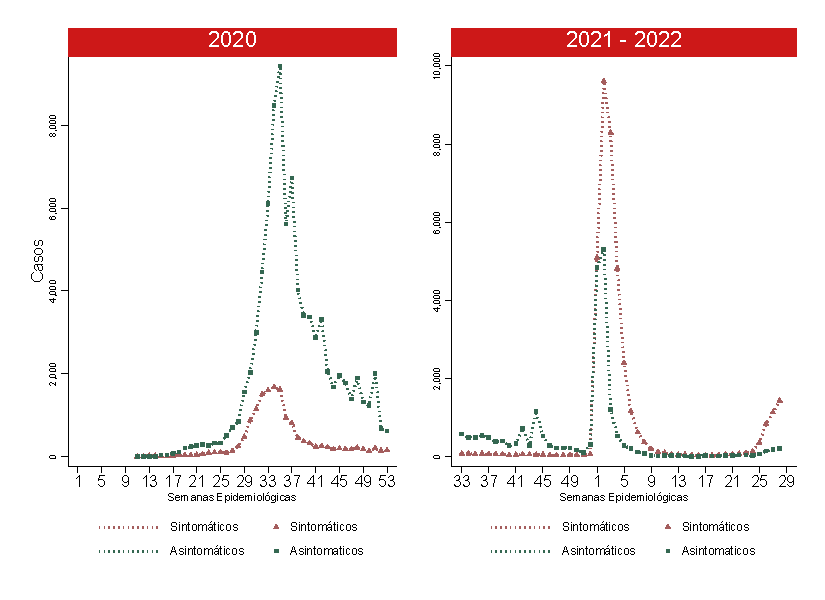
\includegraphics[width=0.9\linewidth]{../figuras/sintomaticos_20_21_22.pdf}
		\end{center} 
		{\tiny Fuente de datos: SISCOVID, NOTICOVID.}
	\end{frame}
	
	\begin{frame}[label=epi_cusco]
		\frametitle{Curva del Total de Casos Positivos Semanales}
		\vspace{-.5cm}
		\begin{center}
			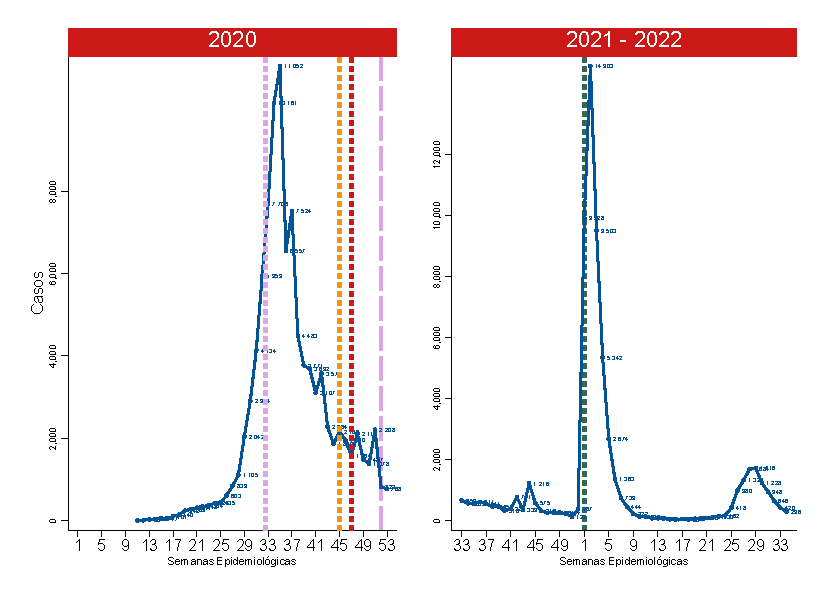
\includegraphics[width=.9\linewidth]{../figuras/positivos_semanales_20_21_22.pdf}
		\end{center}
		{\tiny Fuente de datos: SISCOVID, NOTICOVID.} \\
%			Nota: {\color{mycolor1} --- ---: Navidad}, {\color{mycolor1} - -: Año Nuevo}, {\color{mycolor2} - -: Semana Santa}, {\color{mycolor3} - -: Elecciones Primera Vuelta}, {\color{mycolor4} $- \cdot$: Elecciones Segunda Vuelta}. \\}	
	\end{frame}
	
	\begin{frame}[label=TipoPrueba]
		\frametitle{Curva Epidémica de Sintomáticos por Tipo de Prueba}
		\vspace{-.15cm}
		\begin{center}
			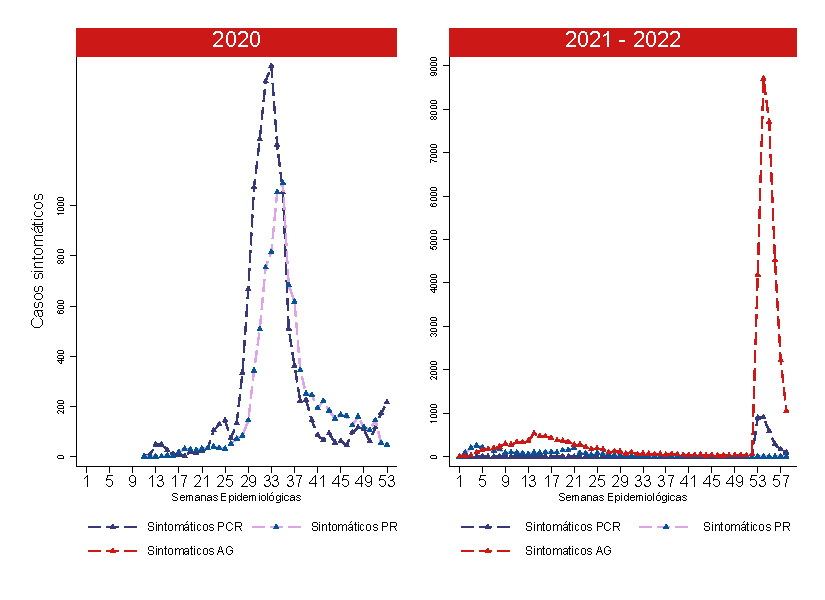
\includegraphics[width=0.7\linewidth, trim={0cm 0cm 0cm 0cm},clip]{../figuras/sinto_prueba_20_21_22.pdf}
		\end{center}
	\vspace{-.5cm}
		{\tiny Fuente de datos: SISCOVID, NOTICOVID.}\\
		Ver detalles de sintomáticos por tipo de prueba para cada provincia haciendo click en los siguientes enlaces:
		\hyperlink{Acomayo}{\beamergotobutton{Acomayo}} 
		\hyperlink{Anta}{\beamergotobutton{Anta}} 
		\hyperlink{Calca}{\beamergotobutton{Calca}} 
		\hyperlink{Canas}{\beamergotobutton{Canas}} \hyperlink{Chumbivilcas}{\beamergotobutton{Chumbivilcas}}
		\hyperlink{Canchis}{\beamergotobutton{Canchis}} 
		\hyperlink{Cusco}{\beamergotobutton{Cusco}}
		\hyperlink{Espinar}{\beamergotobutton{Espinar}}
		\hyperlink{laconvecion}{\beamergotobutton{La Convencion}}
		\hyperlink{Paruro}{\beamergotobutton{Paruro}} \hyperlink{Paucartambo}{\beamergotobutton{Paucartambo}}
		\hyperlink{Quispicanchi}{\beamergotobutton{Quispicanchi}}
		\hyperlink{Urubamba}{\beamergotobutton{Urubamba}}
		\end{frame}
	
	\begin{frame}
		\frametitle{Tasa de Crecimiento del Total de Casos por Semana}
		\vspace{-.5cm}
		\begin{center}
			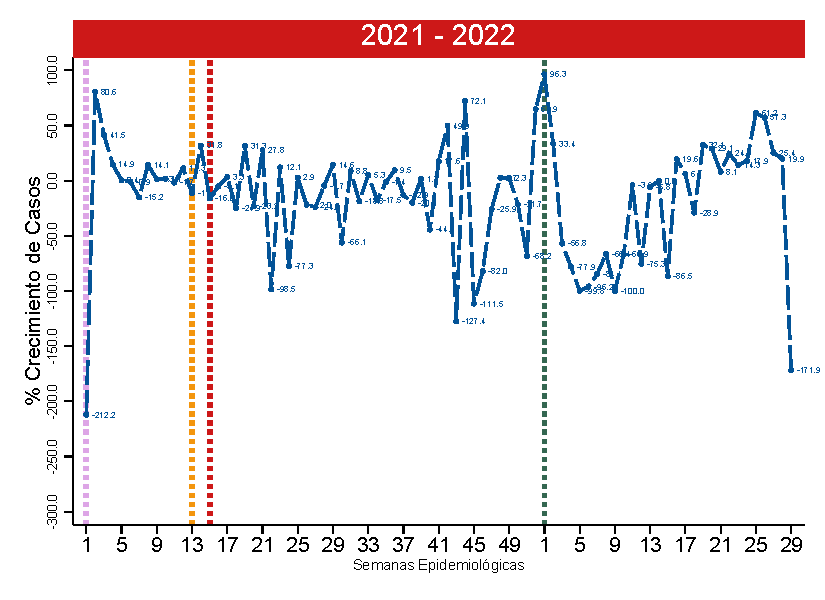
\includegraphics[width=0.9\linewidth]{../figuras/positivos_crecimiento_2021_2022.pdf}
		\end{center} 
		{\tiny Fuente de datos: SISCOVID, NOTICOVID. \\
	Nota:{\color{mycolor1} - -: Año Nuevo}, {\color{mycolor2} - -: Semana Santa}, {\color{mycolor3} - -: Elecciones Primera Vuelta}, {\color{mycolor4} $- \cdot$: Elecciones Segunda Vuelta}, {\color{mycolor7} - -: Año 2022}. \\}
	\end{frame}
	
\begin{frame}
		\frametitle{Tasa de Positividad Semanal por Tipo de Prueba, 2021-2022}
		\vspace{-.5cm}
		\begin{center}
			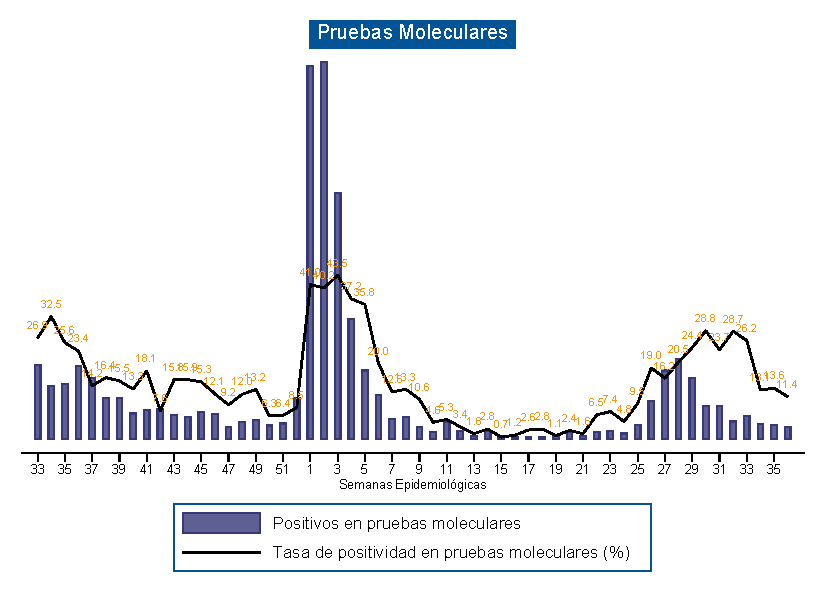
\includegraphics[width=0.8\linewidth]{../figuras/positividad_pcr.pdf}
		\end{center}
		{\tiny Fuente de datos: SISCOVID, NOTICOVID.}
\end{frame}
\begin{frame}
	\frametitle{Tasa de Positividad Semanal por Tipo de Prueba, 2021-2022}
	\vspace{-.5cm}
	\begin{center}
		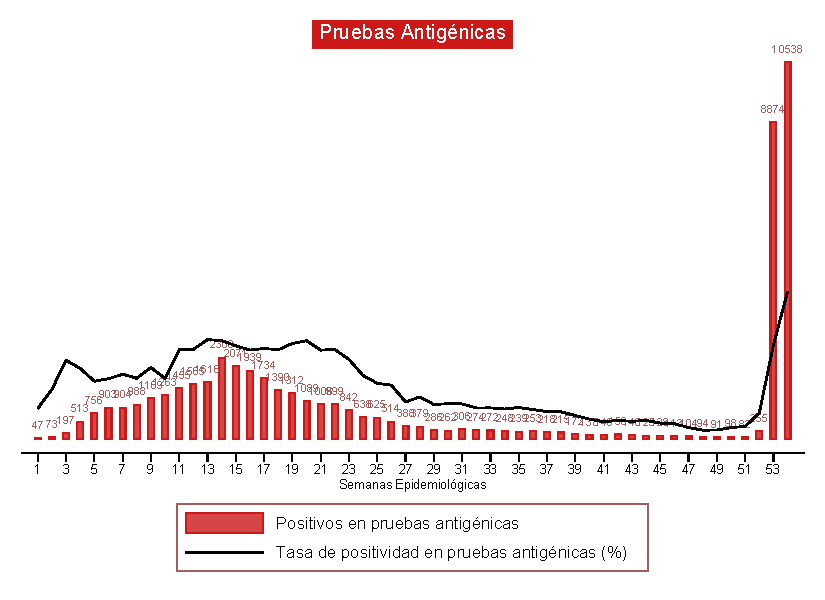
\includegraphics[width=0.8\linewidth]{../figuras/positividad_ag.pdf}
	\end{center}
	{\tiny Fuente de datos: SISCOVID, NOTICOVID.}
\end{frame}

\begin{frame}[label=variantes]
\frametitle{Tendencia de Variantes en la Región Cusco, 2021-2022}
\vspace{-.5cm}
\begin{center}
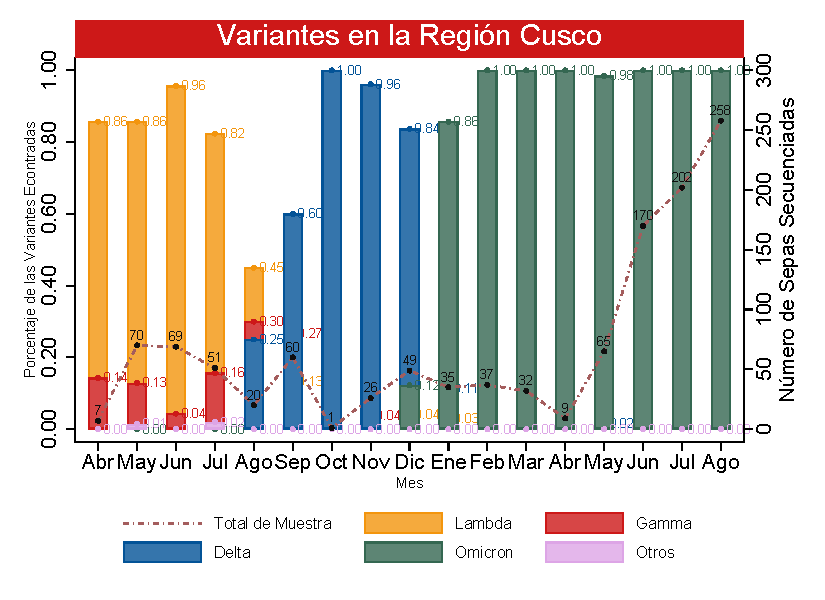
\includegraphics[width=0.9\linewidth]{../figuras/variantes.pdf}
\end{center}
{\tiny Fuente de datos: NETLAB Cusco, UPCH.}
\end{frame}

\begin{frame}[label=mapa_variantes]
\frametitle{Cantidad de Casos Variantes y Dispersión Geográfica en las Provincias de Cusco, 2021-2022}
\begin{center}
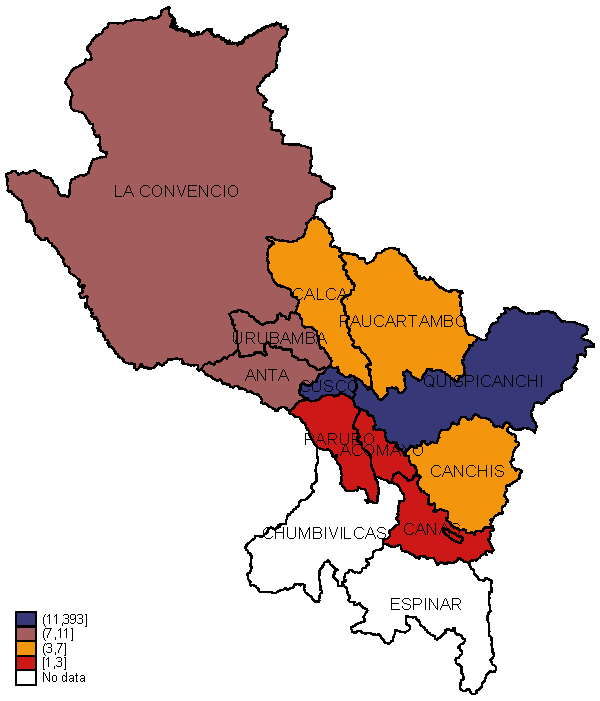
\includegraphics[width=0.4\linewidth]{../figuras/variantes_provincial.pdf}
\end{center}
{\tiny Fuente de datos: NETLAB Cusco, UNSAAC, UPCH.}
	
	Ver detalles para cada  Provincia de Cusco, Distritos de la Región, y por Tipo de variantes haciendo clic en los siguientes enlaces:
	\hyperlink{mapa_provincia_cusco}{\beamergotobutton{Prov. Cusco}} \hyperlink{mapa_distrital}{\beamergotobutton{Distritos de Cusco}} \hyperlink{mapa_lambda}{\beamergotobutton{Lambda}}
	\hyperlink{mapa_gamma}{\beamergotobutton{Gamma}}
	\hyperlink{mapa_delta}{\beamergotobutton{Delta}}
	\hyperlink{mapa_delta}{\beamergotobutton{Omicron}}
\end{frame}

%\begin{frame}
%	\frametitle{Propagación a Nivel Distrital}
%	\vspace{-.5cm}
%	\begin{center}
%		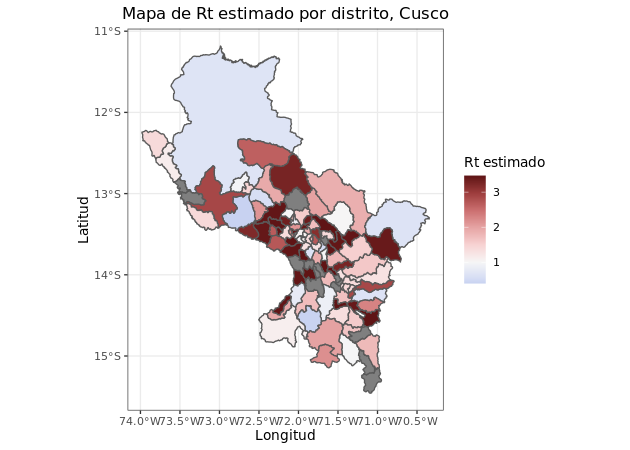
\includegraphics[width=0.75\linewidth, trim={0cm .5cm 0cm 0.2cm},clip]{../sala_nacional/rt_cusco.png}
%	\end{center}
%	{\tiny Fuente: CDC MINSA. Reporte de Vigilancia COVID-19, Perú 2022. Actualización: 2022-03-05. Reporte de número reproductivo efectivo (Rt) de COVID-19. Disponible haciendo clic en el siguiente enlace: \href{https://www.dge.gob.pe/portalnuevo/informacion-publica/reporte-de-numero-reproductivo-efectivo-rt/}{CDC-Rt}. \\}
%	\vspace{0.01cm}
%	$\rightarrow$ Para ver el número exacto de RT por distrito, haga clic en el siguiente link: \href{https://www.dge.gob.pe/portalnuevo/informacion-publica/reporte-de-numero-reproductivo-efectivo-rt/}{\color{mycolor3}reporte-vigilancia-minsa}. \\
%\end{frame}
	
	\begin{frame}
		\frametitle{Defunciones Semanales por COVID-19}
		\vspace{-.5cm}
		\begin{center}
			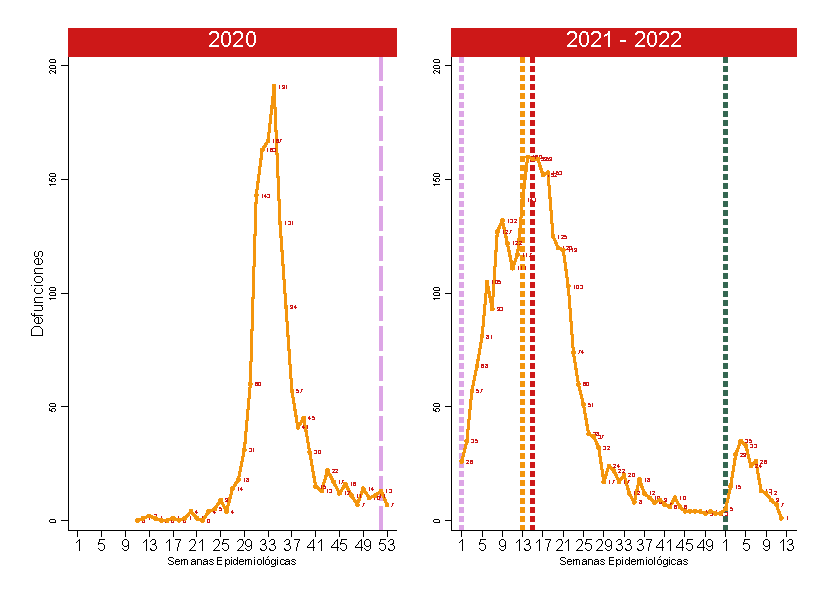
\includegraphics[width=0.9\linewidth, trim={0cm .5cm 0cm 0.2cm},clip]{../figuras/defunciones_semanales_20_21_22.pdf}
		\end{center}
		{\tiny Fuente de datos: SINADEF.\\
		Nota: {\color{mycolor1} --- ---: Navidad}, {\color{mycolor1} - -: Año Nuevo}, {\color{mycolor2} - -: Semana Santa}, {\color{mycolor3} - -: Elecciones Primera Vuelta}, {\color{mycolor4} $- \cdot$: Elecciones Segunda Vuelta},
		{\color{mycolor7} $- \cdot$: Año 2022}. 
	$\rightarrow$ El $86.4\%$ de los fallecidos son mayores de 60 años, siendo el grupo entre 80-89 años la mayoría ($91.4\%$).
	$\rightarrow$ El $2.5\%$ están entre los 0-11 años\\}
	\end{frame}
	
		\begin{frame}
		\frametitle{Promedio diario de Casos y Defunciones}
		\vspace{-.5cm}
		\begin{center}
			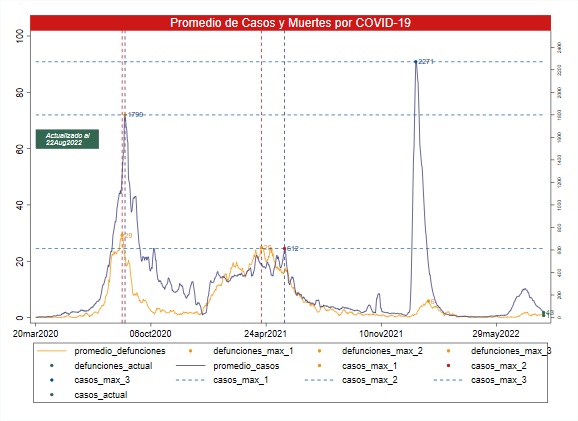
\includegraphics[width=0.9\linewidth, trim={0cm .5cm 0cm 0.2cm},clip]{../figuras/promedio_casos_defuncion_2020_2021_2022.png}
		\end{center}
		{\tiny Fuente de datos: SINADEF - NOTICOVID.}\\
	\end{frame}
	
	\begin{frame}
		\frametitle{Tasa de Crecimiento de Defunciones por Semana}
		\vspace{-.5cm}
		\begin{center}
			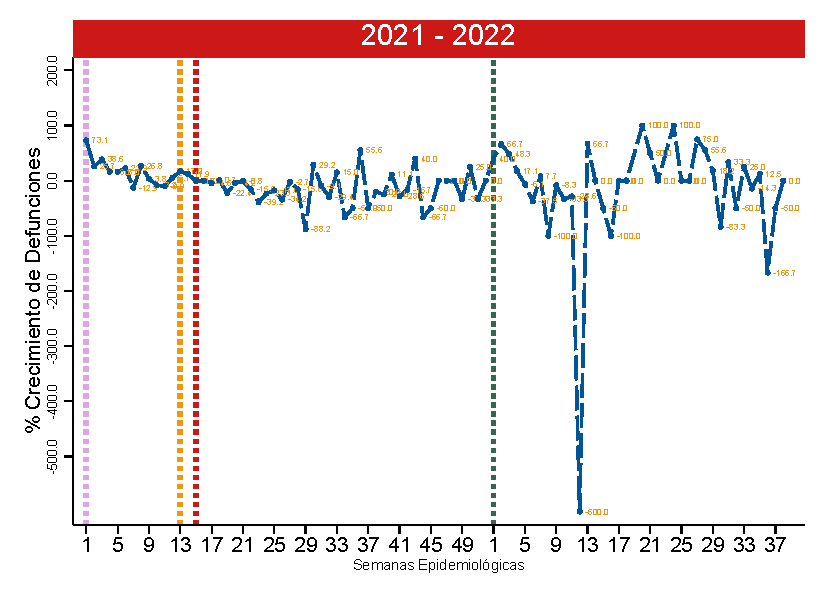
\includegraphics[width=0.9\linewidth]{../figuras/defunciones_tasa_crecimiento_21_22.pdf}
		\end{center} 
		{\tiny Fuente de datos: SINADEF. \\
			Nota: {\color{mycolor1} - -: Año Nuevo}, {\color{mycolor2} - -: Semana Santa}, {\color{mycolor3} - -: Elecciones Primera Vuelta}, {\color{mycolor4} $- \cdot$: Elecciones Segunda Vuelta}, {\color{mycolor7} $- \cdot$: Año 2022}. \\}
	\end{frame}

	\begin{frame}
		\frametitle{Exceso de Defunciones por Todas las Causas}
		\vspace{-.5cm}
		\begin{center}
			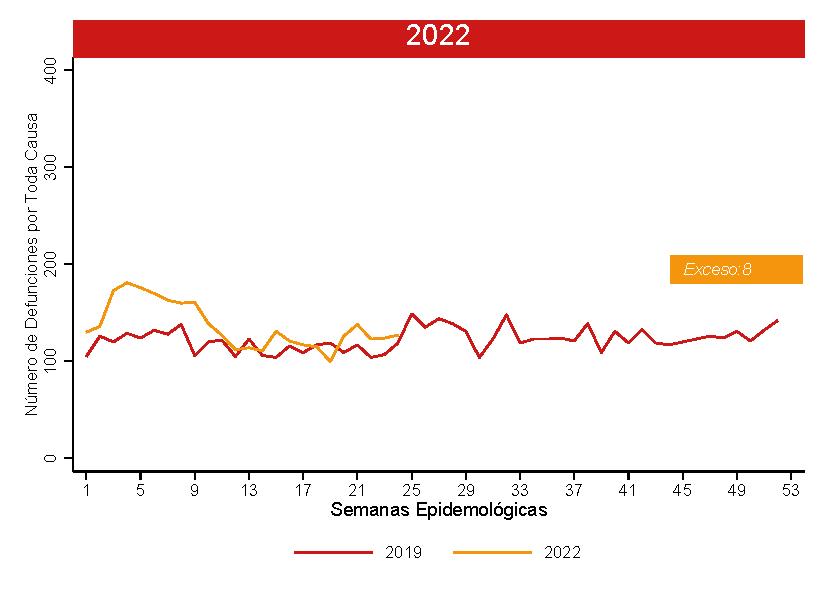
\includegraphics[width=0.9\linewidth]{../figuras/exceso_region_2022.pdf}
		\end{center}
		{\tiny Fuente de datos: SINADEF.} 
	\end{frame}
	
	\begin{frame}
		\frametitle{Mortalidad por Grupos de Edad}
		\vspace{-.1cm}
		\begin{center}
			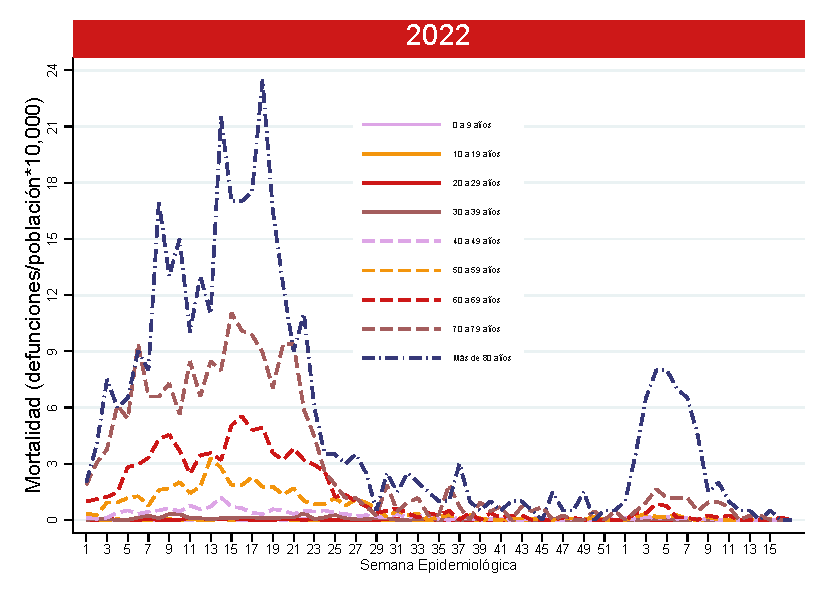
\includegraphics[width=0.9\linewidth]{../figuras/mortalidad_edad_2021_2022.pdf}
		\end{center}
		{\tiny Fuente de datos: SINADEF, Dirección Ejecutiva de Atención Integral de Salud} 
	\end{frame}

\begin{frame}
		\frametitle{Mortalidad por Grupos de Edad (e Hitos de Vacunación)}
	\vspace{.5cm}
\begin{figure}
	\centering
	\begin{subfigure}[b]{0.3\textwidth}
		\centering
		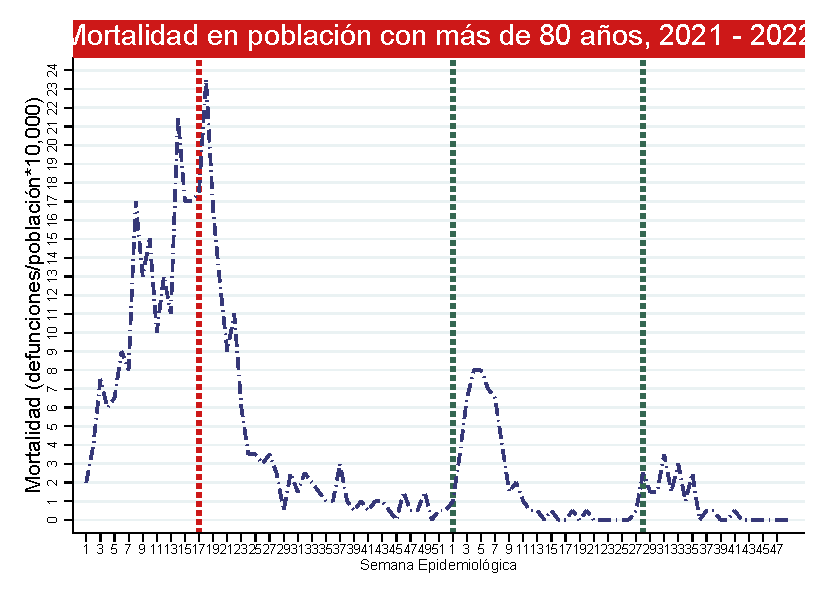
\includegraphics[width=\textwidth]{../figuras/mortalidad_edad_80.pdf}
		\caption{Más de 80 años}
		%\label{fig:}
	\end{subfigure}
	\hfill
	\begin{subfigure}[b]{0.3\textwidth}
		\centering
		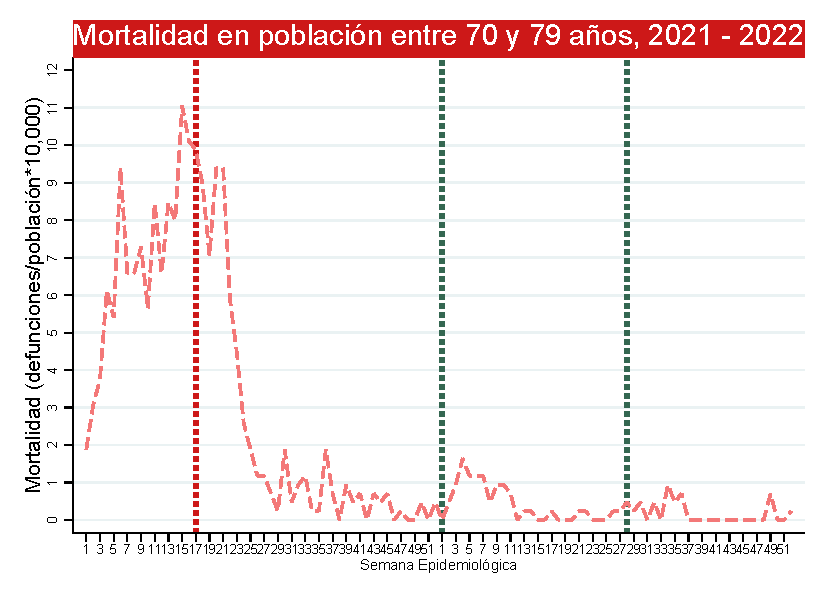
\includegraphics[width=\textwidth]{../figuras/mortalidad_edad_70.pdf}
		\caption{70 a 79 años}
		%\label{fig:70 a 79 años}
	\end{subfigure}
	\hfill
	\begin{subfigure}[b]{0.3\textwidth}
		\centering
		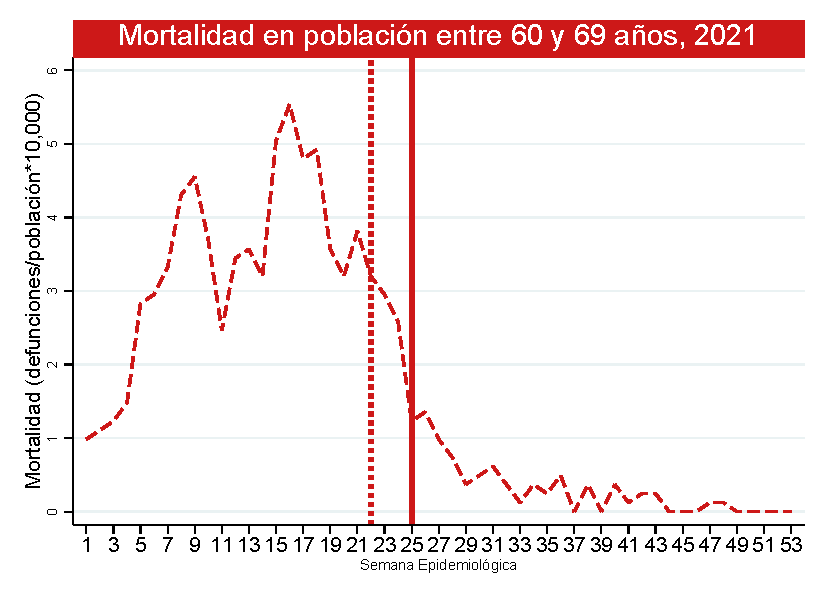
\includegraphics[width=\textwidth]{../figuras/mortalidad_edad_60.pdf}
		\caption{60 a 69 años}
		%\label{fig:60 a 69 años}
	\end{subfigure}
\vspace{10mm}
	\begin{subfigure}[b]{0.3\textwidth}
	\centering
	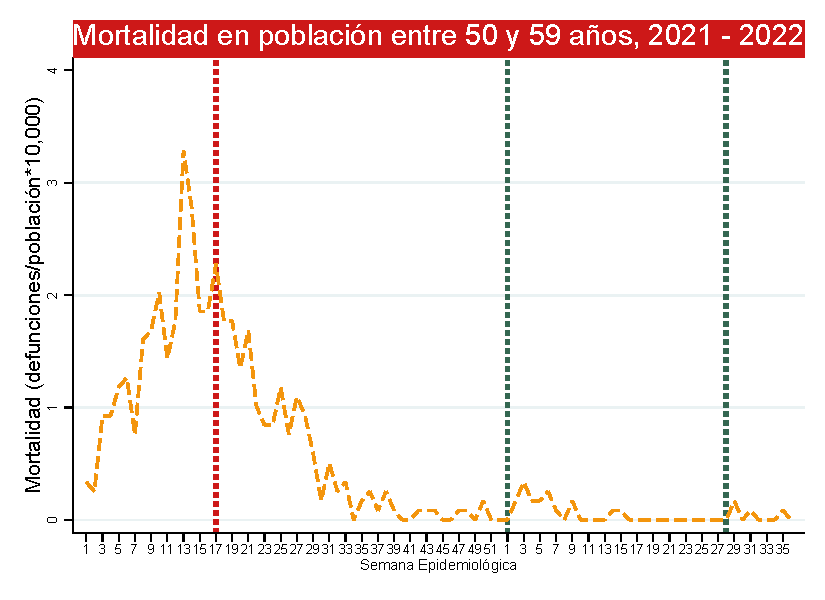
\includegraphics[width=\textwidth]{../figuras/mortalidad_edad_50.pdf}
	\caption{50 a 59 años}
	%\label{fig:50 a 59 años}
\end{subfigure}
	\hfill
\begin{subfigure}[b]{0.3\textwidth}
	\centering
	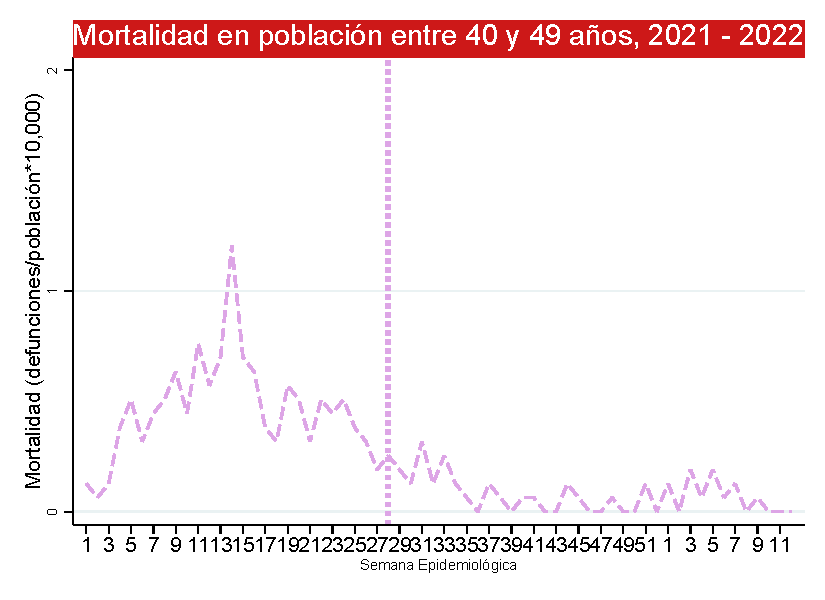
\includegraphics[width=\textwidth]{../figuras/mortalidad_edad_40.pdf}
	\caption{40 a 49 años}
	%\label{fig:40 a 49 años}
\end{subfigure}
\hfill
\begin{subfigure}[b]{0.3\textwidth}
	\centering
	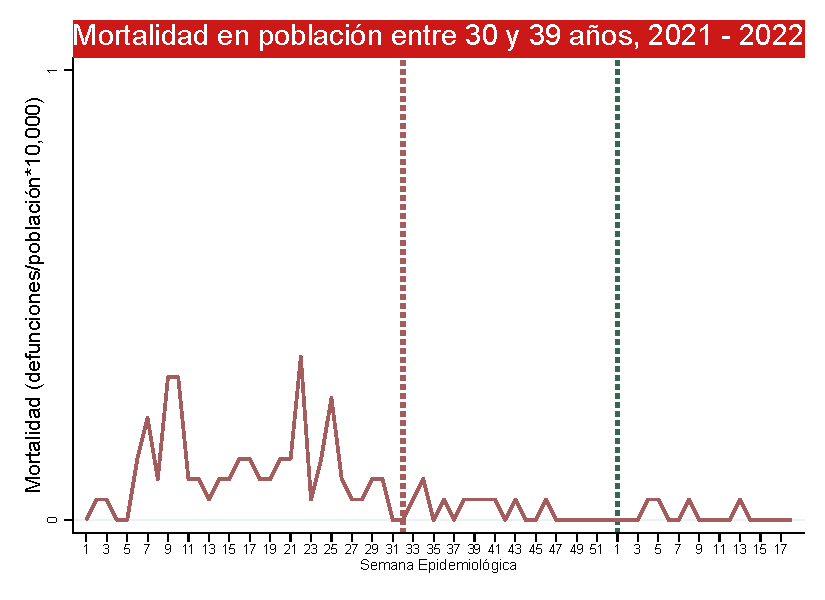
\includegraphics[width=\textwidth]{../figuras/mortalidad_edad_30.pdf}
	\caption{30 a 39 años}
	%\label{fig:40 a 49 años}
\end{subfigure}

	%\caption{Three simple graphs}
	%\label{fig:three graphs}
\end{figure}
\end{frame}

\begin{frame}
	\frametitle{Mortalidad por Grupos de Edad (e Hitos de Vacunación)}
	\vspace{-.2cm}
	\hfill
	\begin{figure}
		\begin{subfigure}[b]{0.3\textwidth}

			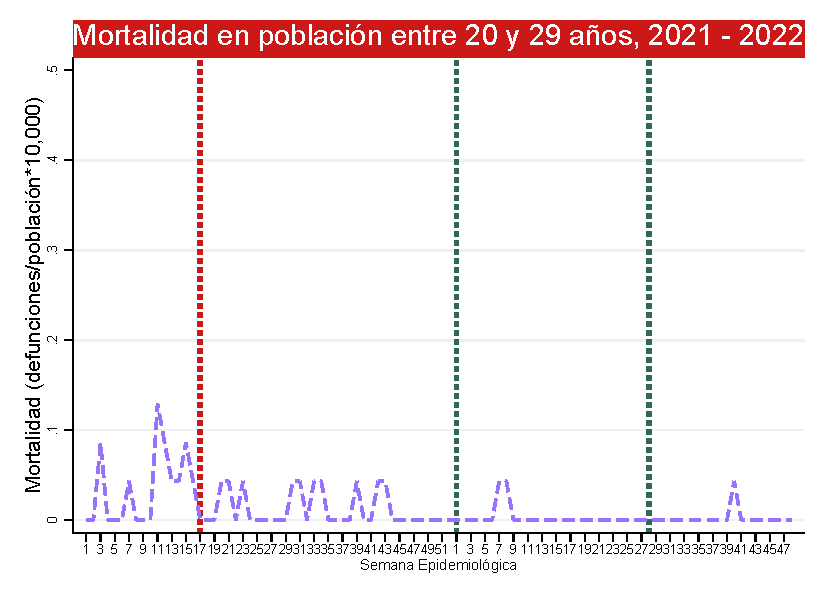
\includegraphics[width=\textwidth]{../figuras/mortalidad_edad_20.pdf}
			\caption{20 a 29 años}
			%\label{fig:}
		\end{subfigure}
		\centering
		\begin{subfigure}[b]{0.3\textwidth}
			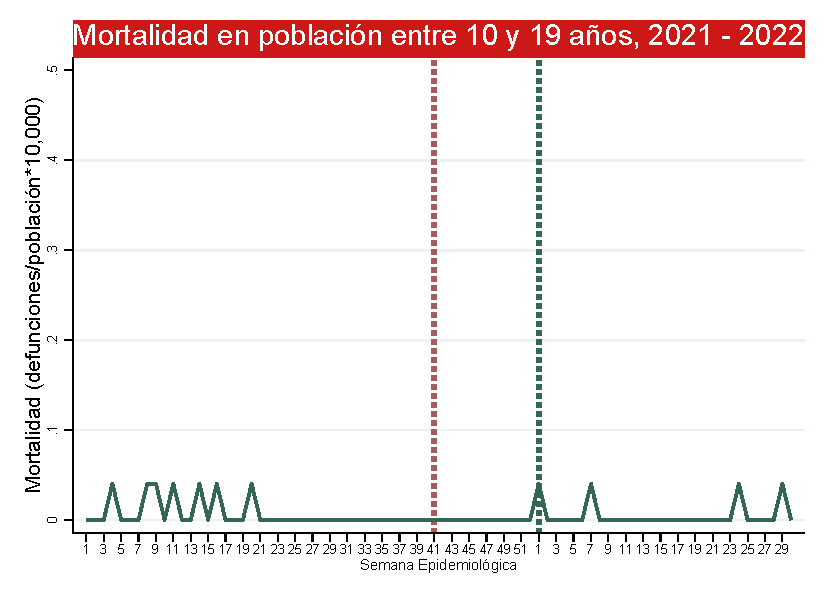
\includegraphics[width=\textwidth]{../figuras/mortalidad_edad_10.pdf}
			\caption{10 a 19 años}
			%\label{fig:70 a 79 años}
		\end{subfigure}
		\begin{subfigure}[b]{0.3\textwidth}

			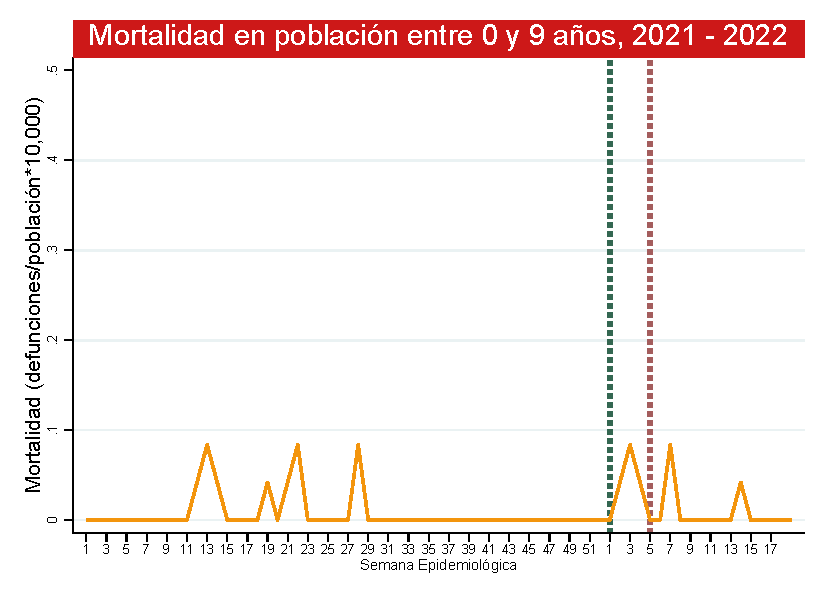
\includegraphics[width=\textwidth]{../figuras/mortalidad_edad_0.pdf}
			\caption{0 a 9 años}
			%\label{fig:60 a 69 años}
		\end{subfigure}
		\vspace{10mm}	
		%\caption{Three simple graphs}
		%\label{fig:three graphs}
	\end{figure}
	\vspace{-.8cm} 
	{\tiny Fuente de datos: SINADEF, Dirección Ejecutiva de Atención Integral de Salud.\\}
	{\tiny Nota: Líneas punteadas (- -) es el inicio de la primera dosis de vacuna contra COVID-19 y línea continua (--) es el inicio de la segunda dosis en el respectivo grupo de edad. Nota 2: Las escalas en el eje y son diferentes.\\}
	$\rightarrow$ {\small La tasa de mortalidad presenta descenso en el número de fallecidos. Se observa que en los grupos etarios que accedieron a la \textbf{\color{mycolor3}vacunación anticipada} presentaron menos número de fallecidos}  \hyperlink{indice}{\beamergotobutton{Índice}}
\end{frame}

\begin{frame}
	\frametitle{Defunciones, tasa de mortalidad y letalidad, Región Cusco, 2020 - 2022}
	\vspace{-1.0cm}
	\begin{table}[]
		\resizebox{\textwidth}{!}{%
				\begin{tabular}{lccc|cccccc|}
		\cline{5-10}
		&
		\multicolumn{1}{l}{} &
		&
		&
		\multicolumn{6}{c|}{\cellcolor[HTML]{F4BFBF}} \\
		&
		\multicolumn{1}{l}{} &
		\multicolumn{1}{l}{} &
		\multicolumn{1}{l|}{} &
		\multicolumn{6}{c|}{\multirow{-2}{*}{\cellcolor[HTML]{F4BFBF}\textbf{Etapa de Vida}}} \\ \cline{5-10} 
		&
		\multicolumn{1}{l}{} &
		\multicolumn{1}{l}{} &
		\multicolumn{1}{l|}{} &
		\multicolumn{1}{c|}{\cellcolor[HTML]{F4BFBF}\textbf{Niño}} &
		\multicolumn{1}{l|}{\cellcolor[HTML]{F4BFBF}\textbf{Adolescente}} &
		\multicolumn{1}{l|}{\cellcolor[HTML]{F4BFBF}\textbf{Joven}} &
		\multicolumn{1}{l|}{\cellcolor[HTML]{F4BFBF}\textbf{Adulto}} &
		\multicolumn{1}{l|}{\cellcolor[HTML]{F4BFBF}\textbf{Adulto Mayor}} &
		\cellcolor[HTML]{F4BFBF}\textbf{Total} \\ \cline{2-10} 
		\multicolumn{1}{l|}{} &
		\multicolumn{1}{c|}{\cellcolor[HTML]{FFD9C0}} &
		\multicolumn{1}{c|}{\cellcolor[HTML]{FFD9C0}} &
		\cellcolor[HTML]{FFD9C0}\textbf{Tasa (\%)} &
		\multicolumn{1}{c|}{\cellcolor[HTML]{FFD9C0}0.4} &
		\multicolumn{1}{c|}{\cellcolor[HTML]{FFD9C0}0.049} &
		\multicolumn{1}{c|}{\cellcolor[HTML]{FFD9C0}0.12} &
		\multicolumn{1}{c|}{\cellcolor[HTML]{FFD9C0}0.57} &
		\multicolumn{1}{c|}{\cellcolor[HTML]{FFD9C0}7.9} &
		\cellcolor[HTML]{FFD9C0}1.3 \\ \cline{4-10} 
		\multicolumn{1}{l|}{} &
		\multicolumn{1}{c|}{\cellcolor[HTML]{FFD9C0}} &
		\multicolumn{1}{c|}{\multirow{-2}{*}{\cellcolor[HTML]{FFD9C0}\textbf{Letalidad}}} &
		\cellcolor[HTML]{FFD9C0} &
		\multicolumn{1}{c|}{\cellcolor[HTML]{FFD9C0}} &
		\multicolumn{1}{c|}{\cellcolor[HTML]{FFD9C0}} &
		\multicolumn{1}{c|}{\cellcolor[HTML]{FFD9C0}} &
		\multicolumn{1}{c|}{\cellcolor[HTML]{FFD9C0}} &
		\multicolumn{1}{c|}{\cellcolor[HTML]{FFD9C0}} &
		\cellcolor[HTML]{FFD9C0} \\ \cline{3-3}
		\multicolumn{1}{l|}{} &
		\multicolumn{1}{c|}{\cellcolor[HTML]{FFD9C0}} &
		\multicolumn{1}{c|}{\cellcolor[HTML]{FFD9C0}} &
		\multirow{-2}{*}{\cellcolor[HTML]{FFD9C0}\textbf{Defunciones}} &
		\multicolumn{1}{c|}{\multirow{-2}{*}{\cellcolor[HTML]{FFD9C0}07}} &
		\multicolumn{1}{c|}{\multirow{-2}{*}{\cellcolor[HTML]{FFD9C0}01}} &
		\multicolumn{1}{c|}{\multirow{-2}{*}{\cellcolor[HTML]{FFD9C0}29}} &
		\multicolumn{1}{c|}{\multirow{-2}{*}{\cellcolor[HTML]{FFD9C0}375}} &
		\multicolumn{1}{c|}{\multirow{-2}{*}{\cellcolor[HTML]{FFD9C0}973}} &
		\multirow{-2}{*}{\cellcolor[HTML]{FFD9C0}1385} \\ \cline{4-10} 
		\multicolumn{1}{l|}{} &
		\multicolumn{1}{c|}{\cellcolor[HTML]{FFD9C0}} &
		\multicolumn{1}{c|}{\multirow{-2}{*}{\cellcolor[HTML]{FFD9C0}\textbf{Mortalidad}}} &
		\cellcolor[HTML]{FFD9C0}\textbf{Tasa*} &
		\multicolumn{1}{c|}{\cellcolor[HTML]{FFD9C0}5.2} &
		\multicolumn{1}{c|}{\cellcolor[HTML]{FFD9C0}0.74} &
		\multicolumn{1}{c|}{\cellcolor[HTML]{FFD9C0}21} &
		\multicolumn{1}{c|}{\cellcolor[HTML]{FFD9C0}276} &
		\multicolumn{1}{c|}{\cellcolor[HTML]{FFD9C0}717} &
		\cellcolor[HTML]{FFD9C0}1020 \\ \cline{3-10} 
		\multicolumn{1}{l|}{} &
		\multicolumn{1}{c|}{\cellcolor[HTML]{FFD9C0}} &
		\multicolumn{1}{c|}{\cellcolor[HTML]{FFD9C0}} &
		\cellcolor[HTML]{FFD9C0}\textbf{Casos +} &
		\multicolumn{1}{c|}{\cellcolor[HTML]{FFD9C0}1749} &
		\multicolumn{1}{c|}{\cellcolor[HTML]{FFD9C0}2029} &
		\multicolumn{1}{c|}{\cellcolor[HTML]{FFD9C0}25091} &
		\multicolumn{1}{c|}{\cellcolor[HTML]{FFD9C0}66024} &
		\multicolumn{1}{c|}{\cellcolor[HTML]{FFD9C0}12255} &
		\cellcolor[HTML]{FFD9C0}107148 \\ \cline{4-10} 
		\multicolumn{1}{l|}{} &
		\multicolumn{1}{c|}{\multirow{-6}{*}{\cellcolor[HTML]{FFD9C0}\textbf{2020}}} &
		\multicolumn{1}{c|}{\multirow{-2}{*}{\cellcolor[HTML]{FFD9C0}\textbf{Incidencia}}} &
		\cellcolor[HTML]{FFD9C0}\textbf{Tasa*} &
		\multicolumn{1}{c|}{\cellcolor[HTML]{FFD9C0}1288} &
		\multicolumn{1}{c|}{\cellcolor[HTML]{FFD9C0}1495} &
		\multicolumn{1}{c|}{\cellcolor[HTML]{FFD9C0}18483} &
		\multicolumn{1}{c|}{\cellcolor[HTML]{FFD9C0}48637} &
		\multicolumn{1}{c|}{\cellcolor[HTML]{FFD9C0}9028} &
		\cellcolor[HTML]{FFD9C0}7.9 \\ \cline{2-10} 
		\multicolumn{1}{l|}{} &
		\multicolumn{1}{c|}{\cellcolor[HTML]{FAF0D7}} &
		\multicolumn{1}{c|}{\cellcolor[HTML]{FAF0D7}} &
		\cellcolor[HTML]{FAF0D7}\textbf{Tasa (\%)} &
		\multicolumn{1}{c|}{\cellcolor[HTML]{FAF0D7}0.94} &
		\multicolumn{1}{c|}{\cellcolor[HTML]{FAF0D7}0.087} &
		\multicolumn{1}{c|}{\cellcolor[HTML]{FAF0D7}0.13} &
		\multicolumn{1}{c|}{\cellcolor[HTML]{FAF0D7}1.9} &
		\multicolumn{1}{c|}{\cellcolor[HTML]{FAF0D7}19} &
		\cellcolor[HTML]{FAF0D7}3.8 \\ \cline{4-10} 
		\multicolumn{1}{l|}{} &
		\multicolumn{1}{c|}{\cellcolor[HTML]{FAF0D7}} &
		\multicolumn{1}{c|}{\multirow{-2}{*}{\cellcolor[HTML]{FAF0D7}\textbf{Letalidad}}} &
		\cellcolor[HTML]{FAF0D7} &
		\multicolumn{1}{c|}{\cellcolor[HTML]{FAF0D7}} &
		\multicolumn{1}{c|}{\cellcolor[HTML]{FAF0D7}} &
		\multicolumn{1}{c|}{\cellcolor[HTML]{FAF0D7}} &
		\multicolumn{1}{c|}{\cellcolor[HTML]{FAF0D7}} &
		\multicolumn{1}{c|}{\cellcolor[HTML]{FAF0D7}} &
		\cellcolor[HTML]{FAF0D7} \\ \cline{3-3}
		\multicolumn{1}{l|}{} &
		\multicolumn{1}{c|}{\cellcolor[HTML]{FAF0D7}} &
		\multicolumn{1}{c|}{\cellcolor[HTML]{FAF0D7}} &
		\multirow{-2}{*}{\cellcolor[HTML]{FAF0D7}\textbf{Defunciones}} &
		\multicolumn{1}{c|}{\multirow{-2}{*}{\cellcolor[HTML]{FAF0D7}11}} &
		\multicolumn{1}{c|}{\multirow{-2}{*}{\cellcolor[HTML]{FAF0D7}04}} &
		\multicolumn{1}{c|}{\multirow{-2}{*}{\cellcolor[HTML]{FAF0D7}25}} &
		\multicolumn{1}{c|}{\multirow{-2}{*}{\cellcolor[HTML]{FAF0D7}826}} &
		\multicolumn{1}{c|}{\multirow{-2}{*}{\cellcolor[HTML]{FAF0D7}2127}} &
		\multirow{-2}{*}{\cellcolor[HTML]{FAF0D7}2993} \\ \cline{4-10} 
		\multicolumn{1}{l|}{} &
		\multicolumn{1}{c|}{\cellcolor[HTML]{FAF0D7}} &
		\multicolumn{1}{c|}{\multirow{-2}{*}{\cellcolor[HTML]{FAF0D7}\textbf{Mortalidad}}} &
		\cellcolor[HTML]{FAF0D7}\textbf{Tasa*} &
		\multicolumn{1}{c|}{\cellcolor[HTML]{FAF0D7}8.1} &
		\multicolumn{1}{c|}{\cellcolor[HTML]{FAF0D7}2.9} &
		\multicolumn{1}{c|}{\cellcolor[HTML]{FAF0D7}18} &
		\multicolumn{1}{c|}{\cellcolor[HTML]{FAF0D7}608} &
		\multicolumn{1}{c|}{\cellcolor[HTML]{FAF0D7}1567} &
		\cellcolor[HTML]{FAF0D7}2205 \\ \cline{3-10} 
		\multicolumn{1}{l|}{} &
		\multicolumn{1}{c|}{\cellcolor[HTML]{FAF0D7}} &
		\multicolumn{1}{c|}{\cellcolor[HTML]{FAF0D7}} &
		\cellcolor[HTML]{FAF0D7}\textbf{Casos +} &
		\multicolumn{1}{c|}{\cellcolor[HTML]{FAF0D7}1173} &
		\multicolumn{1}{c|}{\cellcolor[HTML]{FAF0D7}4573} &
		\multicolumn{1}{c|}{\cellcolor[HTML]{FAF0D7}19526} &
		\multicolumn{1}{c|}{\cellcolor[HTML]{FAF0D7}43215} &
		\multicolumn{1}{c|}{\cellcolor[HTML]{FAF0D7}11129} &
		\cellcolor[HTML]{FAF0D7}79616 \\ \cline{4-10} 
		\multicolumn{1}{l|}{} &
		\multicolumn{1}{c|}{\multirow{-6}{*}{\cellcolor[HTML]{FAF0D7}\textbf{2021}}} &
		\multicolumn{1}{c|}{\multirow{-2}{*}{\cellcolor[HTML]{FAF0D7}\textbf{Incidencia}}} &
		\cellcolor[HTML]{FAF0D7}\textbf{Tasa*} &
		\multicolumn{1}{c|}{\cellcolor[HTML]{FAF0D7}864} &
		\multicolumn{1}{c|}{\cellcolor[HTML]{FAF0D7}3369} &
		\multicolumn{1}{c|}{\cellcolor[HTML]{FAF0D7}14304} &
		\multicolumn{1}{c|}{\cellcolor[HTML]{FAF0D7}31834} &
		\multicolumn{1}{c|}{\cellcolor[HTML]{FAF0D7}8198} &
		\cellcolor[HTML]{FAF0D7}58649 \\ \cline{2-10} 
		\multicolumn{1}{l|}{} &
		\multicolumn{1}{c|}{\cellcolor[HTML]{E2EFDA}} &
		\multicolumn{1}{c|}{\cellcolor[HTML]{E2EFDA}} &
		\cellcolor[HTML]{E2EFDA}\textbf{Tasa(\%)} &
		\multicolumn{1}{c|}{\cellcolor[HTML]{E2EFDA}0.34} &
		\multicolumn{1}{c|}{\cellcolor[HTML]{E2EFDA}0.086} &
		\multicolumn{1}{c|}{\cellcolor[HTML]{E2EFDA}0.033} &
		\multicolumn{1}{c|}{\cellcolor[HTML]{E2EFDA}0.14} &
		\multicolumn{1}{c|}{\cellcolor[HTML]{E2EFDA}3.7} &
		\cellcolor[HTML]{E2EFDA}0.50 \\ \cline{4-10} 
		\multicolumn{1}{l|}{} &
		\multicolumn{1}{c|}{\cellcolor[HTML]{E2EFDA}} &
		\multicolumn{1}{c|}{\multirow{-2}{*}{\cellcolor[HTML]{E2EFDA}\textbf{Letalidad}}} &
		\cellcolor[HTML]{E2EFDA} &
		\multicolumn{1}{c|}{\cellcolor[HTML]{E2EFDA}} &
		\multicolumn{1}{c|}{\cellcolor[HTML]{E2EFDA}} &
		\multicolumn{1}{c|}{\cellcolor[HTML]{E2EFDA}} &
		\multicolumn{1}{c|}{\cellcolor[HTML]{E2EFDA}} &
		\multicolumn{1}{c|}{\cellcolor[HTML]{E2EFDA}} &
		\cellcolor[HTML]{E2EFDA} \\ \cline{3-3}
		\multicolumn{1}{l|}{} &
		\multicolumn{1}{c|}{\cellcolor[HTML]{E2EFDA}} &
		\multicolumn{1}{c|}{\cellcolor[HTML]{E2EFDA}} &
		\multirow{-2}{*}{\cellcolor[HTML]{E2EFDA}\textbf{Defunciones}} &
		\multicolumn{1}{c|}{\multirow{-2}{*}{\cellcolor[HTML]{E2EFDA}08}} &
		\multicolumn{1}{c|}{\multirow{-2}{*}{\cellcolor[HTML]{E2EFDA}02}} &
		\multicolumn{1}{c|}{\multirow{-2}{*}{\cellcolor[HTML]{E2EFDA}05}} &
		\multicolumn{1}{c|}{\multirow{-2}{*}{\cellcolor[HTML]{E2EFDA}41}} &
		\multicolumn{1}{c|}{\multirow{-2}{*}{\cellcolor[HTML]{E2EFDA}225}} &
		\multirow{-2}{*}{\cellcolor[HTML]{E2EFDA}281} \\ \cline{4-10} 
		\multicolumn{1}{l|}{} &
		\multicolumn{1}{c|}{\cellcolor[HTML]{E2EFDA}} &
		\multicolumn{1}{c|}{\multirow{-2}{*}{\cellcolor[HTML]{E2EFDA}\textbf{Mortalidad}}} &
		\cellcolor[HTML]{E2EFDA}\textbf{Tasa *} &
		\multicolumn{1}{c|}{\cellcolor[HTML]{E2EFDA}5.9} &
		\multicolumn{1}{c|}{\cellcolor[HTML]{E2EFDA}1.5} &
		\multicolumn{1}{c|}{\cellcolor[HTML]{E2EFDA}3.7} &
		\multicolumn{1}{c|}{\cellcolor[HTML]{E2EFDA}30} &
		\multicolumn{1}{c|}{\cellcolor[HTML]{E2EFDA}166} &
		\cellcolor[HTML]{E2EFDA}207 \\ \cline{3-10} 
		\multicolumn{1}{l|}{} &
		\multicolumn{1}{c|}{\cellcolor[HTML]{E2EFDA}} &     
		\multicolumn{1}{c|}{\cellcolor[HTML]{E2EFDA}} &
		\cellcolor[HTML]{E2EFDA}\textbf{Casos +} &
		\multicolumn{1}{c|}{\cellcolor[HTML]{E2EFDA}2344} &
		\multicolumn{1}{c|}{\cellcolor[HTML]{E2EFDA}2318} &
		\multicolumn{1}{c|}{\cellcolor[HTML]{E2EFDA}15260} &
		\multicolumn{1}{c|}{\cellcolor[HTML]{E2EFDA}29812} &
		\multicolumn{1}{c|}{\cellcolor[HTML]{E2EFDA}6101} &
		\cellcolor[HTML]{E2EFDA}55835 \\ \cline{4-10} 
		\multicolumn{1}{l|}{} &
		\multicolumn{1}{c|}{\multirow{-6}{*}{\cellcolor[HTML]{E2EFDA}\textbf{2022}}} &
		\multicolumn{1}{c|}{\multirow{-2}{*}{\cellcolor[HTML]{E2EFDA}\textbf{Incidencia}}} &
		\cellcolor[HTML]{E2EFDA}\textbf{Tasa} &
		\multicolumn{1}{c|}{\cellcolor[HTML]{E2EFDA}1727} &
		\multicolumn{1}{c|}{\cellcolor[HTML]{E2EFDA}1708} &
		\multicolumn{1}{c|}{\cellcolor[HTML]{E2EFDA}11241} &
		\multicolumn{1}{c|}{\cellcolor[HTML]{E2EFDA}21961} &
		\multicolumn{1}{c|}{\cellcolor[HTML]{E2EFDA}4494} &
		\cellcolor[HTML]{E2EFDA}41131 \\ \cline{2-10} 	
	\end{tabular}
		}
	\end{table}	
	{   \tiny Fuente de datos: NOTICOVID, SISCOVID, SINADEF.\\
		Tasa de mortalidad ajustada 1 000 000 de habitantes*.\\
		Tasa de incidencia ajustada 1 000 000 de habitantes*.\\ 
	}
	
\end{frame}

%\begin{frame}
%	\frametitle{Tabla por Casos y Tasa de Incidencia Perú, 2020 - 2022}
%	\vspace{-.5cm}
%	\begin{table}[]
%		\resizebox{\textwidth}{!}{%
%				\begin{tabular}{lcccccc}
		\multicolumn{7}{c}{Defunciones y tasa de letalidad por cursos de vida, Perú 2020-2022} \\
		&\multicolumn{2}{c}{\cellcolor[HTML]{303498}{\color[HTML]{EFEFEF}\textbf{2020}}}     
		&\multicolumn{2}{c}{\cellcolor[HTML]{303498}{\color[HTML]{EFEFEF}\textbf{2021}}}      
		&\multicolumn{2}{c}{\cellcolor[HTML]{303498}{\color[HTML]{EFEFEF}\textbf{2022}}}\\
		\rowcolor[HTML]{303498} 
		\multicolumn{1}{c}{\cellcolor[HTML]{303498}{\color[HTML]{FFFFFF} \textbf {Curso de vida}}} 
		&{\color[HTML]{FFFFFF} {Defunciones}} 
		&{\color[HTML]{FFFFFF} {Tasa de letalidad}} 
		&{\color[HTML]{FFFFFF} {Defunciones}} 
		&{\color[HTML]{FFFFFF} {Tasa de letalidad}} 
		&{\color[HTML]{FFFFFF} {Defunciones}} 
		&{\color[HTML]{FFFFFF} {Tasa de letalidad}} \\
		Niño                                                                             
		&501                               & 1,2                                      
		&334                               & 1,1                                      
		&115                               & 0,3 \\
		Adolescente                                                                      
		&180                               & 0,6                                      
		&168                               & 0,4                                      
		&34                                & 0,1 \\
		Joven                                                                            
		&1285                              & 0,6                                      
		&1258                              & 0,4                                      
		&176                               & 0,1 \\
		Adulto                                                                           
		&25529                             & 4,1                                      
		&33105                             & 4,5                                      
		&1377                              & 0,2 \\
		Adulto Mayor                                                                     
		&67302                             & 35,1                                     
		&73871                             & 35,2                                     
		&6516                              & 3,4  \\
		\rowcolor[HTML]{303498} 
		\multicolumn{1}{c}{\cellcolor[HTML]{303498}{\color[HTML]{FFFFFF} Total}}         
		&{\color[HTML]{FFFFFF} 94 797}      & {\color[HTML]{FFFFFF} 8,6}               
		&{\color[HTML]{FFFFFF} 108736}      & {\color[HTML]{FFFFFF} 8,2}               
		&{\color[HTML]{FFFFFF} 8218}        & {\color[HTML]{FFFFFF} 0,7}              
	\end{tabular}


%		}
%	\end{table}	
%	{\tiny Fuente de datos: SISCOVID, NOTICOVID.}
%	
%\end{frame}
%
%\begin{frame}
%	\frametitle{Tabla por Defunciones y Tasa de Mortalidad Perú, 2020 - 2022}
%	\vspace{-.5cm}
%	
%	\begin{table}[]
%		\resizebox{\textwidth}{!}{%
%				\begin{tabular}{lccc|cccccc|}
		\cline{5-10}
		&
		\multicolumn{1}{l}{} &
		&
		&
		\multicolumn{6}{c|}{\cellcolor[HTML]{F4BFBF}} \\
		&
		\multicolumn{1}{l}{} &
		\multicolumn{1}{l}{} &
		\multicolumn{1}{l|}{} &
		\multicolumn{6}{c|}{\multirow{-2}{*}{\cellcolor[HTML]{F4BFBF}\textbf{Etapa de Vida}}} \\ \cline{5-10} 
		&
		\multicolumn{1}{l}{} &
		\multicolumn{1}{l}{} &
		\multicolumn{1}{l|}{} &
		\multicolumn{1}{c|}{\cellcolor[HTML]{F4BFBF}\textbf{Niño}} &
		\multicolumn{1}{l|}{\cellcolor[HTML]{F4BFBF}\textbf{Adolescente}} &
		\multicolumn{1}{l|}{\cellcolor[HTML]{F4BFBF}\textbf{Joven}} &
		\multicolumn{1}{l|}{\cellcolor[HTML]{F4BFBF}\textbf{Adulto}} &
		\multicolumn{1}{l|}{\cellcolor[HTML]{F4BFBF}\textbf{Adulto Mayor}} &
		\cellcolor[HTML]{F4BFBF}\textbf{Total} \\ \cline{2-10} 
		\multicolumn{1}{l|}{} &
		\multicolumn{1}{c|}{\cellcolor[HTML]{FFD9C0}} &
		\multicolumn{1}{c|}{\cellcolor[HTML]{FFD9C0}} &
		\cellcolor[HTML]{FFD9C0}\textbf{Tasa (\%)} &
		\multicolumn{1}{c|}{\cellcolor[HTML]{FFD9C0}0.4} &
		\multicolumn{1}{c|}{\cellcolor[HTML]{FFD9C0}0.049} &
		\multicolumn{1}{c|}{\cellcolor[HTML]{FFD9C0}0.12} &
		\multicolumn{1}{c|}{\cellcolor[HTML]{FFD9C0}0.57} &
		\multicolumn{1}{c|}{\cellcolor[HTML]{FFD9C0}7.9} &
		\cellcolor[HTML]{FFD9C0}1.3 \\ \cline{4-10} 
		\multicolumn{1}{l|}{} &
		\multicolumn{1}{c|}{\cellcolor[HTML]{FFD9C0}} &
		\multicolumn{1}{c|}{\multirow{-2}{*}{\cellcolor[HTML]{FFD9C0}\textbf{Letalidad}}} &
		\cellcolor[HTML]{FFD9C0} &
		\multicolumn{1}{c|}{\cellcolor[HTML]{FFD9C0}} &
		\multicolumn{1}{c|}{\cellcolor[HTML]{FFD9C0}} &
		\multicolumn{1}{c|}{\cellcolor[HTML]{FFD9C0}} &
		\multicolumn{1}{c|}{\cellcolor[HTML]{FFD9C0}} &
		\multicolumn{1}{c|}{\cellcolor[HTML]{FFD9C0}} &
		\cellcolor[HTML]{FFD9C0} \\ \cline{3-3}
		\multicolumn{1}{l|}{} &
		\multicolumn{1}{c|}{\cellcolor[HTML]{FFD9C0}} &
		\multicolumn{1}{c|}{\cellcolor[HTML]{FFD9C0}} &
		\multirow{-2}{*}{\cellcolor[HTML]{FFD9C0}\textbf{Defunciones}} &
		\multicolumn{1}{c|}{\multirow{-2}{*}{\cellcolor[HTML]{FFD9C0}07}} &
		\multicolumn{1}{c|}{\multirow{-2}{*}{\cellcolor[HTML]{FFD9C0}01}} &
		\multicolumn{1}{c|}{\multirow{-2}{*}{\cellcolor[HTML]{FFD9C0}29}} &
		\multicolumn{1}{c|}{\multirow{-2}{*}{\cellcolor[HTML]{FFD9C0}375}} &
		\multicolumn{1}{c|}{\multirow{-2}{*}{\cellcolor[HTML]{FFD9C0}973}} &
		\multirow{-2}{*}{\cellcolor[HTML]{FFD9C0}1385} \\ \cline{4-10} 
		\multicolumn{1}{l|}{} &
		\multicolumn{1}{c|}{\cellcolor[HTML]{FFD9C0}} &
		\multicolumn{1}{c|}{\multirow{-2}{*}{\cellcolor[HTML]{FFD9C0}\textbf{Mortalidad}}} &
		\cellcolor[HTML]{FFD9C0}\textbf{Tasa*} &
		\multicolumn{1}{c|}{\cellcolor[HTML]{FFD9C0}5.2} &
		\multicolumn{1}{c|}{\cellcolor[HTML]{FFD9C0}0.74} &
		\multicolumn{1}{c|}{\cellcolor[HTML]{FFD9C0}21} &
		\multicolumn{1}{c|}{\cellcolor[HTML]{FFD9C0}276} &
		\multicolumn{1}{c|}{\cellcolor[HTML]{FFD9C0}717} &
		\cellcolor[HTML]{FFD9C0}1020 \\ \cline{3-10} 
		\multicolumn{1}{l|}{} &
		\multicolumn{1}{c|}{\cellcolor[HTML]{FFD9C0}} &
		\multicolumn{1}{c|}{\cellcolor[HTML]{FFD9C0}} &
		\cellcolor[HTML]{FFD9C0}\textbf{Casos +} &
		\multicolumn{1}{c|}{\cellcolor[HTML]{FFD9C0}1749} &
		\multicolumn{1}{c|}{\cellcolor[HTML]{FFD9C0}2029} &
		\multicolumn{1}{c|}{\cellcolor[HTML]{FFD9C0}25091} &
		\multicolumn{1}{c|}{\cellcolor[HTML]{FFD9C0}66024} &
		\multicolumn{1}{c|}{\cellcolor[HTML]{FFD9C0}12255} &
		\cellcolor[HTML]{FFD9C0}107148 \\ \cline{4-10} 
		\multicolumn{1}{l|}{} &
		\multicolumn{1}{c|}{\multirow{-6}{*}{\cellcolor[HTML]{FFD9C0}\textbf{2020}}} &
		\multicolumn{1}{c|}{\multirow{-2}{*}{\cellcolor[HTML]{FFD9C0}\textbf{Incidencia}}} &
		\cellcolor[HTML]{FFD9C0}\textbf{Tasa*} &
		\multicolumn{1}{c|}{\cellcolor[HTML]{FFD9C0}1288} &
		\multicolumn{1}{c|}{\cellcolor[HTML]{FFD9C0}1495} &
		\multicolumn{1}{c|}{\cellcolor[HTML]{FFD9C0}18483} &
		\multicolumn{1}{c|}{\cellcolor[HTML]{FFD9C0}48637} &
		\multicolumn{1}{c|}{\cellcolor[HTML]{FFD9C0}9028} &
		\cellcolor[HTML]{FFD9C0}7.9 \\ \cline{2-10} 
		\multicolumn{1}{l|}{} &
		\multicolumn{1}{c|}{\cellcolor[HTML]{FAF0D7}} &
		\multicolumn{1}{c|}{\cellcolor[HTML]{FAF0D7}} &
		\cellcolor[HTML]{FAF0D7}\textbf{Tasa (\%)} &
		\multicolumn{1}{c|}{\cellcolor[HTML]{FAF0D7}0.94} &
		\multicolumn{1}{c|}{\cellcolor[HTML]{FAF0D7}0.087} &
		\multicolumn{1}{c|}{\cellcolor[HTML]{FAF0D7}0.13} &
		\multicolumn{1}{c|}{\cellcolor[HTML]{FAF0D7}1.9} &
		\multicolumn{1}{c|}{\cellcolor[HTML]{FAF0D7}19} &
		\cellcolor[HTML]{FAF0D7}3.8 \\ \cline{4-10} 
		\multicolumn{1}{l|}{} &
		\multicolumn{1}{c|}{\cellcolor[HTML]{FAF0D7}} &
		\multicolumn{1}{c|}{\multirow{-2}{*}{\cellcolor[HTML]{FAF0D7}\textbf{Letalidad}}} &
		\cellcolor[HTML]{FAF0D7} &
		\multicolumn{1}{c|}{\cellcolor[HTML]{FAF0D7}} &
		\multicolumn{1}{c|}{\cellcolor[HTML]{FAF0D7}} &
		\multicolumn{1}{c|}{\cellcolor[HTML]{FAF0D7}} &
		\multicolumn{1}{c|}{\cellcolor[HTML]{FAF0D7}} &
		\multicolumn{1}{c|}{\cellcolor[HTML]{FAF0D7}} &
		\cellcolor[HTML]{FAF0D7} \\ \cline{3-3}
		\multicolumn{1}{l|}{} &
		\multicolumn{1}{c|}{\cellcolor[HTML]{FAF0D7}} &
		\multicolumn{1}{c|}{\cellcolor[HTML]{FAF0D7}} &
		\multirow{-2}{*}{\cellcolor[HTML]{FAF0D7}\textbf{Defunciones}} &
		\multicolumn{1}{c|}{\multirow{-2}{*}{\cellcolor[HTML]{FAF0D7}11}} &
		\multicolumn{1}{c|}{\multirow{-2}{*}{\cellcolor[HTML]{FAF0D7}04}} &
		\multicolumn{1}{c|}{\multirow{-2}{*}{\cellcolor[HTML]{FAF0D7}25}} &
		\multicolumn{1}{c|}{\multirow{-2}{*}{\cellcolor[HTML]{FAF0D7}826}} &
		\multicolumn{1}{c|}{\multirow{-2}{*}{\cellcolor[HTML]{FAF0D7}2127}} &
		\multirow{-2}{*}{\cellcolor[HTML]{FAF0D7}2993} \\ \cline{4-10} 
		\multicolumn{1}{l|}{} &
		\multicolumn{1}{c|}{\cellcolor[HTML]{FAF0D7}} &
		\multicolumn{1}{c|}{\multirow{-2}{*}{\cellcolor[HTML]{FAF0D7}\textbf{Mortalidad}}} &
		\cellcolor[HTML]{FAF0D7}\textbf{Tasa*} &
		\multicolumn{1}{c|}{\cellcolor[HTML]{FAF0D7}8.1} &
		\multicolumn{1}{c|}{\cellcolor[HTML]{FAF0D7}2.9} &
		\multicolumn{1}{c|}{\cellcolor[HTML]{FAF0D7}18} &
		\multicolumn{1}{c|}{\cellcolor[HTML]{FAF0D7}608} &
		\multicolumn{1}{c|}{\cellcolor[HTML]{FAF0D7}1567} &
		\cellcolor[HTML]{FAF0D7}2205 \\ \cline{3-10} 
		\multicolumn{1}{l|}{} &
		\multicolumn{1}{c|}{\cellcolor[HTML]{FAF0D7}} &
		\multicolumn{1}{c|}{\cellcolor[HTML]{FAF0D7}} &
		\cellcolor[HTML]{FAF0D7}\textbf{Casos +} &
		\multicolumn{1}{c|}{\cellcolor[HTML]{FAF0D7}1173} &
		\multicolumn{1}{c|}{\cellcolor[HTML]{FAF0D7}4573} &
		\multicolumn{1}{c|}{\cellcolor[HTML]{FAF0D7}19526} &
		\multicolumn{1}{c|}{\cellcolor[HTML]{FAF0D7}43215} &
		\multicolumn{1}{c|}{\cellcolor[HTML]{FAF0D7}11129} &
		\cellcolor[HTML]{FAF0D7}79616 \\ \cline{4-10} 
		\multicolumn{1}{l|}{} &
		\multicolumn{1}{c|}{\multirow{-6}{*}{\cellcolor[HTML]{FAF0D7}\textbf{2021}}} &
		\multicolumn{1}{c|}{\multirow{-2}{*}{\cellcolor[HTML]{FAF0D7}\textbf{Incidencia}}} &
		\cellcolor[HTML]{FAF0D7}\textbf{Tasa*} &
		\multicolumn{1}{c|}{\cellcolor[HTML]{FAF0D7}864} &
		\multicolumn{1}{c|}{\cellcolor[HTML]{FAF0D7}3369} &
		\multicolumn{1}{c|}{\cellcolor[HTML]{FAF0D7}14304} &
		\multicolumn{1}{c|}{\cellcolor[HTML]{FAF0D7}31834} &
		\multicolumn{1}{c|}{\cellcolor[HTML]{FAF0D7}8198} &
		\cellcolor[HTML]{FAF0D7}58649 \\ \cline{2-10} 
		\multicolumn{1}{l|}{} &
		\multicolumn{1}{c|}{\cellcolor[HTML]{E2EFDA}} &
		\multicolumn{1}{c|}{\cellcolor[HTML]{E2EFDA}} &
		\cellcolor[HTML]{E2EFDA}\textbf{Tasa(\%)} &
		\multicolumn{1}{c|}{\cellcolor[HTML]{E2EFDA}0.34} &
		\multicolumn{1}{c|}{\cellcolor[HTML]{E2EFDA}0.086} &
		\multicolumn{1}{c|}{\cellcolor[HTML]{E2EFDA}0.033} &
		\multicolumn{1}{c|}{\cellcolor[HTML]{E2EFDA}0.14} &
		\multicolumn{1}{c|}{\cellcolor[HTML]{E2EFDA}3.7} &
		\cellcolor[HTML]{E2EFDA}0.50 \\ \cline{4-10} 
		\multicolumn{1}{l|}{} &
		\multicolumn{1}{c|}{\cellcolor[HTML]{E2EFDA}} &
		\multicolumn{1}{c|}{\multirow{-2}{*}{\cellcolor[HTML]{E2EFDA}\textbf{Letalidad}}} &
		\cellcolor[HTML]{E2EFDA} &
		\multicolumn{1}{c|}{\cellcolor[HTML]{E2EFDA}} &
		\multicolumn{1}{c|}{\cellcolor[HTML]{E2EFDA}} &
		\multicolumn{1}{c|}{\cellcolor[HTML]{E2EFDA}} &
		\multicolumn{1}{c|}{\cellcolor[HTML]{E2EFDA}} &
		\multicolumn{1}{c|}{\cellcolor[HTML]{E2EFDA}} &
		\cellcolor[HTML]{E2EFDA} \\ \cline{3-3}
		\multicolumn{1}{l|}{} &
		\multicolumn{1}{c|}{\cellcolor[HTML]{E2EFDA}} &
		\multicolumn{1}{c|}{\cellcolor[HTML]{E2EFDA}} &
		\multirow{-2}{*}{\cellcolor[HTML]{E2EFDA}\textbf{Defunciones}} &
		\multicolumn{1}{c|}{\multirow{-2}{*}{\cellcolor[HTML]{E2EFDA}08}} &
		\multicolumn{1}{c|}{\multirow{-2}{*}{\cellcolor[HTML]{E2EFDA}02}} &
		\multicolumn{1}{c|}{\multirow{-2}{*}{\cellcolor[HTML]{E2EFDA}05}} &
		\multicolumn{1}{c|}{\multirow{-2}{*}{\cellcolor[HTML]{E2EFDA}41}} &
		\multicolumn{1}{c|}{\multirow{-2}{*}{\cellcolor[HTML]{E2EFDA}225}} &
		\multirow{-2}{*}{\cellcolor[HTML]{E2EFDA}281} \\ \cline{4-10} 
		\multicolumn{1}{l|}{} &
		\multicolumn{1}{c|}{\cellcolor[HTML]{E2EFDA}} &
		\multicolumn{1}{c|}{\multirow{-2}{*}{\cellcolor[HTML]{E2EFDA}\textbf{Mortalidad}}} &
		\cellcolor[HTML]{E2EFDA}\textbf{Tasa *} &
		\multicolumn{1}{c|}{\cellcolor[HTML]{E2EFDA}5.9} &
		\multicolumn{1}{c|}{\cellcolor[HTML]{E2EFDA}1.5} &
		\multicolumn{1}{c|}{\cellcolor[HTML]{E2EFDA}3.7} &
		\multicolumn{1}{c|}{\cellcolor[HTML]{E2EFDA}30} &
		\multicolumn{1}{c|}{\cellcolor[HTML]{E2EFDA}166} &
		\cellcolor[HTML]{E2EFDA}207 \\ \cline{3-10} 
		\multicolumn{1}{l|}{} &
		\multicolumn{1}{c|}{\cellcolor[HTML]{E2EFDA}} &     
		\multicolumn{1}{c|}{\cellcolor[HTML]{E2EFDA}} &
		\cellcolor[HTML]{E2EFDA}\textbf{Casos +} &
		\multicolumn{1}{c|}{\cellcolor[HTML]{E2EFDA}2344} &
		\multicolumn{1}{c|}{\cellcolor[HTML]{E2EFDA}2318} &
		\multicolumn{1}{c|}{\cellcolor[HTML]{E2EFDA}15260} &
		\multicolumn{1}{c|}{\cellcolor[HTML]{E2EFDA}29812} &
		\multicolumn{1}{c|}{\cellcolor[HTML]{E2EFDA}6101} &
		\cellcolor[HTML]{E2EFDA}55835 \\ \cline{4-10} 
		\multicolumn{1}{l|}{} &
		\multicolumn{1}{c|}{\multirow{-6}{*}{\cellcolor[HTML]{E2EFDA}\textbf{2022}}} &
		\multicolumn{1}{c|}{\multirow{-2}{*}{\cellcolor[HTML]{E2EFDA}\textbf{Incidencia}}} &
		\cellcolor[HTML]{E2EFDA}\textbf{Tasa} &
		\multicolumn{1}{c|}{\cellcolor[HTML]{E2EFDA}1727} &
		\multicolumn{1}{c|}{\cellcolor[HTML]{E2EFDA}1708} &
		\multicolumn{1}{c|}{\cellcolor[HTML]{E2EFDA}11241} &
		\multicolumn{1}{c|}{\cellcolor[HTML]{E2EFDA}21961} &
		\multicolumn{1}{c|}{\cellcolor[HTML]{E2EFDA}4494} &
		\cellcolor[HTML]{E2EFDA}41131 \\ \cline{2-10} 	
	\end{tabular}
%		}
%	\end{table}	
%	{\tiny Fuente de datos: SISCOVID, NOTICOVID.}
%	
%\end{frame}
%------------------------------------------------------------------------------------------------------------------------------------------------------------------------------------------------------------------------------------------
% SECCIÓN 2: Indicadores Epidemiológicos, Región Cusco
%------------------------------------------------------------------------------------------------------------------------------------------------------------------------------------------------------------------------------------------

\section{Cobertura de Vacunación, Región Cusco}

\begin{frame}[label=cobertura_vacuna]
	\frametitle{Cobertura de Vacunación por Provincias, Región Cusco}
	\vspace{-.7cm}
	\begin{center}
		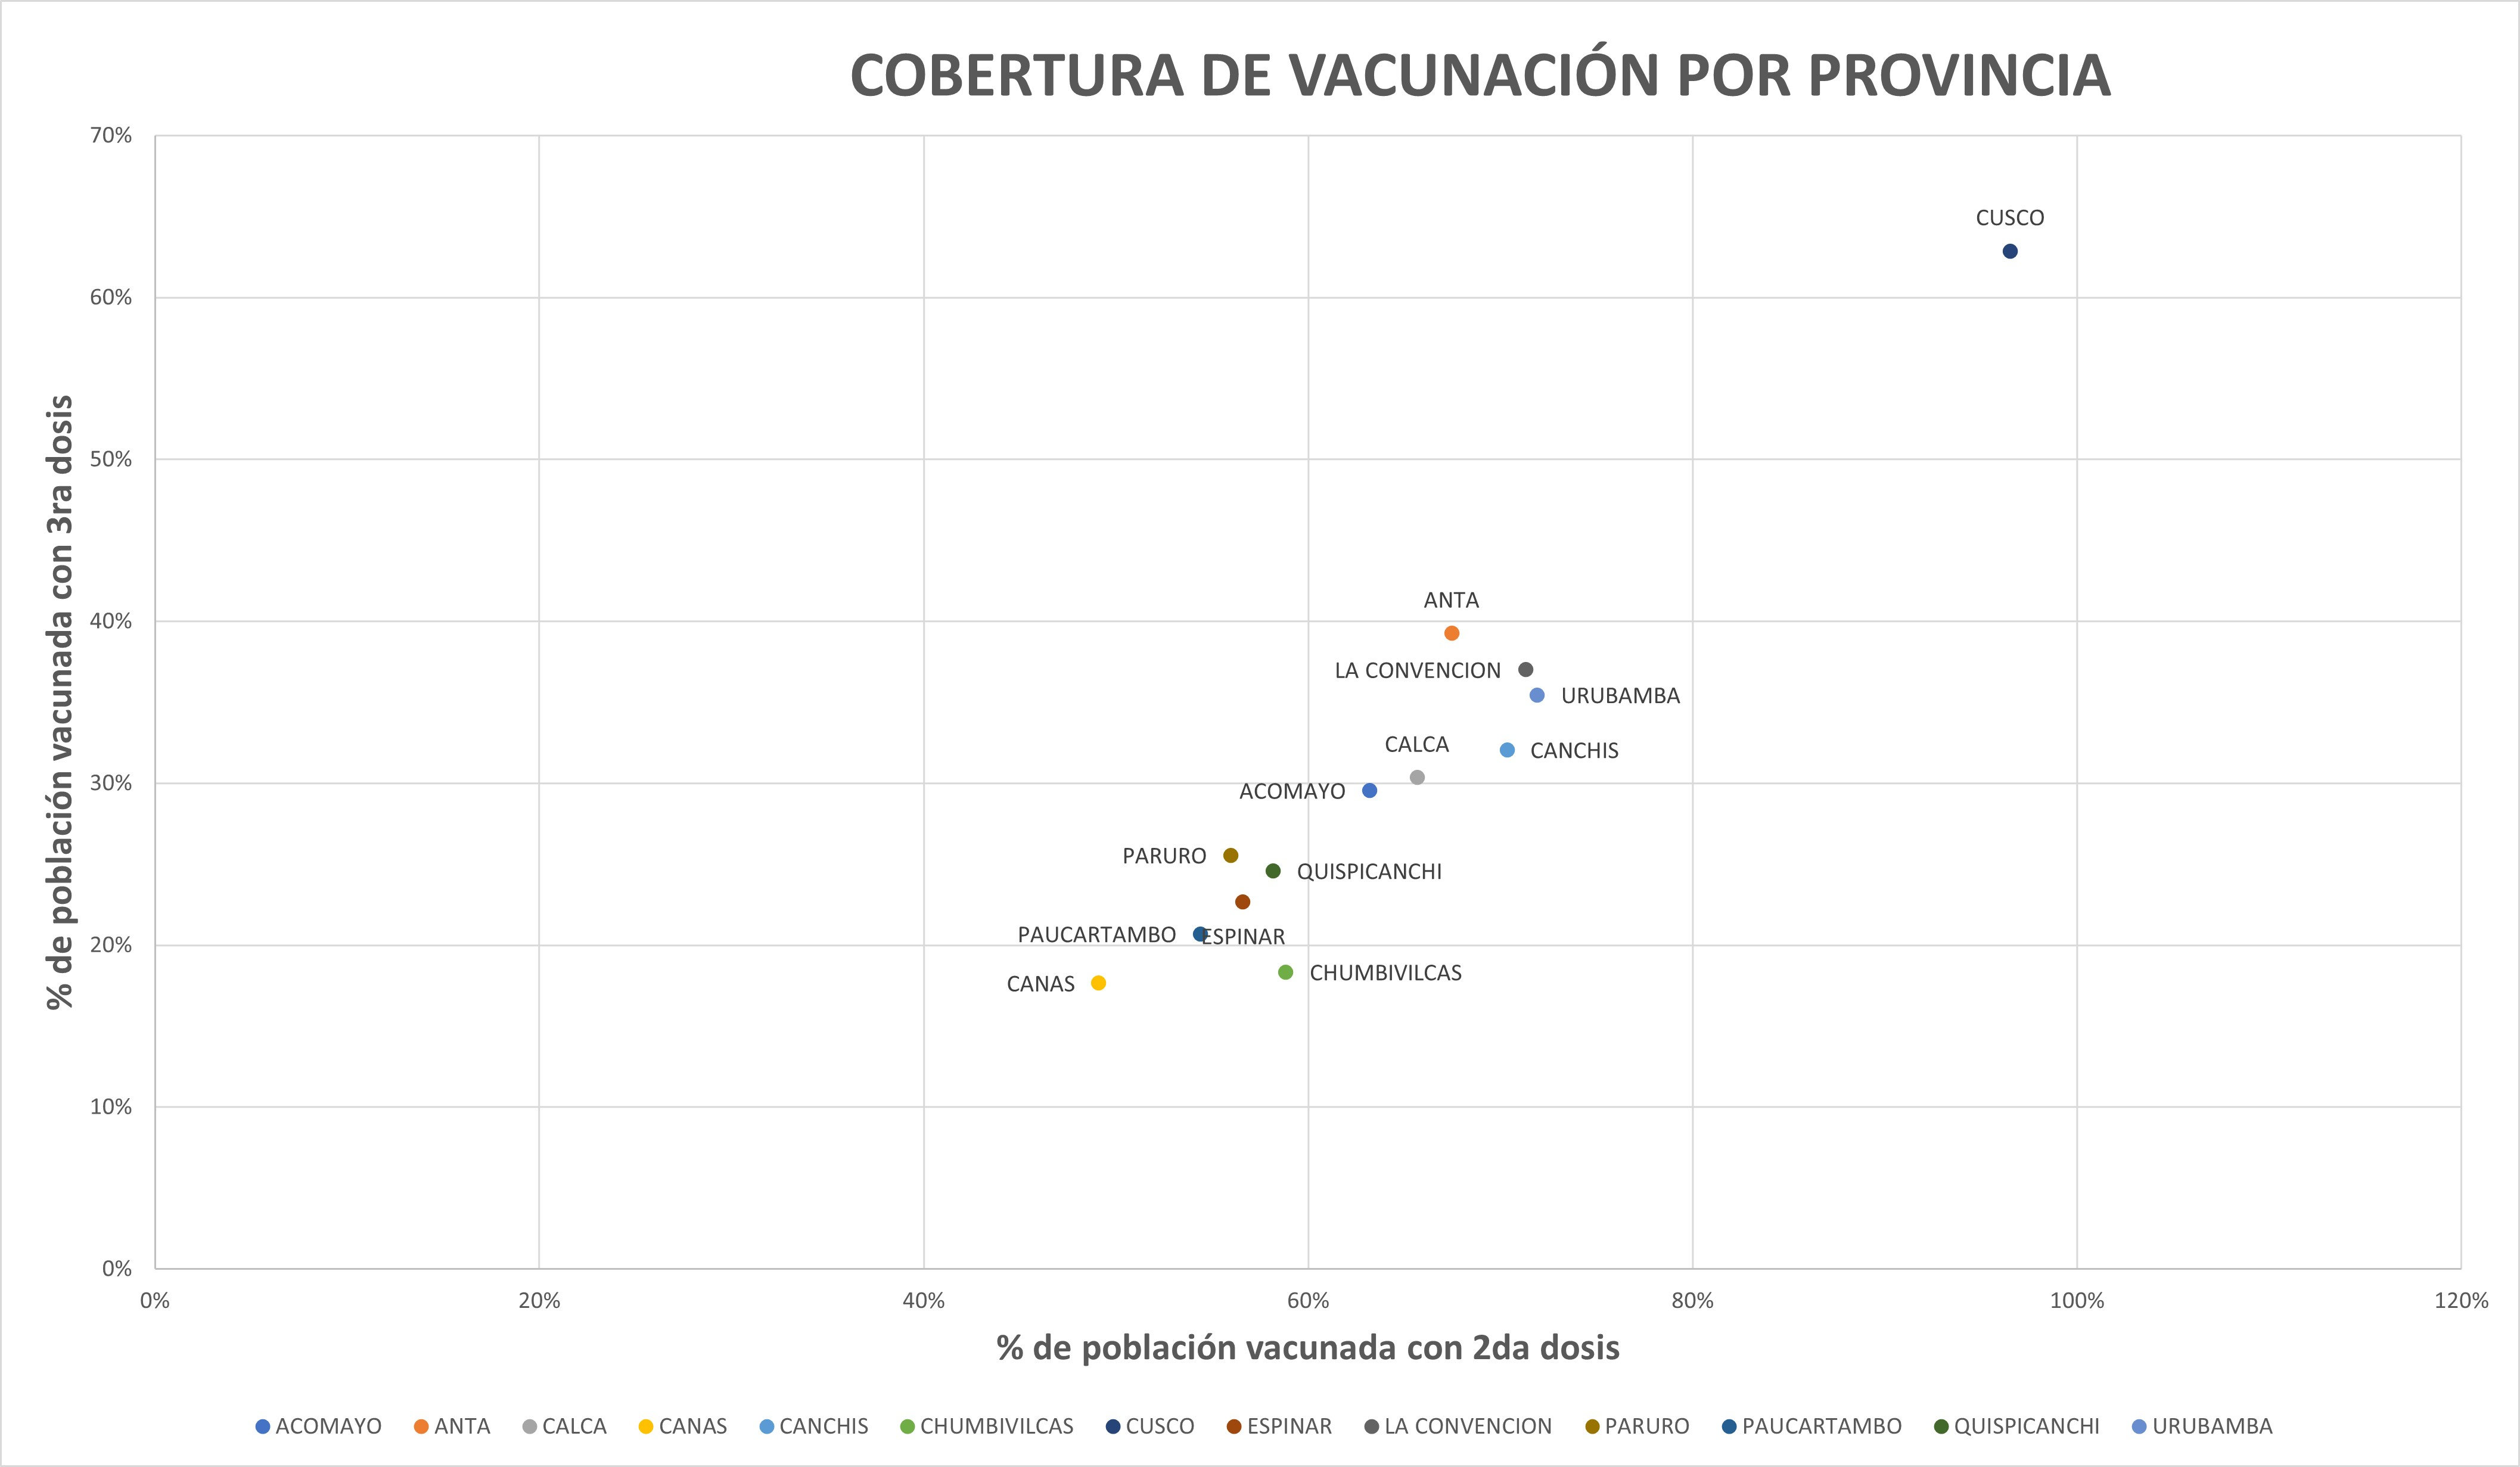
\includegraphics[width=1.0\linewidth, trim={.2cm .2cm .2cm .2cm},clip]{../sala_nacional/Cobertura_Vacunacion_Provincias.jpg}
	\end{center}
	{\tiny Fuente de datos: SICOVAC - HIS MINSA, Dirección de Estadística GERESA Cusco.} 
\end{frame}

\begin{frame}[label=cobertura_vacuna]
	\frametitle{Porcentaje de Cobertura de Vacunación por Grupo de Edad, Región Cusco}
	\vspace{-.5cm}
	\begin{center}
		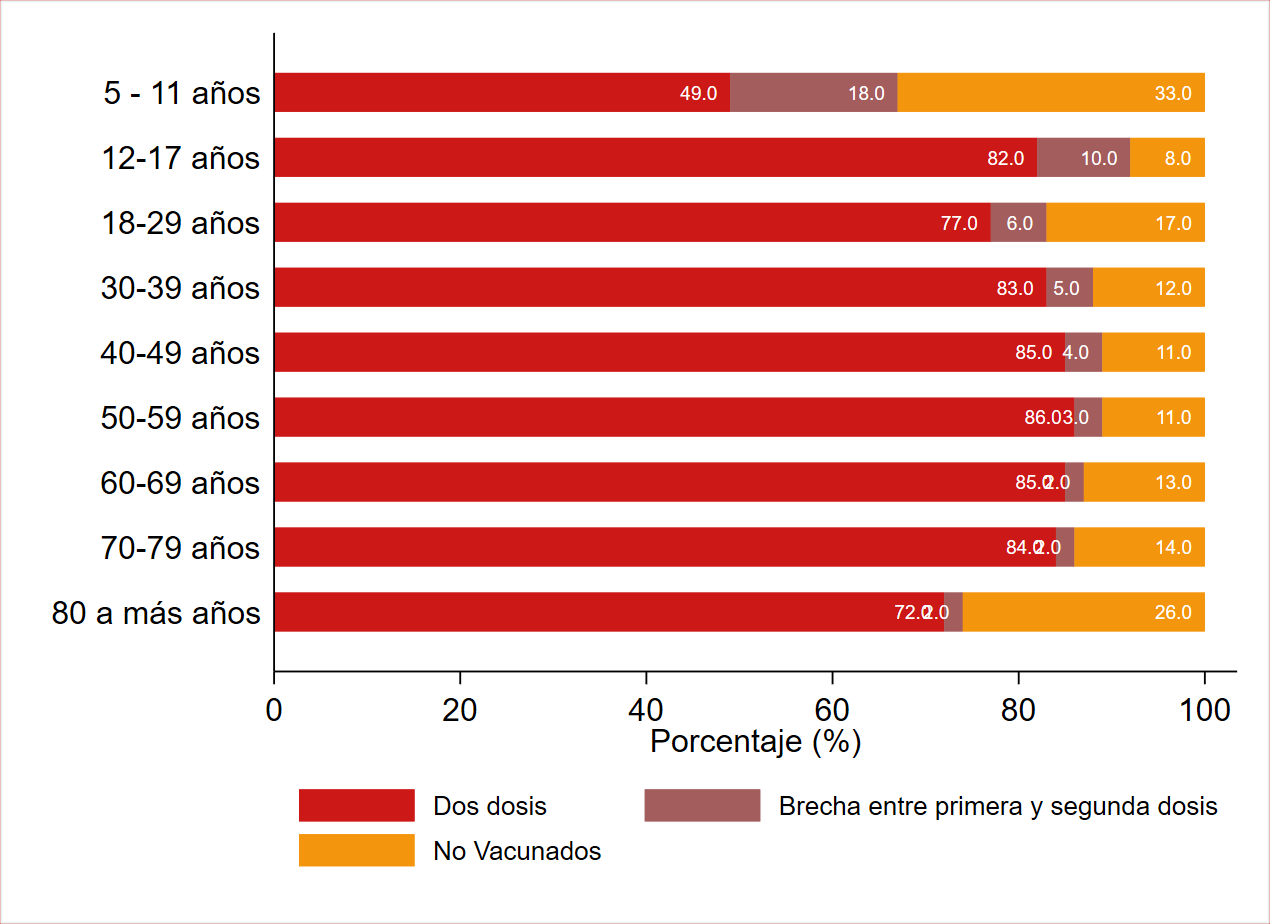
\includegraphics[width=0.8\linewidth, trim={.2cm .5cm .2cm .2cm},clip]{../figuras/vacunacion_grupo_edad.png}
	\end{center}
	{\tiny Fuente de datos: SICOVAC - HIS MINSA, Dirección de Estadística GERESA Cusco.} 
\end{frame}

\begin{frame}[label=cobertura_vacuna_provincias]
	\frametitle{Porcentaje de Cobertura de Vacunación de 80 años a más}
	\vspace{-.5cm}
	\begin{center}
		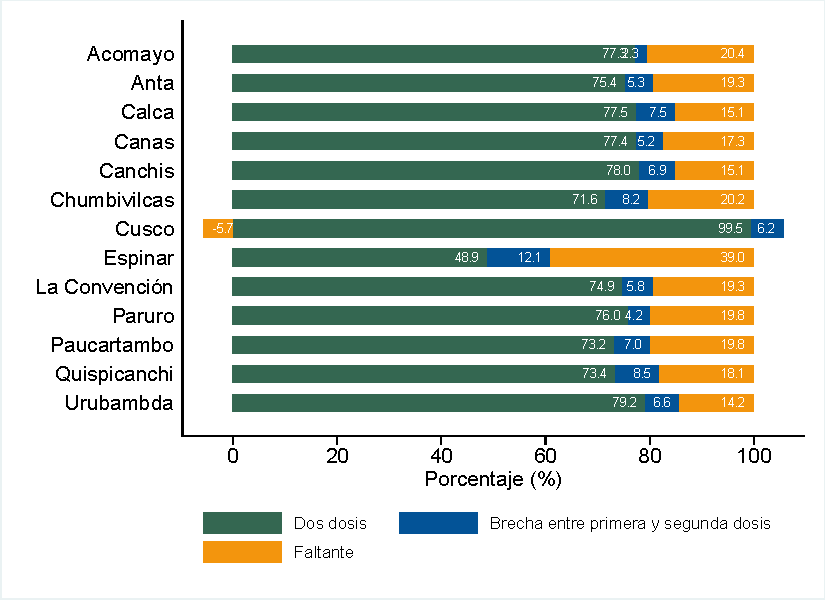
\includegraphics[width=0.8\linewidth, trim={.2cm .5cm .2cm .2cm},clip]{../figuras/vacunacion_provincial_edad_8.pdf}
	\end{center}
	{\tiny Fuente de datos: SICOVAC - HIS MINSA, Dirección de Estadística GERESA Cusco.} \hyperlink{indice}{\beamergotobutton{Índice}}
	
	Ver detalles de estos indicadores para cada grupo de edad de las provincias haciendo clic en los siguientes enlaces:
	\hyperlink{vacunas_70}{\beamergotobutton{60 a 79 años}}
	\hyperlink{vacunas_60}{\beamergotobutton{50 a 59 años}} \hyperlink{vacunas_50}{\beamergotobutton{40 a 49 años}} \hyperlink{vacunas_40}{\beamergotobutton{30 a 39 años}} \hyperlink{vacunas_30}{\beamergotobutton{18 a 29 años}}
	\hyperlink{vacunas_20}{\beamergotobutton{12 a 17 años}} \hyperlink{vacunas_10}{\beamergotobutton{5 a 11 años}}
	
\end{frame}



	%-------------------------------------------------------------------------------------------------------------------------------------------------------------------------------------------------\textit{}-----------------------------------------
	% SECCIÓN 2: Indicadores de Gestión Hospitalaria
	%------------------------------------------------------------------------------------------------------------------------------------------------------------------------------------------------------------------------------------------
	\section{Indicadores de Gestión Hospitalaria}
	
	\begin{frame}[label=camas]
		\frametitle{Total y Ocupación de Camas UCI Hospitalarias, 2021-2022}
		\vspace{-.2cm}
		\begin{center}
			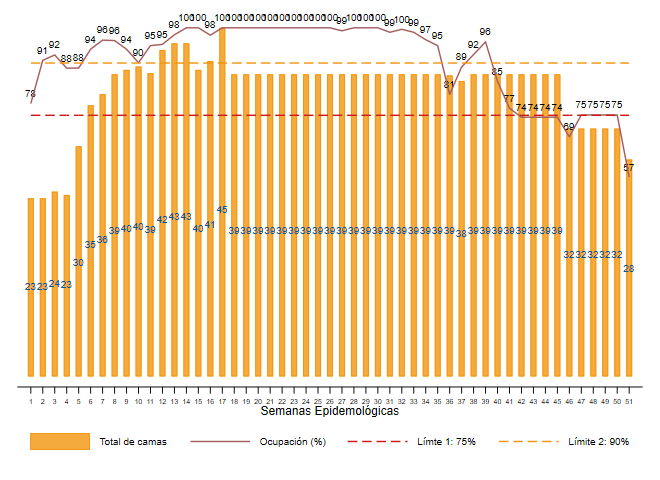
\includegraphics[width=0.9\linewidth, trim={0cm .5cm 0cm 0.2cm},clip]{../figuras/uci.png}		
		\begin{table}[]
			\vspace{-.5cm}
			\resizebox{8 cm}{!}{%
				\begin{tabular}{cccc}
					\hline
					\multicolumn{4}{c}{\textbf{UCIN,   SE 23}}                                                   \\ \hline
					TOTAL CAMAS UCIN & CAMAS   UCIN OCUPADAS & CAMAS   UCIN LIBRES & PORCENTAJE   OCUPACIÓN UCIN \\ \hline
					14               & 04                   & 10                  & 29\%                        \\ \hline
				\end{tabular}%
			}
		\end{table}
		\end{center}
		{\tiny Fuente de datos: Referencias, contrareferencias.}
	\end{frame}
	
	\begin{frame}
		\frametitle{Total y Ocupación de Camas Hospitalarias en el Nivel III, 2021-2022}
		\vspace{-.5cm}
		\begin{center}
			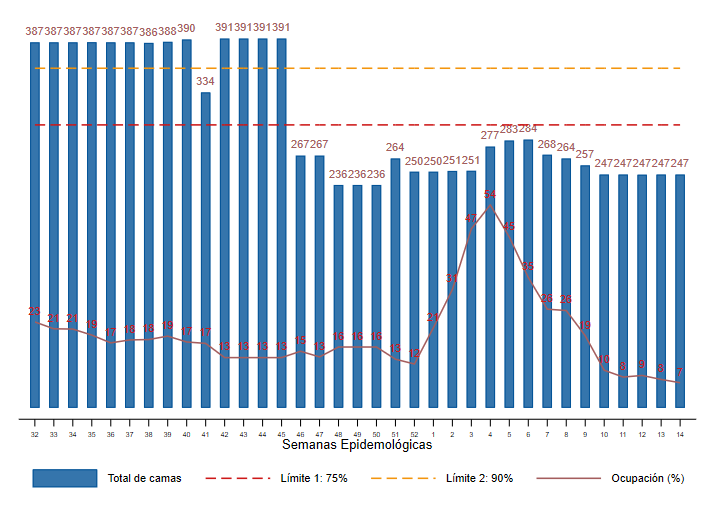
\includegraphics[width=0.8\linewidth, trim={0cm .5cm 0cm 0.2cm},clip]{../figuras/nivel_3.png}
		\end{center}
		{\tiny Fuente de datos: Referencias, contrareferencias.}
	\end{frame}

	\begin{frame}
		\frametitle{Total y Ocupación de Camas Hospitalarias. Hospital Regional, 2021-2022}
		\vspace{-.2cm}
		\begin{center}
			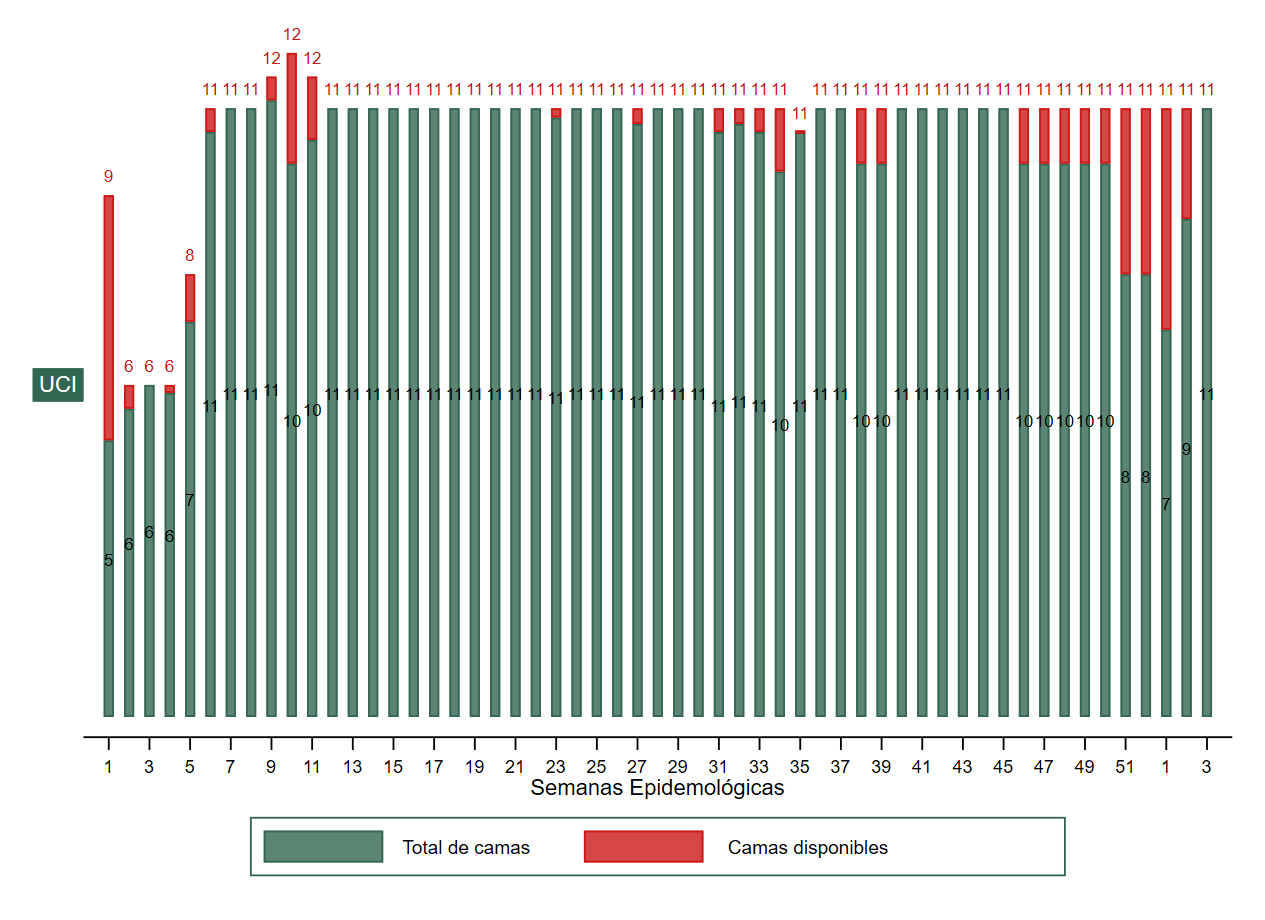
\includegraphics[width=0.9\linewidth, trim={0cm .5cm 0cm 0.2cm},clip]{../figuras/h_regional_uci.png}
		\end{center}
		{\tiny Fuente de datos: Referencias, contrareferencias.}
	\end{frame}
	\begin{frame}
		\frametitle{Total y Ocupación de Camas Hospitalarias. Hospital Regional, 2021-2022}
		\vspace{-.2cm}
		\begin{center}
	-		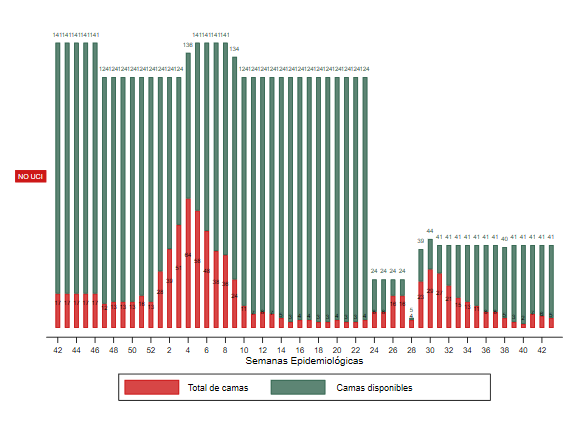
\includegraphics[width=0.8\linewidth, trim={0cm .5cm 0cm 0.2cm},clip]{../figuras/h_regional_nouci.png}
			
			\begin{table}[]
				\resizebox{8 cm}{!}{%
					\begin{tabular}{cccc}
						\hline
						\multicolumn{4}{c}{\textbf{UCIN   HOSPITAL REGIONAL, SE 23}}                                 \\ \hline
						TOTAL CAMAS UCIN & CAMAS   UCIN OCUPADAS & CAMAS   UCIN LIBRES & PORCENTAJE   OCUPACIÓN UCIN \\ \hline
						6               & 3                    & 3                  & 50\%                        \\ \hline
					\end{tabular}%
				}
			\end{table}
			
		\end{center}
		{\tiny Fuente de datos: Referencias, contrareferencias.}
 	\end{frame}
	
	\begin{frame}
		\frametitle{Total y Ocupación de Camas Hospitalarias. Hospital Antonio Lorena, 2021-2022}
		\vspace{-.2cm}
		\begin{center}
			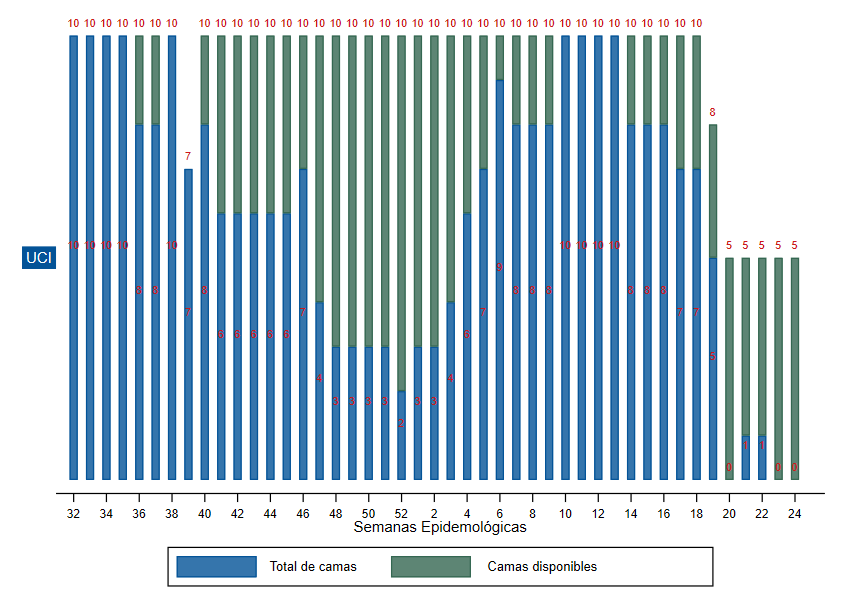
\includegraphics[width=0.77\linewidth, trim={0cm .5cm 0cm 0.2cm},clip]{../figuras/h_lorena_uci.png}				
		\end{center}
		{\tiny Fuente de datos: Referencias, contrareferencias.}
	\end{frame}
	\begin{frame}
		\frametitle{Total y Ocupación de Camas Hospitalarias. Hospital Antonio Lorena, 2021-2022}
		\vspace{-.2cm}
		\begin{center}
			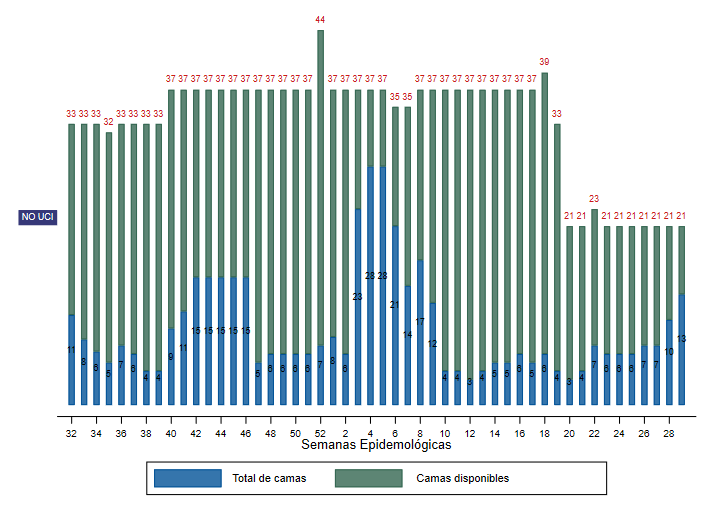
\includegraphics[width=0.8\linewidth, trim={0cm .5cm 0cm 0.2cm},clip]{../figuras/h_lorena_nouci.png}	
			\begin{table}[]
				\resizebox{8 cm}{!}{%
					\begin{tabular}{cccc}
						\hline
						\multicolumn{4}{c}{\textbf{UCIN   HOSPITAL ANTONIO LORENA, SE 23}}                           \\ \hline
						TOTAL CAMAS UCIN & CAMAS   UCIN OCUPADAS & CAMAS   UCIN LIBRES & PORCENTAJE   OCUPACIÓN UCIN \\ \hline
						2                & 1                    & 1                  & 50\%                        \\ \hline
					\end{tabular}%
				}
			\end{table}
			
		\end{center}
		{\tiny Fuente de datos: Referencias, contrareferencias.}
	\end{frame}
	
	\begin{frame}
		\frametitle{Total y Ocupación de Camas Hospitalarias, Hospital Nacional Adolfo Guevara Velasco, 2021-2022}
		\vspace{-.2cm}
		\begin{center}
			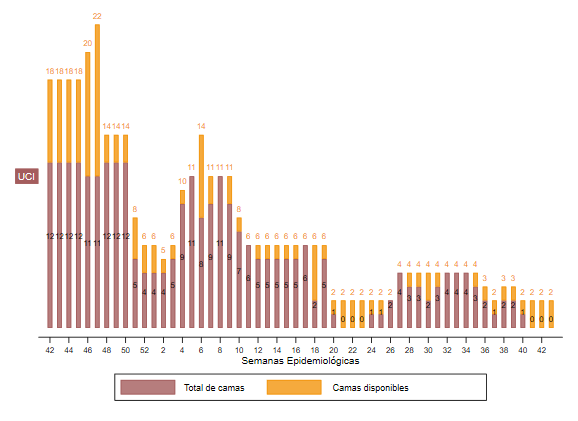
\includegraphics[width=0.77\linewidth, trim={0cm .5cm 0cm 0.2cm},clip]{../figuras/h_adolfo_uci.png}
		\end{center}
		{\tiny Fuente de datos: Referencias, contrareferencias}
	\end{frame}
	\begin{frame}
		\frametitle{Total y Ocupación de Camas Hospitalarias, Hospital Nacional Adolfo Guevara Velasco, 2021-2022}
		\vspace{-.2cm}
		\begin{center}
			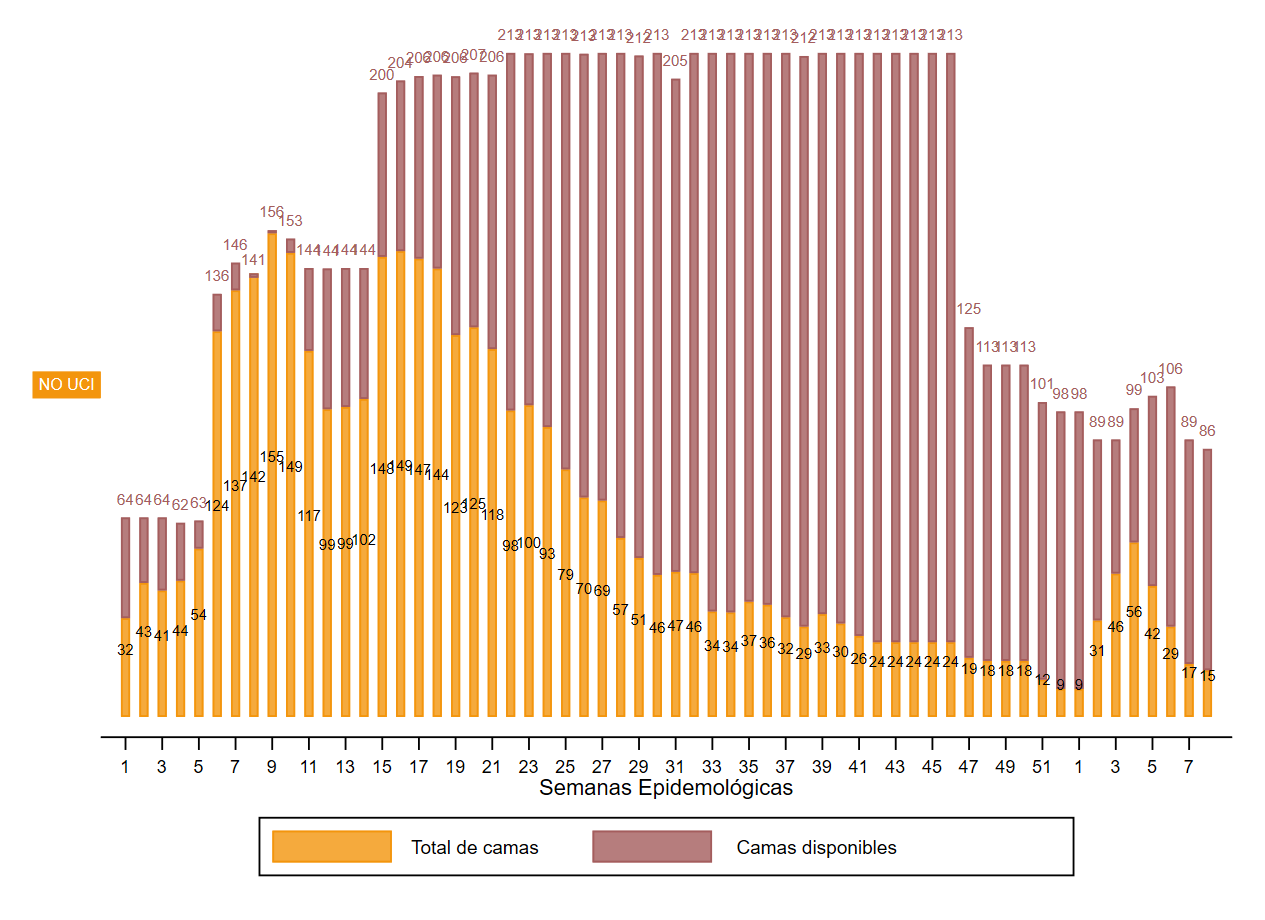
\includegraphics[width=0.8\linewidth, trim={0cm .5cm 0cm 0.2cm},clip]{../figuras/h_adolfo_nouci.png}
			
			\begin{table}[]
				\resizebox{8 cm}{!}{%
					\begin{tabular}{cccc}
						\hline
						\multicolumn{4}{c}{\textbf{UCIN   HOSPITAL ADOLFO GUEVARA, SE 23 }}                           \\ \hline
						TOTAL CAMAS UCIN & CAMAS   UCIN OCUPADAS & CAMAS   UCIN LIBRES & PORCENTAJE   OCUPACIÓN UCIN \\ \hline
						6               & 0                     & 6                   & 0\%                        \\ \hline
					\end{tabular}%
				}
			\end{table}
			
		\end{center}
		{\tiny Fuente de datos: Referencias, contrareferencias}
	\end{frame}
	
	\begin{frame}
		\frametitle{Total y Ocupación de Camas Hospitalarias en el Nivel II, 2021-2022}
		\vspace{-.5cm}
		\begin{center}
			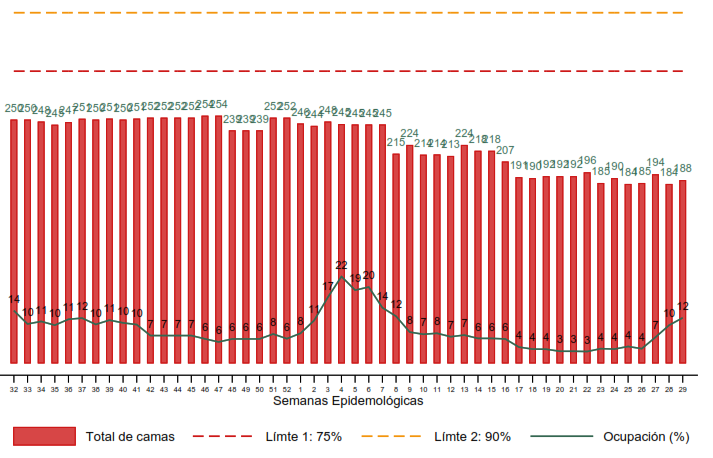
\includegraphics[width=0.8\linewidth, trim={0cm .5cm 0cm 0.2cm},clip]{../figuras/nivel_2.png}
		\end{center}
		{\tiny Fuente de datos: Referencias, contrareferencias.} \hyperlink{indice}{\beamergotobutton{Índice}} 
	\end{frame}
	
	
%-------------------------------------------------------------------------------------------------------------------------------------------------------------------------------------------------\textit{}-----------------------------------------
% SECCIÓN 3: Indicadores por Provincias
%------------------------------------------------------------------------------------------------------------------------------------------------------------------------------------------------------------------------------------------
\section{Indicadores por Provincias}
	\begin{frame}[label=semaforo]
		\frametitle{Tasa de Incidencia por Provincias, 2021-2022}
		\vspace{-.5cm}
		
		% en el input de las tablas sólo debe comenzar y terminar con tabular, borrar el tabular de input de la tabla
		\begin{table}[]
			\resizebox{\textwidth}{!}{%
				\begin{tabular}{lrccclr}
	\rowcolor[HTML]{DCE6F1} 
	\multicolumn{1}{c}{\cellcolor[HTML]{DCE6F1}\textbf{PROVINCIA}} & \multicolumn{1}{c}{\cellcolor[HTML]{DCE6F1}\textbf{Población}} & \textbf{PM+}                                                & \textbf{PA+}         & \textbf{Prueba rápida +} & \multicolumn{1}{c}{\cellcolor[HTML]{DCE6F1}\textbf{Total de casos}} & \multicolumn{1}{c}{\cellcolor[HTML]{DCE6F1}\textbf{Incidencia x 10,000 hab}} \\
	\cellcolor[HTML]{FF5050}CUSCO                                  & 463,656                                                        & 11,072                                                      & 15,872               & 17370                    & 44,314                                                              & 955.75                                                                       \\
	\cellcolor[HTML]{F4B084}LA   CONVENCION                        & 185,793                                                        & 761                                                         & 5,323                & 4915                     & 10,999                                                              & 592.00                                                                       \\
	\cellcolor[HTML]{F4B084}URUBAMBA                               & 66,439                                                         & 152                                                         & 1,610                & 1536                     & 3,298                                                               & 496.40                                                                       \\
	\cellcolor[HTML]{FFE699}CANCHIS                                & 105,049                                                        & 216                                                         & 2,560                & 1731                     & 4,507                                                               & 429.04                                                                       \\
	\cellcolor[HTML]{FFE699}ANTA                                   & 57,731                                                         & 406                                                         & 1,017                & 1012                     & 2,435                                                               & 421.78                                                                       \\
	\cellcolor[HTML]{FFE699}QUISPICANCHI                           & 92,566                                                         & 486                                                         & 1,601                & 1054                     & 3,141                                                               & 339.33                                                                       \\
	\cellcolor[HTML]{FFE699}ESPINAR                                & 71,304                                                         & 15                                                          & 1,020                & 1112                     & 2,147                                                               & 301.11                                                                       \\
	\cellcolor[HTML]{FFE699}CALCA                                  & 76,462                                                         & 118                                                         & 1,143                & 688                      & 1,949                                                               & 254.90                                                                       \\
	\cellcolor[HTML]{FFE699}ACOMAYO                                & 28,477                                                         & 16                                                          & 425                  & 276                      & 717                                                                 & 251.78                                                                       \\
	\cellcolor[HTML]{FFE699}CHUMBIVILCAS                           & 84,925                                                         & 67                                                          & 795                  & 1169                     & 2,031                                                               & 239.15                                                                       \\
	\cellcolor[HTML]{C6E0B4}CANAS                                  & 40,420                                                         & 51                                                          & 526                  & 281                      & 858                                                                 & 212.27                                                                       \\
	\cellcolor[HTML]{C6E0B4}PAUCARTAMBO                            & 52,989                                                         & 109                                                         & 645                  & 253                      & 1,007                                                               & 190.04                                                                       \\
	\cellcolor[HTML]{C6E0B4}PARURO                                 & 31,264                                                         & 56                                                          & 317                  & 211                      & 584                                                                 & 186.80                                                                       \\
	& \multicolumn{1}{l}{}                                           & \multicolumn{1}{l}{}                                        & \multicolumn{1}{l}{} & \multicolumn{1}{l}{}     &                                                                     & \multicolumn{1}{l}{}                                                         \\
	\rowcolor[HTML]{DDEBF7} 
	\textbf{Total   general}                                       & \textbf{1,357,075}                                             & \multicolumn{1}{r}{\cellcolor[HTML]{DDEBF7}\textbf{13,525}} & \textbf{32,854}      & \textbf{31,608}          & \textbf{77,987}                                                     & \textbf{574.67}                                                             
\end{tabular}
			}
		\end{table}
		{\tiny PA: Prueba Antigénica, PM: Prueba Molecular}\\[0.5 cm]
		{\tiny Fuente de datos: SISCOVID, NOTICOVID.}
	\end{frame}
	
	\begin{frame}
		\frametitle{Tasa de Positividad por Provincias, 2021}
		\vspace{-.5cm}
		
		% en el input de las tablas sólo debe comenzar y terminar con tabular, borrar el tabular de input de la tabla
		\begin{table}[]
			\resizebox{\textwidth}{!}{%
				\begin{tabular}{lllll}
	\rowcolor[HTML]{DDEBF7} 
	\multicolumn{1}{c}{\cellcolor[HTML]{DDEBF7}\textbf{PROVINCIA}} & \multicolumn{1}{c}{\cellcolor[HTML]{DDEBF7}\textbf{Total de pruebas}} & \multicolumn{1}{c}{\cellcolor[HTML]{DDEBF7}\textbf{Tasa de positividad general}} & \multicolumn{1}{c}{\cellcolor[HTML]{DDEBF7}\textbf{Tasa de positividad PM}} & \multicolumn{1}{c}{\cellcolor[HTML]{DDEBF7}\textbf{Tasa de positividad Pruebas AG}} \\
	\cellcolor[HTML]{FF5050}URUBAMBA                               & 8,014                                                                 & 19.4                                                                             & 21.2                                                                        & 19.3                                                                                \\
	\cellcolor[HTML]{FF5050}CANAS                                  & 3,509                                                                 & 19.4                                                                             & 12.1                                                                        & 19.6                                                                                \\
	\cellcolor[HTML]{FF5050}CANCHIS                                & 18,035                                                                & 18.8                                                                             & 15.0                                                                        & 19.0                                                                                \\
	\cellcolor[HTML]{FF5050}LA CONVENCIÓN                          & 26,697                                                                & 18.6                                                                             & 22.6                                                                        & 18.4                                                                                \\
	\cellcolor[HTML]{FF5050}CALCA                                  & 5,417                                                                 & 18.1                                                                             & 18.8                                                                        & 18.1                                                                                \\
	\cellcolor[HTML]{FF5050}CUSCO                                  & 166,947                                                               & 17.8                                                                             & 20.4                                                                        & 17.5                                                                                \\
	\cellcolor[HTML]{FF5050}ACOMAYO                                & 2,591                                                                 & 16.6                                                                             & 12.4                                                                        & 17.6                                                                                \\
	\cellcolor[HTML]{FF5050}ANTA                                   & 5,984                                                                 & 16.4                                                                             & 20.4                                                                        & 16.2                                                                                \\
	\cellcolor[HTML]{FF5050}PAUCARTAMBO                            & 4,093                                                                 & 16.4                                                                             & 13.6                                                                        & 16.9                                                                                \\
	\cellcolor[HTML]{FF5050}QUISPICANCHI                           & 10,687                                                                & 15.8                                                                             & 13.1                                                                        & 16.1                                                                                \\
	\cellcolor[HTML]{FF5050}PARURO                                 & 2,700                                                                 & 13.4                                                                             & 17.5                                                                        & 12.5                                                                                \\
	\cellcolor[HTML]{FF5050}CHUMBIVILCAS                           & 11,996                                                                & 11.8                                                                             & 6.4                                                                         & 13.7                                                                                \\
	\cellcolor[HTML]{FF5050}ESPINAR                                & 12,398                                                                & 11.5                                                                             & 15.1                                                                        & 11.4                                                                                \\
	&                                                                       &                                                                                  &                                                                             &                                                                                     \\
	\rowcolor[HTML]{DDEBF7} 
	\textbf{Total   general}                                       & \textbf{279,068}                                                      & \textbf{17.3}                                                                    & \textbf{17.9}                                                               & \textbf{17.2}                                                                      
\end{tabular}
			}
		\end{table}	
		{\tiny Fuente de datos: SISCOVID, NOTICOVID.}
		
	\end{frame}
	
	\begin{frame}
		\frametitle{Defunciones Cero por Provincias por Semana, 2021-2022}
		\vspace{-.5cm}
		
		% en el input de las tablas sólo debe comenzar y terminar con tabular, borrar el tabular de input de la tabla
		\begin{table}[]
			\resizebox{\textwidth}{!}{%
				\begin{tabular}{lccccccccc}
	\textbf{}              	  
	& \multicolumn{1}{l}{}                        
	& \multicolumn{1}{l}{}      
	& \multicolumn{1}{l}{}                         
	& \multicolumn{1}{l}{}                         
	& \multicolumn{1}{l}{}                         
	& \multicolumn{1}{l}{}                        
	& \multicolumn{1}{l}{}                         
	& \multicolumn{1}{l}{} \\                   
	\textbf{}                                                                 				
	&\textbf{SE-31} 							
	&\textbf{SE-32}						
	&\textbf{SE-33}								
	&\textbf{SE-34}					
	&\textbf{SE-35}								
	&\textbf{SE-36}
	&\textbf{SE-37}
	&\textbf{SE-38}\\							
	\textbf{}              	  																
	&\textbf{31jul-06ago}						
	&\textbf{07ago-13ago}						
	&\textbf{14ago-20ago}						
	&\textbf{21ago-27ago}						
	&\textbf{28ago-03sep}
	&\textbf{04sep-10sep}
	&\textbf{11sep-17sep} 
	&\textbf{18sep-24sep} \\
	\textbf{Acomayo}                        												
	&\cellcolor[HTML]{FCC46C}
	&\cellcolor[HTML]{FCC46C}					
	&\cellcolor[HTML]{FCC46C}
	&\cellcolor[HTML]{FCC46C}					
	&\cellcolor[HTML]{FCC46C}
	&\cellcolor[HTML]{FCC46C} 
	&\cellcolor[HTML]{FCC46C}
	&\cellcolor[HTML]{FCC46C}\\
	\textbf{Anta}                                                  				
	&1											
	&\cellcolor[HTML]{FCC46C}					
	&\cellcolor[HTML]{FCC46C}					
	&\cellcolor[HTML]{FCC46C}					
	&\cellcolor[HTML]{FCC46C}
	&\cellcolor[HTML]{FCC46C}	
	&\cellcolor[HTML]{FCC46C}
	&\cellcolor[HTML]{FCC46C}\\					
	\textbf{Calca}      				       									
	&\cellcolor[HTML]{FCC46C}					
	&1											
	&\cellcolor[HTML]{FCC46C}					
	&1											
	&\cellcolor[HTML]{FCC46C}
	&1
	&1
	&\cellcolor[HTML]{FCC46C}\\          			
	\textbf{Canas}                              									
	&\cellcolor[HTML]{FCC46C}
	&1											
	&1
	&\cellcolor[HTML]{FCC46C}					
	&\cellcolor[HTML]{FCC46C}
	&\cellcolor[HTML]{FCC46C}	
	&\cellcolor[HTML]{FCC46C}
	&\cellcolor[HTML]{FCC46C}\\	
	\textbf{Canchis}    						
	&1			
	&\cellcolor[HTML]{FCC46C}					
	&\cellcolor[HTML]{FCC46C}			
	&\cellcolor[HTML]{FCC46C}					
	&1
	&1
	&\cellcolor[HTML]{FCC46C}
	&\cellcolor[HTML]{FCC46C}\\											
	\textbf{Chumbivilcas}                      									
	&\cellcolor[HTML]{FCC46C}
	&\cellcolor[HTML]{FCC46C}					
	&\cellcolor[HTML]{FCC46C}
	&\cellcolor[HTML]{FCC46C}					
	&1
	&\cellcolor[HTML]{FCC46C}
	&1
	&1\\
	\textbf{Cusco}      															
	&2		
	&3											
	&2
	&4											
	&1
	&1
	&\cellcolor[HTML]{FCC46C}
	&\cellcolor[HTML]{FCC46C}\\								
	\textbf{Espinar}       					             							
	&\cellcolor[HTML]{FCC46C}					
	&\cellcolor[HTML]{FCC46C}
	&\cellcolor[HTML]{FCC46C}					
	&\cellcolor[HTML]{FCC46C}
	&\cellcolor[HTML]{FCC46C}					
	&\cellcolor[HTML]{FCC46C}
	&\cellcolor[HTML]{FCC46C}
	&\cellcolor[HTML]{FCC46C}\\	
	\textbf{La Convención}       
	&3											
	&1											
	&2											
	&1											
	&3
	&\cellcolor[HTML]{FCC46C}
	&\cellcolor[HTML]{FCC46C}
	&\cellcolor[HTML]{FCC46C}\\	
	\textbf{Paruro}                            					
	&\cellcolor[HTML]{FCC46C}					
	&\cellcolor[HTML]{FCC46C}					
	&\cellcolor[HTML]{FCC46C}					
	&\cellcolor[HTML]{FCC46C}					
	&\cellcolor[HTML]{FCC46C}
	&\cellcolor[HTML]{FCC46C} 					
	&\cellcolor[HTML]{FCC46C}
	&\cellcolor[HTML]{FCC46C}\\
	\textbf{Paucartambo}               		                       					
	&\cellcolor[HTML]{FCC46C}					
	&\cellcolor[HTML]{FCC46C}
	&\cellcolor[HTML]{FCC46C}					
	&\cellcolor[HTML]{FCC46C}
	&\cellcolor[HTML]{FCC46C}					
	&\cellcolor[HTML]{FCC46C}
	&\cellcolor[HTML]{FCC46C}
	&\cellcolor[HTML]{FCC46C}\\
	\textbf{Quispicanchi}          	      				
	&1											
	&\cellcolor[HTML]{FCC46C}					
	&1											
	&\cellcolor[HTML]{FCC46C}					
	&1
	&\cellcolor[HTML]{FCC46C}
	&\cellcolor[HTML]{FCC46C}
	&\cellcolor[HTML]{FCC46C}\\
	\textbf{Urubamba}  					
	&1											
	&\cellcolor[HTML]{FCC46C}					
	&\cellcolor[HTML]{FCC46C}					
	&1											
	&1	
	&\cellcolor[HTML]{FCC46C}
	&\cellcolor[HTML]{FCC46C}
	&\cellcolor[HTML]{FCC46C}\\						
	&\multicolumn{1}{l}{}                       &\multicolumn{1}{l}{}            &\multicolumn{1}{l}{}                         
	&\multicolumn{1}{l}{}                       &\multicolumn{1}{l}{}            &\multicolumn{1}{l}{}                       &\multicolumn{1}{l}{}                       &\multicolumn{1}{l}{}            			    
\end{tabular}
			}
		\end{table}	
		{\tiny Fuente de datos: SINADEF. \\}
		\vspace{0.5cm}
		$\rightarrow$ Para la SE 23, la provincia del \textbf{\color{mycolor5}Cusco} registro \textbf{\color{mycolor5}cero} defunciones por COVID-19.\\
		$\rightarrow$ Las demás provincias de la región del \textbf{\color{mycolor5}Cusco} registraron \textbf{\color{mycolor5}cero} defunciones por COVID-19.
	\end{frame}
	
	\begin{frame}[label=indicadores_provinciales]
		\frametitle{Tasa de Letalidad y Mortalidad, 2022}
		\vspace{-.5cm}
		
		% en el input de las tablas sólo debe comenzar y terminar con tabular, borrar el tabular de input de la tabla
		\begin{table}[]
			\resizebox{\textwidth}{!}{%
				\begin{tabular}{@{}lrrrrr@{}}
	\rowcolor[HTML]{ECF4FF} 
	\textbf{Provincias}                   & \multicolumn{1}{l}{\cellcolor[HTML]{ECF4FF}\textbf{población}} & \multicolumn{1}{l}{\cellcolor[HTML]{ECF4FF}\textbf{Pruebas Totales}} & \multicolumn{1}{l}{\cellcolor[HTML]{ECF4FF}\textbf{Funciones}} & \multicolumn{1}{l}{\cellcolor[HTML]{ECF4FF}\textbf{Tasa de letalidad}} & \multicolumn{1}{l}{\cellcolor[HTML]{ECF4FF}\textbf{\begin{tabular}[c]{@{}l@{}}tasa de mortalidad x \\   100.000 hab\end{tabular}}} \\
	\cellcolor[HTML]{FD6864}CANCHIS       & 105,049                                                        & 1,545                                                                & 5                                                              & 0.3\%                                                                  & 4.8                                                                                                                                \\
	\cellcolor[HTML]{FD6864}PAUCARTAMBO   & 52,989                                                         & 301                                                                  & 2                                                              & 0.7\%                                                                  & 3.8                                                                                                                                \\
	\cellcolor[HTML]{FD6864}LA CONVENCION & 185,793                                                        & 2,623                                                                & 7                                                              & 0.3\%                                                                  & 3.8                                                                                                                                \\
	\cellcolor[HTML]{FFFC9E}CUSCO         & 463,656                                                        & 16,911                                                               & 9                                                              & 0.1\%                                                                  & 1.9                                                                                                                                \\
	\cellcolor[HTML]{FFFC9E}ESPINAR       & 71,304                                                         & 479                                                                  & 1                                                              & 0.2\%                                                                  & 1.4                                                                                                                                \\
	\cellcolor[HTML]{FFFC9E}CALCA         & 76,462                                                         & 462                                                                  & 1                                                              & 0.2\%                                                                  & 1.3                                                                                                                                \\
	\cellcolor[HTML]{9AFF99}CHUMBIVILCAS  & 84,925                                                         & 448                                                                  & 1                                                              & 0.2\%                                                                  & 1.2                                                                                                                                \\
	\cellcolor[HTML]{9AFF99}QUISPICANCHI  & 92,566                                                         & 735                                                                  & 1                                                              & 0.1\%                                                                  & 1.1                                                                                                                                \\
	\cellcolor[HTML]{9AFF99}ACOMAYO       & 28,477                                                         & 149                                                                  & 0                                                              & 0.0\%                                                                  & 0.0                                                                                                                                \\
	\cellcolor[HTML]{9AFF99}ANTA          & 57,731                                                         & 480                                                                  & 0                                                              & 0.0\%                                                                  & 0.0                                                                                                                                \\
	\cellcolor[HTML]{9AFF99}CANÁS         & 40,420                                                         & 206                                                                  & 0                                                              & 0.0\%                                                                  & 0.0                                                                                                                                \\
	\cellcolor[HTML]{9AFF99}PARURO        & 31,264                                                         & 132                                                                  & 0                                                              & 0.0\%                                                                  & 0.0                                                                                                                                \\
	\cellcolor[HTML]{9AFF99}URUBAMBÁ      & 66,439                                                         & 900                                                                  & 0                                                              & 0.0\%                                                                  & 0.0                                                                                                                                \\
	& \multicolumn{1}{l}{}                                           & \multicolumn{1}{l}{}                                                 & \multicolumn{1}{l}{}                                           & \multicolumn{1}{l}{}                                                   & \multicolumn{1}{l}{}                                                                                                               \\
	\rowcolor[HTML]{ECF4FF} 
	\textbf{Totales generales}            & \textbf{1,357,075}                                             & \textbf{25,371}                                                      & \textbf{27}                                                    & \textbf{0.11\%}                                                        & \textbf{2.0}                                                                                                                      
\end{tabular}
			}
		\end{table}
		{\tiny Fuente de datos: SINADEF. \hyperlink{indice}{\beamergotobutton{Índice}} \\} 
		
		Ver detalles de la tendencia (2020 y 2021-2022) de estos indicadores para cada provincia haciendo clic en los siguientes enlaces:\\ \hyperlink{Acomayo}{\beamergotobutton{Acomayo}} \hyperlink{Anta}{\beamergotobutton{Anta}} \hyperlink{Calca}{\beamergotobutton{Calca}} \hyperlink{Canas}{\beamergotobutton{Canas}} \hyperlink{Chumbivilcas}{\beamergotobutton{Chimbivilcas}}
		\hyperlink{Canchis}{\beamergotobutton{Canchis}} \hyperlink{Cusco}{\beamergotobutton{Cusco}}
		\hyperlink{Espinar}{\beamergotobutton{Espinar}}
		\hyperlink{laconvencion}{\beamergotobutton{La Convencion}}
		\hyperlink{Paruro}{\beamergotobutton{Paruro}} \hyperlink{Paucartambo}{\beamergotobutton{Paucartambo}}	
		\hyperlink{Quispicanchi}{\beamergotobutton{Quispicanchi}}
		\hyperlink{Urubamba}{\beamergotobutton{Urubamba}}
	\end{frame}

%-------------------------------------------------------------------------------------------------------------------------------------------------------------------------------------------------\textit{}-----------------------------------------
% SECCIÓN 4: Resúmen y Recomendaciones
%------------------------------------------------------------------------------------------------------------------------------------------------------------------------------------------------------------------------------------------
\section{Resumen}
\begin{frame}[label=Resumen]
	\frametitle{Análisis Situacional por COVID-19: Resumen}
	\vspace{-.5cm}
	\begin{itemize}
		\item La Región de Cusco se ubica en el \textbf{\color{mycolor4}octavo lugar} de \textbf{\color{mycolor3}mortalidad} acumulada a nivel nacional, con un índice de propagación de $0.8 $.   
		\item Existe un \textbf{\color{mycolor4} incremento} en el número de \textbf{\color{mycolor3}casos}, siendo estos últimos a predominio de casos asintomáticos para la SE 23. 
		\item La \textbf{\color{mycolor3}tasa de positividad para pruebas moleculares}  se encuentra \textbf{\color{mycolor4}en ascenso} con un $7.7\%$, así como la \textbf{\color{mycolor3}tasa de positividad de pruebas antigénicas}  presenta un ligero ascenso a $3.2\%$.
	\end{itemize}
\end{frame}

\begin{frame}
	\frametitle{Análisis Situacional por COVID-19: Resumen}
	\vspace{-.5cm}
	\begin{itemize}
	\item La ocupación de camas \textbf{\color{mycolor3}UCI} \textbf{\color{mycolor4}disminuyó} al $20\%$ a nivel regional.
	\item La ocupación de camas \textbf{\color{mycolor3}no UCI}, \textbf{\color{mycolor4}se mantuvo estable} con el $7\%$.
	\item Para la SE 23, predomina la variante ómicron en el $98\%$, del total de muestras secuenciadas por semana, siendo las características de presentación clínica similares con las otras variantes, con casos leves en la presentación clínica, secuenciamiento que se realiza en nuestra región desde hace 02 semanas.
	\item La \textbf{\color{mycolor3}cobertura de vacunación regional} para COVID-19, muestra una \textbf{\color{mycolor4}cobertura por encima del $80\%$ para los grupos etarios mayores a 50 años}, con una brecha más amplia en los grupos etarios menores a 39 años.
	
	\end{itemize}
\end{frame}

\begin{frame}
	\frametitle{Análisis Situacional por COVID-19: Resumen}
	\vspace{-.5cm}
	\begin{itemize}
		\item Semáforo epidemiológico regional
		\begin{itemize}
			\item Tasa de crecimiento semanal de \textbf{\color{mycolor4}casos} en \textbf{\color{mycolor3}verde}.
			\item Tasa de crecimiento semanal de \textbf{\color{mycolor4}defunciones} en \textbf{\color{mycolor3}verde}.
			\item Tasa de \textbf{\color{mycolor4}positividad} de pruebas \textbf{\color{mycolor4}antigénicas} en \textbf{\color{mycolor3}verde}, mientras que la pruebas \textbf{\color{mycolor4}moleculares} cambió a \textbf{\color{mycolor3}ámbar}
			\item Disponibilidad de \textbf{\color{mycolor4}camas hospitalarias}: no UCI: en \textbf{\color{mycolor3}verde}.
			\item Disponibilidad de camas hospitalarias: \textbf{\color{mycolor4}UCI} en \textbf{\color{mycolor3}verde}.
		\end{itemize} 
		\item Semáforo epidemiológico a nivel provincial
		\begin{itemize}
			\item Para la SE23, se presenta un ascenso en el número de casos, aún se mantienen bajas las defunciones y hospitalizaciones.
		\end{itemize}
	\end{itemize}
\end{frame}

\begin{frame}[label=recomendaciones]
	\frametitle{Análisis Situacional por COVID-19: Recomendaciones}
	\vspace{-.5cm}
	\begin{itemize}
			\item Reforzar medidas de control por comandos C19 provinciales y distritales, con medidas de fiscalización
			\item Mejorar las brechas de vacunación, con énfasis en la 3ra dosis.
			\item Énfasis en distanciamiento social, mascarilla y ambientes ventilados
			\item Campañas de comunicación (mensajes claros, consistentes y constantes)
			\item Aislamiento temprano de casos y contactos
			\item Conservar la burbuja familiar. 
			\item Fortalecer la búsqueda activa de casos y contactos
			\item Fortalecer el seguimiento clínico de casos			
	\end{itemize} 
\end{frame}

\section{Links Útiles\footnote{Agradecimiento: Diseño: Johar Cassa y Jason Cruz}}

\begin{frame}[label=links]
	\frametitle{Links Útiles}
	\vspace{-.5cm}
	\begin{itemize}
		\item Encuentre {\color{mycolor4} información de la pandemia actualizada diaria a nivel regional, provincial, y distrital} en nuestro {\color{mycolor4}\textbf{Dashboard GERESA}} haciendo clic \href{https://geresacusc.shinyapps.io/GERESA_dashboard/}{\color{mycolor2}aquí}.
		\item Encuentre información actualizada de los {\color{mycolor4}Mapas de Calor COVID-19} en el haciendo clic \href{http://www.diresacusco.gob.pe/diresa/}{\color{mycolor2}aquí}.
		\item Encuentre información diaria del {\color{mycolor4} Resumen de la Sala Situacional COVID-19} de la Región haciendo clic \href{https://app.powerbi.com/view?r=eyJrIjoiZDdiMzA4YWMtZTZmNC00ZWE2LWFmMmYtODkwZmM1ODhiYTljIiwidCI6IjM2NGE0NmEwLTk0YzctNGZkNi1iYTNjLTlmMmQzMjA5YzFlZiJ9}{\color{mycolor2}aquí}.
		\item Encuentre información resumen cuatro semanas de la situación epidemiológica de COVID-19 en los {\color{mycolor4}Boletines COVID-19} haciendo clic \href{https://sites.google.com/view/geresacusco/boletines-epidemiologicos-covid-19}{\color{mycolor2}aquí}. \hyperlink{indice}{\beamergotobutton{Índice}}
	\end{itemize}
\end{frame}


%------------------------------------------------------------------------------------------------------------------------------------------------------------------------------------------------------------------------------------------
% APÉNDICE
%------------------------------------------------------------------------------------------------------------------------------------------------------------------------------------------------------------------------------------------

%\backupbegin

%\setbeamercovered{invisible}
%\begin{frame}[plain,noframenumbering]
%	\titlepage
%\end{frame}

\appendix
\section{Apéndice}

\subsection{Vacunación por Provincias y Grupo de Edad}

\begin{frame}[label=vacunas_70]
	\frametitle{Porcentaje de Cobertura de Vacunación de 60 a 79 años}
	\vspace{-.5cm}
	\begin{center}
		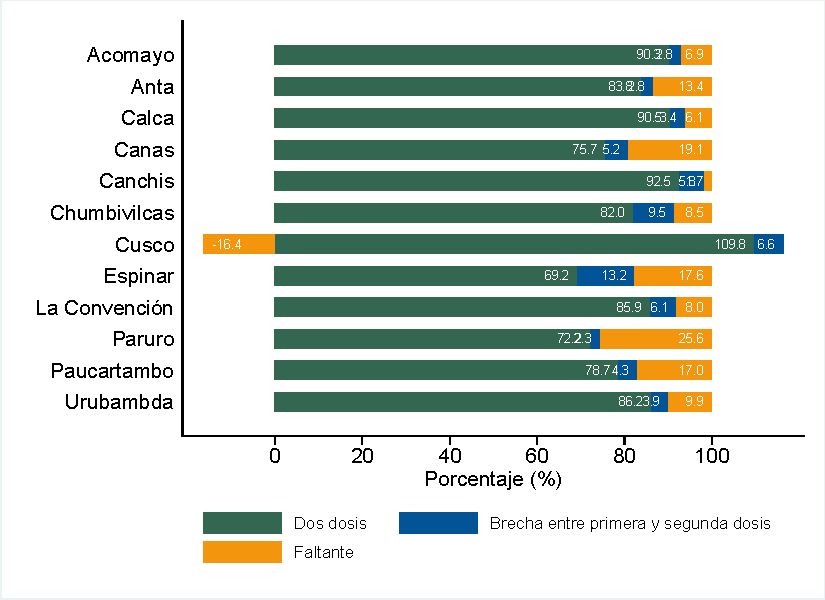
\includegraphics[width=0.8\linewidth, trim={.2cm .5cm .2cm .2cm},clip]{../figuras/vacunacion_provincial_edad_7.pdf}
	\end{center}
	{\tiny Fuente de datos: SICOVAC - HIS MINSA, Dirección de Estadística GERESA Cusco. \\}
\hyperlink{cobertura_vacuna_provincias}{\beamergotobutton{regresar}}
\end{frame}

\begin{frame}[label=vacunas_60]
	\frametitle{Porcentaje de Cobertura de Vacunación de 50 a 59 años, Provincias de Cusco}
	\vspace{-.5cm}
	\begin{center}
		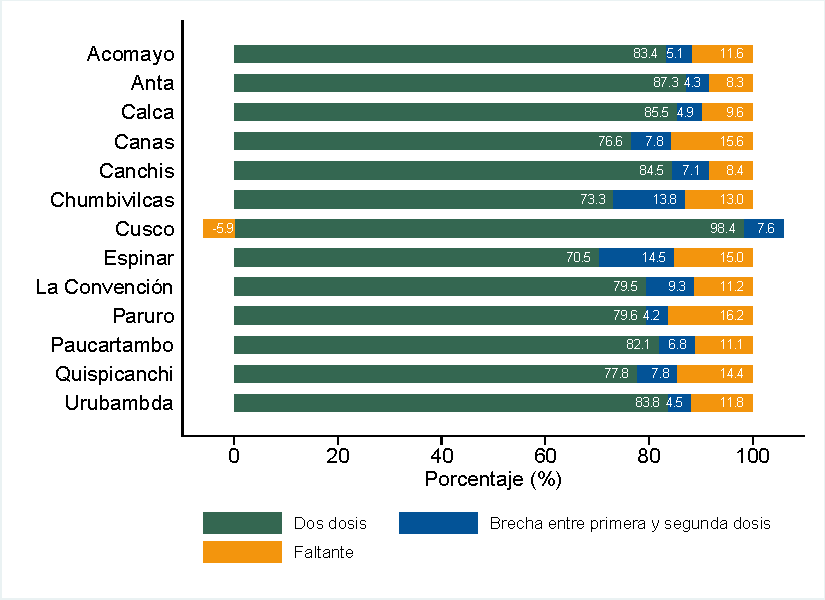
\includegraphics[width=0.8\linewidth, trim={.2cm .5cm .2cm .2cm},clip]{../figuras/vacunacion_provincial_edad_6.pdf}
	\end{center}
	{\tiny Fuente de datos: SICOVAC - HIS MINSA, Dirección de Estadística GERESA Cusco. \\}
	\hyperlink{cobertura_vacuna_provincias}{\beamergotobutton{regresar}}
\end{frame}

\begin{frame}[label=vacunas_50]
	\frametitle{Porcentaje de Cobertura de Vacunación de 40 a 49 años, Provincias de Cusco}
	\vspace{-.5cm}
	\begin{center}
		\includegraphics[width=0.8\linewidth, trim={.2cm .5cm .2cm .2cm},clip]{../figuras/vacunacion_provincial_edad_5.pdf}
	\end{center}
	{\tiny Fuente de datos: SICOVAC - HIS MINSA, Dirección de Estadística GERESA Cusco. \\}
\hyperlink{cobertura_vacuna_provincias}{\beamergotobutton{regresar}}
\end{frame}

\begin{frame}[label=vacunas_40]
	\frametitle{Porcentaje de Cobertura de Vacunación de 30 a 39 años, Provincias de Cusco}
	\vspace{-.5cm}
	\begin{center}
		\includegraphics[width=0.8\linewidth, trim={.2cm .5cm .2cm .2cm},clip]{../figuras/vacunacion_provincial_edad_4.pdf}
	\end{center}
	{\tiny Fuente de datos: SICOVAC - HIS MINSA, Dirección de Estadística GERESA Cusco. \\}
\hyperlink{cobertura_vacuna_provincias}{\beamergotobutton{regresar}}
\end{frame}

\begin{frame}[label=vacunas_30]
	\frametitle{Porcentaje de Cobertura de Vacunación de 18 a 29 años, Provincias de Cusco}
	\vspace{-.5cm}
	\begin{center}
		\includegraphics[width=0.8\linewidth, trim={.2cm .5cm .2cm .2cm},clip]{../figuras/vacunacion_provincial_edad_3.pdf}
	\end{center}
	{\tiny Fuente de datos: SICOVAC - HIS MINSA, Dirección de Estadística GERESA Cusco. \\}
\hyperlink{cobertura_vacuna_provincias}{\beamergotobutton{regresar}}
\end{frame}

\begin{frame}[label=vacunas_20]
	\frametitle{Porcentaje de Cobertura de Vacunación de 12 a 17 años, Provincias de Cusco}
	\vspace{-.5cm}
	\begin{center}
		\includegraphics[width=0.8\linewidth, trim={.2cm .5cm .2cm .2cm},clip]{../figuras/vacunacion_provincial_edad_2.pdf}
	\end{center}
	{\tiny Fuente de datos: SICOVAC - HIS MINSA, Dirección de Estadística GERESA Cusco. \\}
\hyperlink{cobertura_vacuna_provincias}{\beamergotobutton{regresar}}

\end{frame}

\begin{frame}[label=vacunas_10]
	\frametitle{Porcentaje de Cobertura de Vacunación de 05 a 11 años, Provincias de Cusco}
	\vspace{-.5cm}
	\begin{center}
		\includegraphics[width=0.8\linewidth, trim={.2cm .5cm .2cm .2cm},clip]{../figuras/vacunacion_provincial_edad_1.pdf}
	\end{center}
	{\tiny Fuente de datos: SICOVAC - HIS MINSA, Dirección de Estadística GERESA Cusco. \\}
\hyperlink{cobertura_vacuna_provincias}{\beamergotobutton{regresar}}
\end{frame}

\subsection{Acomayo}
\begin{frame}[label=Acomayo]
	\frametitle{Curva Epidemica de Sintomaticos por Tipo de Prueba, Provincia Acomayo}
	\vspace{-.5cm}
	\begin{center}
		\includegraphics[width=0.8\linewidth, trim={0cm .5cm 0cm 0.2cm},clip]{../figuras/sinto_prueba20_21_1.png}
	\end{center}
	{\tiny Fuente de datos: SISCOVID, NOTICOVID, SINADEF.}
	\hyperlink{TipoPrueba}{\beamergotobutton{regresar}}
\end{frame}

\begin{frame}[label=Acomayo]
	\frametitle{Incidencia y Mortalidad, Provincia Acomayo}
	\vspace{-.5cm}
	\begin{center}
		\includegraphics[width=0.8\linewidth, trim={0cm .5cm 0cm 0.2cm},clip]{../figuras/incidencia_mortalidad_20_21_1.png}
	\end{center}
	{\tiny Fuente de datos: SISCOVID, NOTICOVID, SINADEF.}
\end{frame}

\begin{frame}
	\frametitle{Tasa de Positividad, Provincia Acomayo}
	\vspace{-.5cm}
	\begin{center}
		\includegraphics[width=0.8\linewidth, trim={0cm .5cm 0cm 0.2cm},clip]{../figuras/positividad_20_21_1.png}
	\end{center}
	{\tiny Fuente de datos: SISCOVID, NOTICOVID.}
\end{frame}

\begin{frame}
	\frametitle{Exceso de Defunciones por Todas las Causas, Provincia Acomayo}
	\vspace{-.5cm}
	\begin{center}	
		\includegraphics[width=0.8\linewidth, trim={0cm .5cm 0cm 0.2cm},clip]{../figuras/exceso_1.pdf}
	\end{center}
	{\tiny Fuente de datos: SINADEF.}
	
	\hyperlink{indicadores_provinciales}{\beamergotobutton{regresar}}
\end{frame}

\subsection{Anta}
\begin{frame}[label=Anta]
	\frametitle{Curva Epidemica de Sintomaticos por Tipo de Prueba, Provincia Anta}
	\vspace{-.5cm}
	\begin{center}
		\includegraphics[width=0.8\linewidth, trim={0cm .5cm 0cm 0.2cm},clip]{../figuras/sinto_prueba20_21_2.png}
	\end{center}
	{\tiny Fuente de datos: SISCOVID, NOTICOVID, SINADEF.}
	\hyperlink{TipoPrueba}{\beamergotobutton{regresar}}
\end{frame}

\begin{frame}[label=Anta]
	\frametitle{Incidencia y Mortalidad, Provincia Anta}
	\vspace{-.5cm}
	\begin{center}
		\includegraphics[width=0.8\linewidth, trim={0cm .5cm 0cm 0.2cm},clip]{../figuras/incidencia_mortalidad_20_21_2.png}
	\end{center}
	{\tiny Fuente de datos: SISCOVID, NOTICOVID, SINADEF.}
\end{frame}

\begin{frame}
	\frametitle{Tasa de Positividad, Provincia Anta}
	\vspace{-.5cm}
	\begin{center}
		\includegraphics[width=0.8\linewidth, trim={0cm .5cm 0cm 0.2cm},clip]{../figuras/positividad_20_21_2.png}
	\end{center}
	{\tiny Fuente de datos: SISCOVID, NOTICOVID.}
\end{frame}

\begin{frame}
	\frametitle{Exceso de Defunciones por Todas las Causas, Provincia Anta}
	\vspace{-.5cm}
	\begin{center}
		\includegraphics[width=0.8\linewidth, trim={0cm .5cm 0cm 0.2cm},clip]{../figuras/exceso_2.pdf}
	\end{center}
	{\tiny Fuente de datos: SINADEF.}
	
	\hyperlink{indicadores_provinciales}{\beamergotobutton{regresar}}
\end{frame}

\subsection{Calca}
\begin{frame}[label=Calca]
	\frametitle{Curva Epidemica de Sintomaticos por Tipo de Prueba, Provincia Calca}
	\vspace{-.5cm}
	\begin{center}
		\includegraphics[width=0.8\linewidth, trim={0cm .5cm 0cm 0.2cm},clip]{../figuras/sinto_prueba20_21_3.png}
	\end{center}
	{\tiny Fuente de datos: SISCOVID, NOTICOVID, SINADEF.}
	\hyperlink{TipoPrueba}{\beamergotobutton{regresar}}
\end{frame}

\begin{frame}[label=Calca]
	\frametitle{Incidencia y Mortalidad, Provincia Calca}
	\vspace{-.5cm}
	\begin{center}
		\includegraphics[width=0.8\linewidth, trim={0cm .5cm 0cm 0.2cm},clip]{../figuras/incidencia_mortalidad_20_21_3.png}
	\end{center}
	{\tiny Fuente de datos: SISCOVID, NOTICOVID, SINADEF.}
\end{frame}

\begin{frame}
	\frametitle{Tasa de Positividad, Provincia Calca}
	\vspace{-.5cm}
	\begin{center}
		\includegraphics[width=0.8\linewidth, trim={0cm .5cm 0cm 0.2cm},clip]{../figuras/positividad_20_21_3.png}
	\end{center}
	{\tiny Fuente de datos: SISCOVID, NOTICOVID.}
\end{frame}

\begin{frame}
	\frametitle{Exceso de Defunciones por Todas las Causas, provincia Calca}
	\vspace{-.5cm}
	\begin{center}
		\includegraphics[width=0.8\linewidth, trim={0cm .5cm 0cm 0.2cm},clip]{../figuras/exceso_3.pdf}
	\end{center}
	{\tiny Fuente de datos: SINADEF.}
	
	\hyperlink{indicadores_provinciales}{\beamergotobutton{regresar}}
\end{frame}

\subsection{Canas}
\begin{frame}[label=Canas]
	\frametitle{Curva Epidemica de Sintomaticos por Tipo de Prueba, Provincia Canas}
	\vspace{-.5cm}
	\begin{center}
		\includegraphics[width=0.8\linewidth, trim={0cm .5cm 0cm 0.2cm},clip]{../figuras/sinto_prueba20_21_4.png}
	\end{center}
	{\tiny Fuente de datos: SISCOVID, NOTICOVID, SINADEF.}
	\hyperlink{TipoPrueba}{\beamergotobutton{regresar}}
\end{frame}

\begin{frame}[label=Canas]
	\frametitle{Incidencia y Mortalidad, Provincia Canas}
	\vspace{-.5cm}
	\begin{center}
		\includegraphics[width=0.8\linewidth, trim={0cm .5cm 0cm 0.2cm},clip]{../figuras/incidencia_mortalidad_20_21_4.png}
	\end{center}
	{\tiny Fuente de datos: SISCOVID, NOTICOVID, SINADEF}
\end{frame}

\begin{frame}
	\frametitle{Tasa de positividad, Provincia Canas}
	\vspace{-.5cm}
	\begin{center}
		\includegraphics[width=0.8\linewidth, trim={0cm .5cm 0cm 0.2cm},clip]{../figuras/positividad_20_21_4.png}
	\end{center}
	{\tiny Fuente de datos: SISCOVID, NOTICOVID.}
\end{frame}

\begin{frame}
	\frametitle{Exceso de Defunciones por Todas las Causas, provincia Canas}
	\vspace{-.5cm}
	\begin{center}
		\includegraphics[width=0.8\linewidth, trim={0cm .5cm 0cm 0.2cm},clip]{../figuras/exceso_4.pdf}
	\end{center}
	{\tiny Fuente de datos: SINADEF.}
	
	\hyperlink{indicadores_provinciales}{\beamergotobutton{regresar}}
\end{frame}

\subsection{Canchis}
\begin{frame}[label=Canchis]
	\frametitle{Curva Epidemica de Sintomaticos por Tipo de Prueba, Provincia Canchis}
	\vspace{-.5cm}
	\begin{center}
		\includegraphics[width=0.8\linewidth, trim={0cm .5cm 0cm 0.2cm},clip]{../figuras/sinto_prueba20_21_5.png}
	\end{center}
	{\tiny Fuente de datos: SISCOVID, NOTICOVID, SINADEF.}
	\hyperlink{TipoPrueba}{\beamergotobutton{regresar}}
\end{frame}

\begin{frame}[label=Canchis]
	\frametitle{Incidencia y Mortalidad, Provincia Canchis}
	\vspace{-.5cm}
	\begin{center}
		\includegraphics[width=0.8\linewidth, trim={0cm .5cm 0cm 0.2cm},clip]{../figuras/incidencia_mortalidad_20_21_5.png}
	\end{center}
	{\tiny Fuente de datos: SISCOVID, NOTICOVID, SINADEF}
\end{frame}

\begin{frame}
	\frametitle{Tasa de Positividad, Provincia Canchis}
	\vspace{-.5cm}
	\begin{center}
		\includegraphics[width=0.8\linewidth, trim={0cm .5cm 0cm 0.2cm},clip]{../figuras/positividad_20_21_5.png}
	\end{center}
	{\tiny Fuente de datos: SISCOVID, NOTICOVID.}
\end{frame}

\begin{frame}
	\frametitle{Exceso de Defunciones por Todas las Causas, Provincia Canchis}
	\vspace{-.5cm}
	\begin{center}
		\includegraphics[width=0.8\linewidth, trim={0cm .5cm 0cm 0.2cm},clip]{../figuras/exceso_5.pdf}
	\end{center}
	{\tiny Fuente de datos: SINADEF.}
	
	\hyperlink{indicadores_provinciales}{\beamergotobutton{regresar}}
\end{frame}

\subsection{Chumbivilcas}
\begin{frame}[label=Chumbivilcas]
	\frametitle{Curva Epidemica de Sintomaticos por Tipo de Prueba, Provincia Chumbivilcas}
	\vspace{-.5cm}
	\begin{center}
		\includegraphics[width=0.8\linewidth, trim={0cm .5cm 0cm 0.2cm},clip]{../figuras/sinto_prueba20_21_6.png}
	\end{center}
	{\tiny Fuente de datos: SISCOVID, NOTICOVID, SINADEF.}
	\hyperlink{TipoPrueba}{\beamergotobutton{regresar}}
\end{frame}

\begin{frame}[label=Chumbivilcas]
	\frametitle{Incidencia y Mortalidad, Provincia Chumbivilcas}
	\vspace{-.5cm}
	\begin{center}
		\includegraphics[width=0.8\linewidth, trim={0cm .5cm 0cm 0.2cm},clip]{../figuras/incidencia_mortalidad_20_21_6.png}
	\end{center}
	{\tiny Fuente de datos: SISCOVID, NOTICOVID, SINADEF}
\end{frame}

\begin{frame}
	\frametitle{Tasa de Positividad, Provincia Chumbivilcas}
	\vspace{-.5cm}
	\begin{center}
		\includegraphics[width=0.8\linewidth, trim={0cm .5cm 0cm 0.2cm},clip]{../figuras/positividad_20_21_6.png}
	\end{center}
	{\tiny Fuente de datos: SISCOVID, NOTICOVID.}
\end{frame}

\begin{frame}
	\frametitle{Exceso de Defunciones por Todas las Causas, Provincia Chumbivilcas}
	\vspace{-.5cm}
	\begin{center}
		\includegraphics[width=0.8\linewidth, trim={0cm .5cm 0cm 0.2cm},clip]{../figuras/exceso_6.pdf}
	\end{center}
	{\tiny Fuente de datos: SINADEF.}
	
	\hyperlink{indicadores_provinciales}{\beamergotobutton{regresar}}
\end{frame}

\subsection{Cusco}
\begin{frame}[label=Cusco]
	\frametitle{Curva Epidemica de Sintomaticos por Tipo de Prueba, Provincia Cusco}
	\vspace{-.5cm}
	\begin{center}
		\includegraphics[width=0.8\linewidth, trim={0cm .5cm 0cm 0.2cm},clip]{../figuras/sinto_prueba20_21_7.png}
	\end{center}
	{\tiny Fuente de datos: SISCOVID, NOTICOVID, SINADEF.}
	\hyperlink{TipoPrueba}{\beamergotobutton{regresar}}
\end{frame}

\begin{frame}[label=Cusco]
	\frametitle{Incidencia y Mortalidad, Provincia Cusco}
	\vspace{-.5cm}
	\begin{center}
		\includegraphics[width=0.8\linewidth, trim={0cm .5cm 0cm 0.2cm},clip]{../figuras/incidencia_mortalidad_20_21_7.png}
	\end{center}
	{\tiny Fuente de datos: SISCOVID, NOTICOVID, SINADEF.}
\end{frame}

\begin{frame}
	\frametitle{Tasa de Positividad, Provincia Cusco}
	\vspace{-.5cm}
	\begin{center}
		\includegraphics[width=0.8\linewidth, trim={0cm .5cm 0cm 0.2cm},clip]{../figuras/positividad_20_21_7.png}
	\end{center}
	{\tiny Fuente de datos: SISCOVID, NOTICOVID.}
\end{frame}

\begin{frame}
	\frametitle{Exceso de Defunciones por Todas las Causas, Provincia Cusco}
	\vspace{-.5cm}
	\begin{center}
		\includegraphics[width=0.8\linewidth, trim={0cm .5cm 0cm 0.2cm},clip]{../figuras/exceso_7.pdf}
	\end{center}
	{\tiny Fuente de datos: SINADEF.}
	
	\hyperlink{indicadores_provinciales}{\beamergotobutton{regresar}}
\end{frame}

\subsection{Espinar}
\begin{frame}[label=Espinar]
	\frametitle{Curva Epidemica de Sintomaticos por Tipo de Prueba, Provincia Espinar}
	\vspace{-.5cm}
	\begin{center}
		\includegraphics[width=0.8\linewidth, trim={0cm .5cm 0cm 0.2cm},clip]{../figuras/sinto_prueba20_21_8.png}
	\end{center}
	{\tiny Fuente de datos: SISCOVID, NOTICOVID, SINADEF.}
	\hyperlink{TipoPrueba}{\beamergotobutton{regresar}}
\end{frame}

\begin{frame}[label=Espinar]
	\frametitle{Incidencia y Mortalidad, Provincia Espinar}
	\vspace{-.5cm}
	\begin{center}
		\includegraphics[width=0.8\linewidth, trim={0cm .5cm 0cm 0.2cm},clip]{../figuras/incidencia_mortalidad_20_21_8.png}
	\end{center}
	{\tiny Fuente de datos: SISCOVID, NOTICOVID, SINADEF.}
\end{frame}

\begin{frame}
	\frametitle{Tasa de Positividad, Provincia Espinar}
	\vspace{-.5cm}
	\begin{center}
		\includegraphics[width=0.8\linewidth, trim={0cm .5cm 0cm 0.2cm},clip]{../figuras/positividad_20_21_8.png}
	\end{center}
	{\tiny Fuente de datos: SISCOVID, NOTICOVID.}
\end{frame}

\begin{frame}
	\frametitle{Exceso de Defunciones por Todas las Causas, Provincia Espinar}
	\vspace{-.5cm}
	\begin{center}
		\includegraphics[width=0.8\linewidth, trim={0cm .5cm 0cm 0.2cm},clip]{../figuras/exceso_8.pdf}
	\end{center}
	{\tiny Fuente de datos: SINADEF.}
	
	\hyperlink{indicadores_provinciales}{\beamergotobutton{regresar}}
\end{frame}


\subsection{La Convención}
\begin{frame}[label=laconvecion]
	\frametitle{Curva Epidémica de Sintomáticos por Tipo de Prueba, Provincia La Convención}
	\vspace{-.5cm}
	\begin{center}
		\includegraphics[width=0.8\linewidth, trim={0cm .5cm 0cm 0.2cm},clip]{../figuras/sinto_prueba20_21_9.png}
	\end{center}
	{\tiny Fuente de datos: SISCOVID, NOTICOVID, SINADEF.}
	\hyperlink{TipoPrueba}{\beamergotobutton{regresar}}
\end{frame}
\begin{frame}[label=laconvencion]
	\frametitle{Incidencia y Mortalidad, Provincia La Convención}
	\vspace{-.5cm}
	\begin{center}
		\includegraphics[width=0.8\linewidth, trim={0cm .5cm 0cm 0.2cm},clip]{../figuras/incidencia_mortalidad_20_21_9.png}
	\end{center}
	{\tiny Fuente de datos: SISCOVID, NOTICOVID, SINADEF.}
\end{frame}

\begin{frame}
	\frametitle{Tasa de Positividad,Provincia La Convención}
	\vspace{-.5cm}
	\begin{center}
		\includegraphics[width=0.8\linewidth, trim={0cm .5cm 0cm 0.2cm},clip]{../figuras/positividad_20_21_9.png}
	\end{center}
	{\tiny Fuente de datos: SISCOVID, NOTICOVID.}
\end{frame}

\begin{frame}
	\frametitle{Exceso de Defunciones por Todas las Causas, Provincia La Convención}
	\vspace{-.5cm}
	\begin{center}
		\includegraphics[width=0.8\linewidth, trim={0cm .5cm 0cm 0.2cm},clip]{../figuras/exceso_9.pdf}
	\end{center}
	{\tiny Fuente de datos: SINADEF.}
	
	\hyperlink{indicadores_provinciales}{\beamergotobutton{regresar}}
\end{frame}

\subsection{Paruro}
\begin{frame}[label=Paruro]
	\frametitle{Curva Epidémica de Sintomáticos por Tipo de Prueba, Provincia Paruro}
	\vspace{-.5cm}
	\begin{center}
		\includegraphics[width=0.8\linewidth, trim={0cm .5cm 0cm 0.2cm},clip]{../figuras/sinto_prueba20_21_10.png}
	\end{center}
	{\tiny Fuente de datos: SISCOVID, NOTICOVID, SINADEF.}
	\hyperlink{TipoPrueba}{\beamergotobutton{regresar}}
\end{frame}

\begin{frame}[label=Paruro]
	\frametitle{Incidencia y Mortalidad, Provincia Paruro}
	\vspace{-.5cm}
	\begin{center}
		\includegraphics[width=0.8\linewidth, trim={0cm .5cm 0cm 0.2cm},clip]{../figuras/incidencia_mortalidad_20_21_10.png}
	\end{center}
	{\tiny Fuente de datos: SISCOVID, NOTICOVID, SINADEF.}
\end{frame}

\begin{frame}
	\frametitle{Tasa de Positividad, Provincia Paruro}
	\vspace{-.5cm}
	\begin{center}
		\includegraphics[width=0.8\linewidth, trim={0cm .5cm 0cm 0.2cm},clip]{../figuras/positividad_20_21_10.png}
	\end{center}
	{\tiny Fuente de datos: SISCOVID, NOTICOVID.}
\end{frame}

\begin{frame}
	\frametitle{Exceso de Defunciones por Todas las Causas, Provincia Paruro}
	\vspace{-.5cm}
	\begin{center}
		\includegraphics[width=0.8\linewidth, trim={0cm .5cm 0cm 0.2cm},clip]{../figuras/exceso_10.pdf}
	\end{center}
	{\tiny Fuente de datos: SINADEF.}
	
	\hyperlink{indicadores_provinciales}{\beamergotobutton{regresar}}
\end{frame}

\subsection{Paucartambo}
\begin{frame}[label=Paucartambo]
	\frametitle{Curva Epidémica de Sintomáticos por Tipo de Prueba, Provincia Paucartambo}
	\vspace{-.5cm}
	\begin{center}
		\includegraphics[width=0.8\linewidth, trim={0cm .5cm 0cm 0.2cm},clip]{../figuras/sinto_prueba20_21_11.png}
	\end{center}
	{\tiny Fuente de datos: SISCOVID, NOTICOVID, SINADEF.}
	\hyperlink{TipoPrueba}{\beamergotobutton{regresar}}
\end{frame}

\begin{frame}[label=Paucartambo]
	\frametitle{Incidencia y Mortalidad, Provincia Paucartambo}
	\vspace{-.5cm}
	\begin{center}
		\includegraphics[width=0.8\linewidth, trim={0cm .5cm 0cm 0.2cm},clip]{../figuras/incidencia_mortalidad_20_21_11.png}
	\end{center}
	{\tiny Fuente de datos: SISCOVID, NOTICOVID, SINADEF.}
\end{frame}

\begin{frame}
	\frametitle{Tasa de Positividad, Provincia Paucartambo}
	\vspace{-.5cm}
	\begin{center}
		\includegraphics[width=0.8\linewidth, trim={0cm .5cm 0cm 0.2cm},clip]{../figuras/positividad_20_21_11.png}
	\end{center}
	{\tiny Fuente de datos: SISCOVID, NOTICOVID.}
\end{frame}

\begin{frame}
	\frametitle{Exceso de Defunciones por Todas las causas, provincia Paucartambo}
	\vspace{-.5cm}
	\begin{center}
		\includegraphics[width=0.8\linewidth, trim={0cm .5cm 0cm 0.2cm},clip]{../figuras/exceso_11.pdf}
	\end{center}
	{\tiny Fuente de datos: SINADEF.}
	
	\hyperlink{indicadores_provinciales}{\beamergotobutton{regresar}}
\end{frame}


\subsection{Quispicanchi}
\begin{frame}[label=Quispicanchi]
	\frametitle{Curva Epidémica de Sintomáticos por Tipo de Prueba, Provincia Quispicanchi}
	\vspace{-.5cm}
	\begin{center}
		\includegraphics[width=0.8\linewidth, trim={0cm .5cm 0cm 0.2cm},clip]{../figuras/sinto_prueba20_21_12.png}
	\end{center}
	{\tiny Fuente de datos: SISCOVID, NOTICOVID, SINADEF.}
	\hyperlink{TipoPrueba}{\beamergotobutton{regresar}}
\end{frame}

\begin{frame}[label=Quispicanchi]
	\frametitle{Incidencia y Mortalidad, Provincia Quispicanchi}
	\vspace{-.5cm}
	\begin{center}
		\includegraphics[width=0.8\linewidth, trim={0cm .5cm 0cm 0.2cm},clip]{../figuras/incidencia_mortalidad_20_21_12.png}
	\end{center}
	{\tiny Fuente de datos: SISCOVID, NOTICOVID, SINADEF.}
\end{frame}

\begin{frame}
	\frametitle{Tasa de Positividad, Provincia Quispicanchi}
	\vspace{-.5cm}
	\begin{center}
		\includegraphics[width=0.8\linewidth, trim={0cm .5cm 0cm 0.2cm},clip]{../figuras/positividad_20_21_12.png}
	\end{center}
	{\tiny Fuente de datos: SISCOVID, NOTICOVID.}
\end{frame}

\begin{frame}
	\frametitle{Exceso de Defunciones por Todas las Causas, Provincia Quispicanchi}
	\vspace{-.5cm}
	\begin{center}
		\includegraphics[width=0.8\linewidth, trim={0cm .5cm 0cm 0.2cm},clip]{../figuras/exceso_12.pdf}
	\end{center}
	{\tiny Fuente de datos: SINADEF.}
	
	\hyperlink{indicadores_provinciales}{\beamergotobutton{regresar}}
\end{frame}

\subsection{Urubamba}
\begin{frame}[label=Urubamba]
	\frametitle{Curva Epidémica de Sintomáticos por Tipo de Prueba, Provincia Urubamba}
	\vspace{-.5cm}
	\begin{center}
		\includegraphics[width=0.8\linewidth, trim={0cm .5cm 0cm 0.2cm},clip]{../figuras/sinto_prueba20_21_13.png}
	\end{center}
	{\tiny Fuente de datos: SISCOVID, NOTICOVID, SINADEF.}
	\hyperlink{TipoPrueba}{\beamergotobutton{regresar}}
\end{frame}

\begin{frame}[label=Urubamba]
	\frametitle{\large Incidencia y Mortalidad, Provincia Urubamba}
	\vspace{-.5cm}
	\begin{center}
		\includegraphics[width=0.8\linewidth, trim={0cm .5cm 0cm 0.2cm},clip]{../figuras/incidencia_mortalidad_20_21_13.png}
	\end{center}
	{\tiny Fuente de datos: SISCOVID, NOTICOVID, SINADEF.}
\end{frame}

\begin{frame}
	\frametitle{Tasa de Positividad, Provincia Urubamba}
	\vspace{-.5cm}
	\begin{center}
		\includegraphics[width=0.8\linewidth, trim={0cm .5cm 0cm 0.2cm},clip]{../figuras/positividad_20_21_13.png}
	\end{center}
	{\tiny Fuente de datos: SISCOVID, NOTICOVID.}
\end{frame}

\begin{frame}
	\frametitle{Exceso de Defunciones por Todas las Causas, Provincia Urubamba}
	\vspace{-.5cm}
	\begin{center}
		\includegraphics[width=0.8\linewidth, trim={0cm .5cm 0cm 0.2cm},clip]{../figuras/exceso_13.pdf}
	\end{center}
	{\tiny Fuente de datos: SINADEF.} \hyperlink{indice}{\beamergotobutton{Índice}} 
	
	\hyperlink{indicadores_provinciales}{\beamergotobutton{regresar}}
\end{frame}

\subsection{Mapas Variantes}
	\begin{frame}[label=mapa_provincia_cusco]
	\frametitle{Cantidad de Casos Variantes en la Provincia Cusco, 2021-2022}
	\begin{center}
		\includegraphics[width=0.65\linewidth]{../figuras/variantes_distrital_cusco.pdf}
	\end{center}
	{\tiny Fuente de datos: NETLAB Cusco, UNSAAC, UPCH.}
	
	\hyperlink{mapa_variantes}{\beamergotobutton{regresar}}
	\end{frame}

	\begin{frame}[label=mapa_distrital]
	\frametitle{Cantidad de Casos Variantes en los Distritos de la Región Cusco, 2021-2022}
	\begin{center}
		\includegraphics[width=0.55\linewidth]{../figuras/variantes_distrital.pdf}
	\end{center}
	{\tiny Fuente de datos: NETLAB Cusco, UNSAAC, UPCH.}
	
	\hyperlink{mapa_variantes}{\beamergotobutton{regresar}}
	\end{frame}

	\begin{frame}[label=mapa_lambda]
		\frametitle{Cantidad de Casos Variantes \textbf{Lambda} por Provincias, 2021-2022}
		\begin{center}
			\includegraphics[width=0.55\linewidth]{../figuras/variantes_provincial_lambda.pdf}
		\end{center}
		{\tiny Fuente de datos: NETLAB Cusco, UNSAAC, UPCH.}
		
		\hyperlink{mapa_variantes}{\beamergotobutton{regresar}}
	\end{frame}

	\begin{frame}[label=mapa_gamma]
		\frametitle{Cantidad de Casos  Variante \textbf{Gamma} por Provincias, 2021-2022}
		\begin{center}
			\includegraphics[width=0.55\linewidth]{../figuras/variantes_provincial_gamma.pdf}
		\end{center}
		{\tiny Fuente de datos: NETLAB Cusco, UNSAAC, UPCH.}
		
		\hyperlink{mapa_variantes}{\beamergotobutton{regresar}}
	\end{frame}
	
	\begin{frame}[label=mapa_delta]
		\frametitle{Cantidad de Casos  Variante \textbf{Delta} por Provincias, 2021-2022}
		\begin{center}
			\includegraphics[width=0.55\linewidth]{../figuras/variantes_provincial_delta.pdf}
		\end{center}
		{\tiny Fuente de datos: NETLAB Cusco, UNSAAC, UPCH.}
		
		\hyperlink{mapa_variantes}{\beamergotobutton{regresar}}
	\end{frame}

	\begin{frame}[label=mapa_omicron]
	\frametitle{Cantidad de Casos  Variante \textbf{Omicron} por Provincias, 2021-2022}
	\begin{center}
		\includegraphics[width=0.55\linewidth]{../figuras/variantes_provincial_omicron.pdf}
	\end{center}
	{\tiny Fuente de datos: NETLAB Cusco, UNSAAC, UPCH.}
	
	\hyperlink{mapa_variantes}{\beamergotobutton{regresar}}
\end{frame}
%\backupend

\end{document}
